\documentclass[12pt,letterpaper]{report}

% --- Paquetes de Formato y Geometría ---
\usepackage[margin=1in]{geometry}
\usepackage{times}
\usepackage[utf8]{inputenc}
\usepackage[T1]{fontenc}
\usepackage[spanish,es-tabla]{babel}

% --- Paquetes Matemáticos y Gráficos ---
\usepackage{amsmath}
\usepackage{amssymb}
\usepackage{graphicx}
\usepackage{booktabs}
\usepackage{array}
\usepackage{multirow}
\usepackage{tabularx}
\usepackage{colortbl}
\usepackage{xcolor}
\usepackage{float}
\usepackage{caption}
\usepackage{tikz}
\usetikzlibrary{shapes.geometric,arrows.meta,positioning,calc,fit}
\usepackage{pgfgantt}
\usepackage{microtype}
\usepackage{setspace}
\usepackage{fancyhdr}
\usepackage{tocloft}
\usepackage{url}
\usepackage{xurl}
\usepackage[hidelinks]{hyperref}
\usepackage[document]{ragged2e}

\sloppy

% --- Rutas de Gráficos ---
\graphicspath{{images/}{../second-phase/images/}}

% --- Configuración de Encabezados y Pies de Página ---
\setlength{\headheight}{15pt}
\pagestyle{fancy}
\fancyhf{}
\fancyhead[R]{\thepage}
\renewcommand{\headrulewidth}{0pt}

% --- Redefinición de Títulos en Español ---
\renewcommand{\tablename}{Tabla}
\renewcommand{\figurename}{Figura}
\renewcommand{\contentsname}{\'Indice General}
\renewcommand{\listtablename}{\'Indice de Tablas}
\renewcommand{\listfigurename}{\'Indice de Figuras}
\renewcommand{\bibname}{Bibliograf\'ia}

% Personalización del formato de capítulos para estilo tesina UES
\usepackage{titlesec}
\titleformat{\chapter}[display]
  {\normalfont\Large\bfseries\centering}
  {\MakeUppercase{\chaptertitlename\ \thechapter}}
  {1ex}
  {\Large\MakeUppercase}
\titlespacing*{\chapter}{0pt}{10pt}{20pt}

\begin{document}

% ----------------------------------------------------------------------
% PÁGINAS PRELIMINARES PROTOCOLARIAS (ESTÁNDAR FIA-UES)
% ----------------------------------------------------------------------

% 1. Portada Oficial del Curso de Especialización
\begin{titlepage}
\centering
{\normalsize\bfseries UNIVERSIDAD DE EL SALVADOR\par}
\vspace{0.3cm}
{\normalsize\bfseries FACULTAD DE INGENIER\'IA Y ARQUITECTURA\par}
\vspace{0.3cm}
{\normalsize\bfseries ESCUELA DE INGENIER\'IA DE SISTEMAS INFORM\'ATICOS\par}
\vspace{0.6cm}

\includegraphics[width=0.22\linewidth]{images/logo_ues.png}\par
\vspace{0.6cm}
{\normalsize\bfseries CURSO DE ESPECIALIZACI\'ON EN MACHINE LEARNING\par}
\vspace{0.6cm}
{\normalsize\bfseries DISE\~NO E IMPLEMENTACI\'ON DE DOCTOR MA\'IZ: SISTEMA M\'OVIL BASADO EN REDES NEURONALES CONVOLUCIONALES PARA LA IDENTIFICACI\'ON FITOSANITARIA EN HOJAS DE MA\'IZ Y CONTRIBUCI\'ON A UN CONJUNTO DE DATOS NACIONAL\par}
\vspace{0.8cm}
{\small PRESENTADO POR:\par}
\vspace{0.3cm}
{\normalsize\bfseries JOS\'IAS ABNER RIVAS FUENTES\par}
\vspace{0.15cm}
{\normalsize\bfseries DAVID ALEJANDRO DERAS CERROS\par}
\vspace{0.15cm}
{\normalsize\bfseries ELMER EDENILSON ROSALES MOLINA\par}
\vspace{0.8cm}
{\small PARA OPTAR AL T\'ITULO DE:\par}
\vspace{0.2cm}
{\normalsize\bfseries INGENIERO(A) DE SISTEMAS INFORM\'ATICOS\par}
\vfill
{\small CIUDAD UNIVERSITARIA, OCTUBRE DE 2026\par}
\end{titlepage}

% 2. Hoja de Autoridades Universitarias
\newpage
\thispagestyle{empty}
\begin{center}
{\normalsize\bfseries UNIVERSIDAD DE EL SALVADOR\par}
\end{center}
\vspace{0.8cm}

\noindent \small RECTOR:
\begin{center}
{\normalsize\bfseries MSC. JUAN ROSA QUINTANILLA\par}
\end{center}
\vspace{0.6cm}

\noindent \small SECRETARIO GENERAL:
\begin{center}
{\normalsize\bfseries LCDO. PEDRO ROSARIO ESCOBAR CASTANEDA\par}
\end{center}
\vspace{1.0cm}

\begin{center}
{\normalsize\bfseries FACULTAD DE INGENIER\'IA Y ARQUITECTURA\par}
\end{center}
\vspace{0.6cm}

\noindent \small DECANO:
\begin{center}
{\normalsize\bfseries MSC. LUIS SALVADOR BARRERA MANC\'IA\par}
\end{center}
\vspace{0.6cm}

\noindent \small SECRETARIO:
\begin{center}
{\normalsize\bfseries ARQ. RA\'UL ALEXANDER FABI\'AN ORELLANA\par}
\end{center}
\vspace{1.0cm}

\begin{center}
{\normalsize\bfseries ESCUELA DE INGENIERIA DE SISTEMAS INFORM\'ATICOS\par}
\end{center}
\vspace{0.6cm}

\noindent \small DIRECTOR:
\begin{center}
{\normalsize\bfseries MSC. CESAR AUGUSTO GONZ\'ALEZ RODR\'IGUEZ\par}
\end{center}

% 3. Portada Interior
\newpage
\thispagestyle{empty}
\begin{center}
{\normalsize\bfseries UNIVERSIDAD DE EL SALVADOR\par}
\vspace{0.25cm}
{\normalsize\bfseries FACULTAD DE INGENIERIA Y ARQUITECTURA\par}
\vspace{0.25cm}
{\normalsize\bfseries ESCUELA DE INGENIERIA DE SISTEMAS INFORM\'ATICOS\par}
\vspace{0.6cm}
{\small Trabajo de Graduaci\'on previo a la opci\'on al Grado de:\par}
\vspace{0.2cm}
{\normalsize\bfseries INGENIERO (A) DE SISTEMAS INFORM\'ATICOS\par}
\end{center}
\vspace{0.5cm}

\noindent \small T\'itulo:
\begin{center}
{\normalsize\bfseries ``DISE\~NO E IMPLEMENTACI\'ON DE DOCTOR MA\'IZ: SISTEMA M\'OVIL BASADO EN REDES NEURONALES CONVOLUCIONALES PARA LA IDENTIFICACI\'ON FITOSANITARIA EN HOJAS DE MA\'IZ Y CONTRIBUCI\'ON A UN CONJUNTO DE DATOS NACIONAL''\par}
\end{center}
\vspace{0.4cm}

\noindent \small Presentado por:
\begin{center}
{\normalsize\bfseries JOS\'IAS ABNER RIVAS FUENTES\par}
\vspace{0.15cm}
{\normalsize\bfseries DAVID ALEJANDRO DERAS CERROS\par}
\vspace{0.15cm}
{\normalsize\bfseries ELMER EDENILSON ROSALES MOLINA\par}
\end{center}
\vspace{0.4cm}

\noindent \small Trabajo de Graduaci\'on Aprobado por:\par
\vspace{0.25cm}
\noindent \small \hspace*{0.6cm} Docente Asesor(a):
\begin{center}
{\normalsize\bfseries ING. BLADIMIR DIAZ CAMPOS\par}
\end{center}
\vfill
\begin{center}
{\small SAN SALVADOR, OCTUBRE DE 2026\par}
\end{center}

% 4. Hoja de Aprobación del Asesor
\newpage
\thispagestyle{empty}
\begin{center}
\vspace*{1.5cm}
{\normalsize Trabajo de Graduaci\'on Aprobado por:\par}
\end{center}
\vspace{2.5cm}

\noindent \small Docente Asesor:
\begin{center}
{\normalsize\bfseries ING. BLADIMIR DIAZ CAMPOS\par}
\end{center}

% 5. Agradecimientos
\newpage
\pagenumbering{roman}
\setcounter{page}{1}

\begin{center}
{\large\bfseries Agradecimientos\par}
\end{center}
\vspace{0.5cm}

\noindent A Dios todopoderoso, por haberme concedido la perseverancia, la sabidur\'ia y la fortaleza necesaria para afrontar cada desaf\'io acad\'emico y culminar con \'exito esta etapa de mi formaci\'on profesional.

\noindent A mi familia, cuyo respaldo incondicional, sacrificios silenciosos y constante motivaci\'on fueron el cimiento sobre el cual pude edificar cada meta. Gracias por creer en m\'i en todo instante.

\noindent A mis compa\~neros de tesis y amigos entra\~nables, David y Elmer, por las incontables jornadas de discusi\'on t\'ecnica, investigaci\'on y programaci\'on. Su compromiso y esfuerzo conjunto hicieron posible que esta investigaci\'on trascendiera el aula para convertirse en un aporte tangible al agro salvadore\~no.

\noindent A la Universidad de El Salvador y a cada docente de la Escuela de Ingenier\'ia de Sistemas Inform\'aticos, por transmitirme con rigor y vocaci\'on los principios cient\'ificos que hoy me capacitan como profesional al servicio de la sociedad.

\begin{flushright}
\textit{Josias Abner Rivas Fuentes}
\end{flushright}

\newpage
\begin{center}
{\large\bfseries Agradecimientos\par}
\end{center}
\vspace{0.5cm}

\noindent A Dios, por guiar mis pasos, iluminar mi entendimiento y brindarme salud y perseverancia en cada tramo de este largo camino universitario.

\noindent A mis padres y hermanos, por su amor inquebrantable, su fe en mis capacidades y por ense\~narme que ning\'un obst\'aculo es insuperable cuando se trabaja con disciplina y honestidad. Cada p\'agina de este esfuerzo tambi\'en les pertenece.

\noindent A mis compa\~neros de equipo, Josias y Elmer, por compartir la misma pasi\'on por la excelencia tecnol\'ogica y el rigor cient\'ifico. Las largas noches resolviendo problemas de modelos y arquitecturas forjaron no solo un gran proyecto, sino una amistad inquebrantable.

\noindent A todos los profesores y asesores que nos exigieron dar lo mejor de nosotros y nos ense\~naron a buscar siempre el impacto social de la inform\'atica.

\begin{flushright}
\textit{David Alejandro Deras Cerros}
\end{flushright}

\newpage
\begin{center}
{\large\bfseries Agradecimientos\par}
\end{center}
\vspace{0.5cm}

\noindent A Dios, principio y fin de todas las cosas, por derramar sobre mi vida bendiciones inmerecidas, paciencia ante la adversidad y la capacidad de culminar mi carrera profesional.

\noindent A mi amada familia, por su apoyo moral y material constante, por sus oraciones y por ser el refugio que siempre me impuls\'o a seguir adelante sin desfallecer.

\noindent A mis colegas y compa\~neros de graduaci\'on, Josias y David, por la lealtad, el trabajo en equipo y el entusiasmo inagotable con el que enfrentamos este reto. Su talento y dedicaci\'on hicieron que cada desaf\'io fuera una oportunidad de aprendizaje mutuo.

\noindent A la gloriosa Universidad de El Salvador, alma mater de generaciones, por abrirme sus puertas y formarme con sentido cr\'itico y compromiso hacia los sectores m\'as desprotegidos de nuestra patria.

\begin{flushright}
\textit{Elmer Edenilson Rosales Molina}
\end{flushright}

% 6. Resumen Ejecutivo
\newpage
\begin{center}
{\Large\bfseries Resumen Ejecutivo\par}
\end{center}
\vspace{0.3cm}

\onehalfspacing
El cultivo del ma\'iz constituye un componente fundamental de la seguridad alimentaria y de los medios de vida de numerosos productores en El Salvador, especialmente de aquellos que trabajan en peque\~nas parcelas y disponen de acceso limitado a asistencia t\'ecnica especializada. En este contexto, las enfermedades foliares, las plagas y las deficiencias nutricionales pueden comprometer el rendimiento de los cultivos y dificultar la identificaci\'on oportuna de problemas agron\'omicos. Las soluciones de diagn\'ostico basadas en visi\'on artificial ofrecen una alternativa tecnol\'ogica, aunque su aplicaci\'on en entornos rurales plantea desaf\'ios relacionados con la conectividad, los recursos computacionales de los dispositivos m\'oviles y la capacidad de generalizaci\'on ante im\'agenes capturadas en condiciones distintas de aquellas utilizadas durante el entrenamiento.

Esta investigaci\'on aborda dichos desaf\'ios mediante el an\'alisis, dise\~no, desarrollo y evaluaci\'on de \textbf{Doctor Ma\'iz}, un sistema m\'ovil de visi\'on artificial basado en redes neuronales convolucionales (CNN) y t\'ecnicas de inteligencia artificial en el borde (\textit{Edge AI}). La soluci\'on est\'a orientada a la clasificaci\'on de nueve condiciones agron\'omicas foliares, que comprenden enfermedades, plagas y deficiencias nutricionales, mediante inferencia local en dispositivos m\'oviles. Asimismo, incorpora mecanismos de captura y contribuci\'on voluntaria de im\'agenes georreferenciadas, cuya sincronizaci\'on permite sentar las bases para la conformaci\'on de un conjunto de datos nacional sobre condiciones fitosanitarias del ma\'iz.

Para el desarrollo experimental se recopil\'o y depur\'o un corpus de \textbf{33~429 im\'agenes} procedentes de 11 repositorios internacionales. Se implement\'o un flujo de procesamiento reproducible que incluy\'o controles de integridad, revisi\'on de duplicados y verificaci\'on de la procedencia de las im\'agenes. La optimizaci\'on de hiperpar\'ametros se realiz\'o mediante optimizaci\'on bayesiana con Optuna y poda temprana mediante MedianPruner, explorando seis dimensiones de configuraci\'on y registrando los tiempos de c\'omputo en GPU de cada ensayo.

Se evalu\'o un ensamble heterog\'eneo de arquitecturas convolucionales compuesto por EfficientNet-Lite0, EfficientNet-B0 y ShuffleNet-V2, utilizando votaci\'on suave (\textit{Soft Voting}). En un conjunto de prueba retenida de 5~015 im\'agenes, el ensamble obtuvo una exactitud del \textbf{98.29\%}, un Macro $F_1$ de \textbf{0.9567} y un Macro Recall del \textbf{95.06\%}. Para la clase de necrosis letal del ma\'iz se registr\'o un \textbf{Recall del 100\% (963 de 963 im\'agenes clasificadas correctamente)}, mientras que la deficiencia de potasio alcanz\'o un $F_1$ de \textbf{0.8475}. Estos resultados corresponden al protocolo experimental empleado y no constituyen, por s\'i solos, una garant\'ia del rendimiento del sistema en condiciones reales de campo.

La evaluaci\'on de generalizaci\'on mediante validaci\'on cruzada agrupada por fuente (\textit{SourceGroupedKFold}) produjo un Macro $F_1$ de $0.6026 \pm 0.1240$ sobre las clases evaluables en cada pliegue, lo que evidenci\'o limitaciones para transferir los resultados entre fuentes de im\'agenes. Adicionalmente, un experimento de ablaci\'on espacial mostr\'o que, al ocluir la regi\'on central de la hoja, el modelo conserv\'o un \textbf{79.46\% de exactitud}, resultado que motiv\'o el an\'alisis de posibles atajos visuales y la influencia del fondo en las predicciones. Como medidas de mitigaci\'on, se incorporaron un marco gu\'ia para la captura de im\'agenes y un mecanismo de detecci\'on de entradas fuera de distribuci\'on (\textit{Out-of-Distribution}, OOD), basado en la distancia de Mahalanobis y calibrado al percentil 95. Estas medidas buscan reducir los errores asociados a entradas inadecuadas y requieren evaluaciones espec\'ificas para cuantificar su efectividad.

Para el despliegue m\'ovil, el modelo \texttt{EfficientNet-Lite0} se cuantiz\'o a enteros de 8 bits (\textbf{Int8}), reduciendo su tama\~no un 72\%, hasta \textbf{3.56~MB}. En pruebas realizadas en un dispositivo f\'isico Motorola edge 40 neo con Android 15, se registr\'o una latencia de inferencia de aproximadamente \textbf{60~milisegundos} para una ejecuci\'on de referencia. La inferencia local permite realizar clasificaciones sin conexi\'on a internet, mientras que las funciones de sincronizaci\'on de im\'agenes requieren conectividad.

En conjunto, Doctor Ma\'iz integra clasificaci\'on mediante aprendizaje profundo, ejecuci\'on en dispositivos m\'oviles y mecanismos de recopilaci\'on colaborativa de im\'agenes. Los resultados demuestran la viabilidad t\'ecnica de la implementaci\'on y, al mismo tiempo, ponen de manifiesto la necesidad de fortalecer la generalizaci\'on entre fuentes y validar el comportamiento del sistema con im\'agenes representativas de condiciones reales de cultivo. Finalmente, se proponen cinco recomendaciones dirigidas al Ministerio de Agricultura y Ganader\'ia (MAG) y al Centro Nacional de Tecnolog\'ia Agropecuaria y Forestal (CENTA), orientadas a la validaci\'on en campo, la transferencia tecnol\'ogica y el desarrollo progresivo de un conjunto de datos nacional de acceso abierto.

% ----------------------------------------------------------------------
% ÍNDICES
% ----------------------------------------------------------------------
\newpage
\tableofcontents
\newpage
\listoftables
\newpage
\listoffigures

% ----------------------------------------------------------------------
% CUERPO PRINCIPAL DEL DOCUMENTO
% ----------------------------------------------------------------------
\newpage
\doublespacing
\pagenumbering{arabic}
\setcounter{page}{1}

% Inclusión de Capítulos Modulares
\chapter{Especificaci\'on del Proyecto}

\section{Situaci\'on Actual}

\subsection{Antecedentes: El ma\'iz como sustento y la emergencia productiva}

La agricultura representa el 5.6\% del Producto Interno Bruto (PIB) de El Salvador \cite{bcr2023} y sostiene de forma directa a m\'as de dos millones de personas en el sector rural. Para las familias campesinas salvadore\~nas, el ma\'iz (\textit{Zea mays L.}) constituye la base diaria de la alimentaci\'on familiar, con un consumo promedio reportado que supera los 115 kilogramos por persona al a\~no \cite{centa2022}. De acuerdo con registros oficiales del Ministerio de Agricultura y Ganader\'ia \cite{mag2023}, el 82.1\% de los productores nacionales trabajan peque\~nas parcelas familiares menores a dos manzanas (1.4 hect\'areas), bajo un r\'egimen de agricultura de subsistencia dependiente casi por completo del r\'egimen de lluvias estacionales.

En los \'ultimos a\~nos, esta base productiva ha enfrentado una vulnerabilidad creciente frente a anomal\'ias clim\'aticas e incidencia fitosanitaria \cite{mag2023}. En una milpa sometida a estr\'es h\'idrico o t\'ermico, la aparici\'on de enfermedades foliares o plagas no es un fen\'omeno aislado: si una infecci\'on o ataque no se detecta y atiende de forma oportuna, compromete severamente el llenado de grano y la productividad de la cosecha \cite{centa2022}, amenazando de manera directa la seguridad alimentaria y la subsistencia del hogar campesino.

\subsection{Descripci\'on del problema: El diagn\'ostico a ciegas en el surco}

En las parcelas rurales salvadore\~nas no existen microscopios ni laboratorios cercanos. El diagn\'ostico fitosanitario diario descansa por completo en los ojos del agricultor, quien recorre el surco bajo el sol, entre polvo y calor, tratando de interpretar manchas y marchitamientos complejos:
\begin{itemize}
\item \textbf{Tiz\'on foliar (\textit{Exserohilum turcicum}) y mancha gris (\textit{Cercospora zeae-maydis}):} Colonizan la l\'amina verde con lesiones alargadas o rectangulares que secan la hoja y detienen el llenado de la mazorca.
\item \textbf{Gusano cogollero (\textit{Spodoptera frugiperda}):} Mastica los verticilos tiernos y destruye el punto de crecimiento de la planta.
\item \textbf{Necrosis letal del ma\'iz (MLN):} Complejo viral altamente destructivo que marchita la planta de ra\'iz a espiga y anula el 100\% de la cosecha.
\item \textbf{Deficiencias nutricionales de nitr\'ogeno, f\'osforo y potasio (N-P-K):} Provocan clorosis en ``V'', pigmentaciones p\'urpuras y secado marginal que a simple vista se confunden f\'acilmente con hongos o virus.
\end{itemize}

Esta dificultad se agrava ante la marcada limitaci\'on de cobertura en la asistencia t\'ecnica p\'ublica presencial. La relaci\'on entre el personal t\'ecnico extensionista disponible y el n\'umero global de productores agr\'icolas dispersos en la geograf\'ia rural salvadore\~na genera una brecha estructural de atenci\'on, donde una visita agron\'omica especializada suele demorar semanas o no llegar a materializarse durante la ventana cr\'itica de la infecci\'on \cite{centa2022}.

Ante la incertidumbre y el riesgo inminente de p\'erdida de la siembra, el agricultor acude frecuentemente a puntos comerciales de agroservicios. En estos espacios, la falta de diagn\'ostico instrumental propicia recomendaciones emp\'iricas basadas en agroqu\'imicos de amplio espectro para s\'intomas que corresponden a deficiencias nutricionales de suelo. Esta situaci\'on ocasiona p\'erdidas econ\'omicas significativas para el presupuesto familiar al incurrir en gastos fitosanitarios ineficaces, adem\'as de generar impactos ambientales negativos por sobreaplicaci\'on de qu\'imicos y retrasar la atenci\'on correctiva adecuada de pat\'ogenos severos \cite{centa2022}.

\begin{figure}[H]
\centering
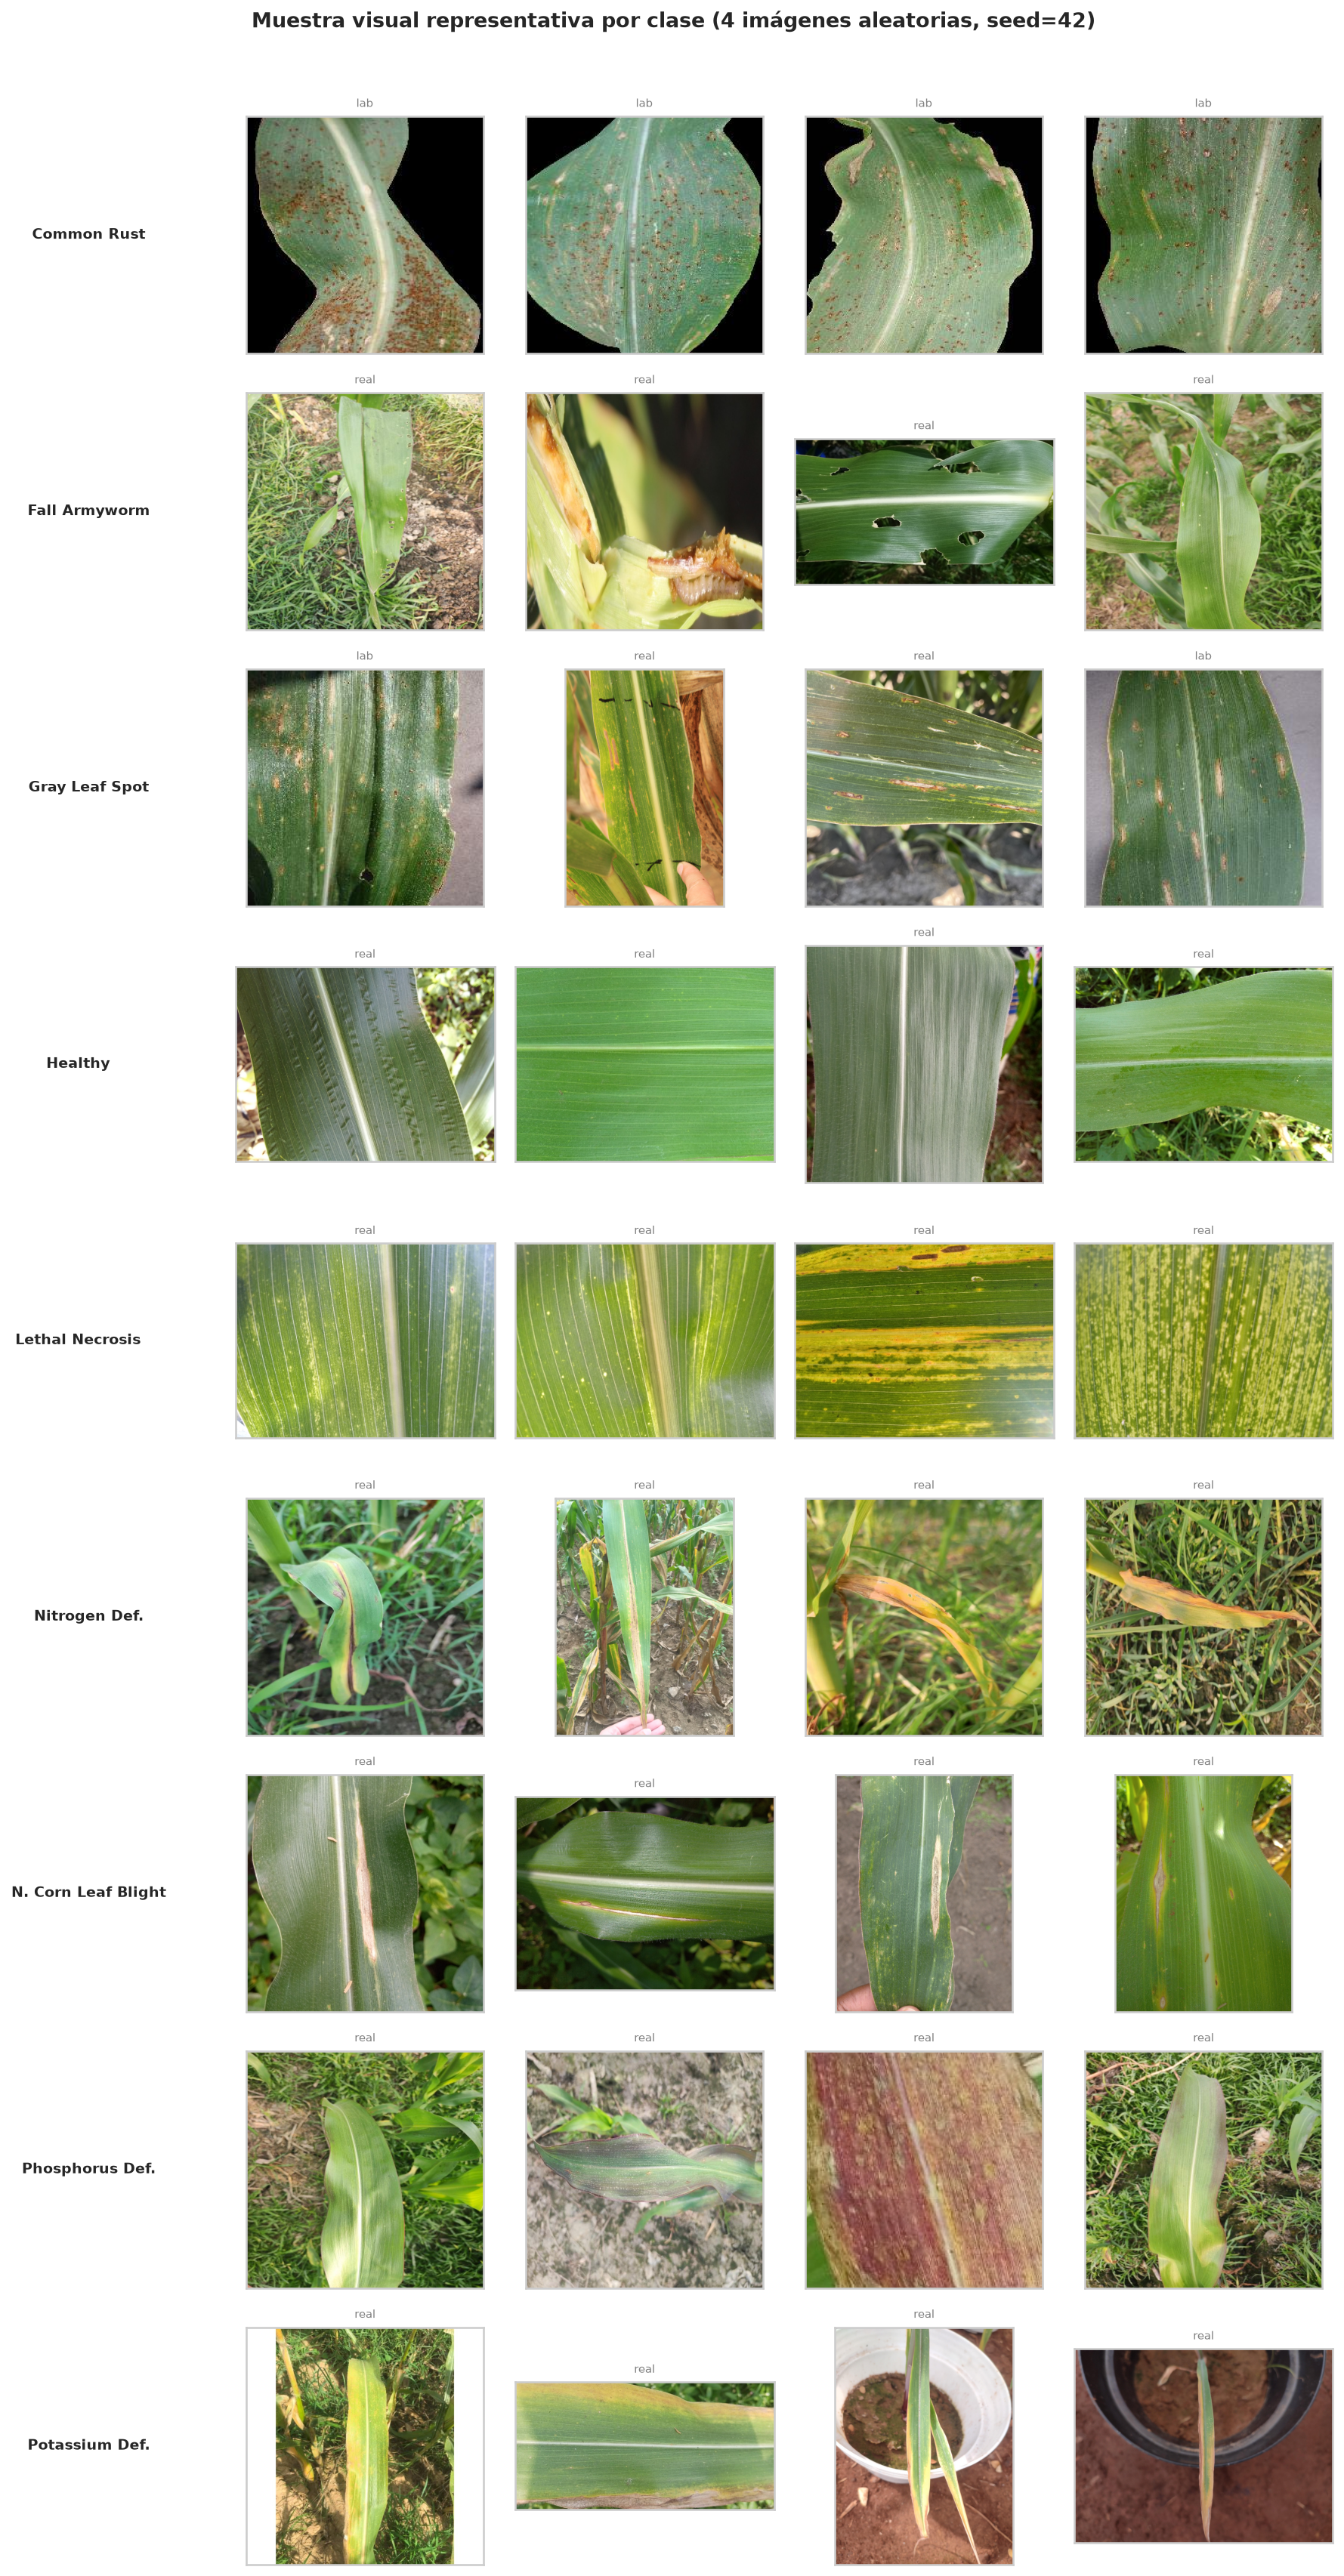
\includegraphics[height=0.74\textheight,keepaspectratio]{images/eda/eda_00_muestra_visual.png}
\caption{Diversidad morfol\'ogica, fondos r\'usticos y heterogeneidad geom\'etrica en las afecciones foliares del ma\'iz.}
\label{fig:eda_samples}
\end{figure}

\subsection{Planteamiento del problema}

A partir de la situaci\'on descrita, se constata que los mecanismos tradicionales de extensi\'on agron\'omica resultan insuficientes para brindar cobertura a los peque\~nos productores de ma\'iz en El Salvador, mientras que las herramientas digitales contempor\'aneas han sido concebidas bajo premisas incompatibles con la realidad rural. En la pr\'actica, las soluciones comerciales de visi\'on artificial presentan tres limitaciones cr\'iticas:

\begin{enumerate}
\item \textbf{Dependencia de conectividad de red:} La mayor parte de las aplicaciones disponibles requieren comunicaci\'on permanente con servidores en la nube para procesar las capturas. En el agro salvadore\~no, donde extensas zonas rurales presentan cobertura celular inestable o nula y los agricultores no disponen de planes continuos de transmisi\'on de datos, esta dependencia anula la utilidad pr\'actica de las herramientas en el propio surco.
\item \textbf{Incompatibilidad con terminales b\'asicos:} Los modelos de aprendizaje profundo convencionales demandan una capacidad de c\'omputo y memoria que excede con creces los recursos de los tel\'efonos inteligentes accesibles para las familias campesinas (dispositivos de gama de entrada con 2 a 4~GB de RAM), provocando bloqueos, latencias intolerables y un r\'apido consumo de bater\'ia.
\item \textbf{Vulnerabilidad ante la variabilidad del entorno real:} Al haber sido entrenados mayoritariamente sobre im\'agenes de laboratorio con fondos neutros e iluminaci\'on homog\'enea, los algoritmos colapsan al exponerse a la milpa, donde la presencia de suelos r\'usticos, sombras irregulares, malezas y contraluz induce clasificaciones err\'oneas emitidas con un alto grado de sobreconfianza.
\end{enumerate}

Frente a este escenario, surge la necesidad de replantear el diagn\'ostico automatizado desde las restricciones materiales del entorno agr\'icola. Una herramienta orientada a cerrar esta brecha debe operar directamente en manos del productor, fundament\'andose en cuatro requerimientos operacionales esenciales:

\begin{itemize}
\item \textbf{Autonom\'ia operativa local:} La capacidad diagn\'ostica debe ejecutarse de forma integral en el propio dispositivo, asegurando disponibilidad inmediata en la parcela sin supeditar su funcionamiento a redes de telecomunicaciones.
\item \textbf{Austeridad y eficiencia computacional:} El procesamiento debe ajustarse estrictamente a las capacidades t\'ecnicas de los tel\'efonos b\'asicos predominantes en las zonas rurales, garantizando tiempos de respuesta cortos y un consumo m\'inimo de energ\'ia.
\item \textbf{Resiliencia y bioseguridad ante la captura:} El sistema debe ser capaz de discriminar la sintomatolog\'ia foliar frente al ruido visual del campo y, de manera primordial, reconocer situaciones de incertidumbre o tomas no v\'alidas para abstenerse de emitir diagn\'osticos infundados que perjudiquen la econom\'ia familiar.
\item \textbf{Traducci\'on agron\'omica orientada a la acci\'on:} El diagn\'ostico visual debe complementarse con una evaluaci\'on comprensible del nivel de da\~no y con alternativas concretas de manejo integrado basadas en bioinsumos accesibles, facilitando una intervenci\'on oportuna y viable para el productor.
\end{itemize}

Con base en estas consideraciones, se formula la problem\'atica central de la investigaci\'on:
\begin{quote}
\centering
\itshape
\textquestiondown En qu\'e medida es factible concebir, desarrollar y evaluar una aplicaci\'on m\'ovil de diagn\'ostico fitosanitario que opere de manera aut\'onoma en tel\'efonos inteligentes de gama baja o media, capaz de discernir patolog\'ias foliares en condiciones reales de campo, gestionar la incertidumbre de la captura y orientar oportunamente al agricultor salvadore\~no en el manejo integrado de su cultivo?
\end{quote}

\subsubsection{Modelo conceptual de caja negra del sistema}

Con el prop\'osito de delimitar anal\'iticamente este problema sin prejuzgar la arquitectura interna que deber\'a investigarse y validarse experimentalmente en los cap\'itulos posteriores, el sistema se conceptualiza mediante el modelo de caja negra (Figura~\ref{fig:caja_negra}). En la ingenier\'ia de sistemas, este enfoque formaliza la relaci\'on entre los est\'imulos y restricciones del entorno problem\'atico (entradas) y los resultados requeridos para mitigar la problem\'atica (salidas), definiendo el n\'ucleo del sistema como el proceso de transformaci\'on tecnol\'ogica que constituye el objeto de estudio de esta investigaci\'on:

\begin{figure}[H]
\centering
\resizebox{0.98\textwidth}{!}{%
\begin{tikzpicture}[
    node distance=1.0cm and 0.9cm,
    header/.style={
        rectangle,
        rounded corners=3pt,
        minimum width=5.2cm,
        minimum height=0.75cm,
        text centered,
        font=\bfseries\small,
        text=white
    },
    card/.style={
        rectangle,
        rounded corners=5pt,
        minimum width=5.3cm,
        text width=4.9cm,
        inner sep=8pt,
        font=\scriptsize,
        draw=gray!35,
        line width=1pt,
        align=left
    },
    arrow/.style={
        -{Latex[length=3.5mm,width=2.5mm]},
        line width=1.8pt,
        draw=gray!70
    }
]

% --- COLUMNA 1: ENTRADA ---
\node[header, fill=blue!75!black] (head_in) {Entradas};
\node[card, fill=blue!3, below=0.15cm of head_in] (box_in) {
  \textbf{Condiciones del Entorno Rural:}
  \begin{itemize}\setlength{\itemsep}{2pt}\setlength{\leftskip}{-10pt}
    \item Fotograf\'ias foliares capturadas por el agricultor en parcelas reales.
    \item Iluminaci\'on solar directa no uniforme, sombras duras y fondos r\'usticos.
    \item Sintomatolog\'ia foliar diversa y estados fenol\'ogicos heterog\'eneos.
  \end{itemize}
  \vspace{0.12cm}
  \textbf{Restricciones Operativas del Problema:}
  \begin{itemize}\setlength{\itemsep}{2pt}\setlength{\leftskip}{-10pt}
    \item Ausencia total de conectividad m\'ovil o internet en el surco.
    \item Tel\'efonos inteligentes b\'asicos con recursos acotados de memoria y procesador.
  \end{itemize}
};

% --- COLUMNA 2: CAJA NEGRA (PROCESO) ---
\node[header, fill=gray!80!black, right=1.4cm of head_in] (head_proc) {Procesos};
\node[card, fill=gray!4, below=0.15cm of head_proc] (box_proc) {
  \textbf{Transformaci\'on Requerida:}
  \begin{itemize}\setlength{\itemsep}{2pt}\setlength{\leftskip}{-10pt}
    \item Procesamiento y an\'alisis visual local en el dispositivo m\'ovil.
    \item Discriminaci\'on de afecciones foliares frente al ruido del entorno.
    \item Evaluaci\'on de confiabilidad y validez de la captura realizada.
    \item Vinculaci\'on de la evidencia \'optica con directrices agron\'omicas.
  \end{itemize}
  \vspace{0.12cm}
  \textbf{Desaf\'io de Ingenier\'ia e Investigaci\'on:}
  \begin{itemize}\setlength{\itemsep}{2pt}\setlength{\leftskip}{-10pt}
    \item \textquestiondown C\'omo lograr sensibilidad diagn\'ostica y resiliencia ante entornos r\'usticos dentro de los l\'imites estrictos de un m\'ovil modesto?
  \end{itemize}
};

% --- COLUMNA 3: SALIDA ESPERADA ---
\node[header, fill=teal!70!black, right=1.4cm of head_proc] (head_out) {Salidas esperadas};
\node[card, fill=teal!3, below=0.15cm of head_out] (box_out) {
  \textbf{Diagn\'ostico y Bioseguridad:}
  \begin{itemize}\setlength{\itemsep}{2pt}\setlength{\leftskip}{-10pt}
    \item Detecci\'on temprana y diferenciada de la afecci\'on foliar evaluada.
    \item Alta sensibilidad en patolog\'ias cr\'iticas para evitar p\'erdidas totales.
    \item Distinci\'on confiable entre plagas, enfermedades y deficiencias nutricionales.
  \end{itemize}
  \vspace{0.12cm}
  \textbf{Decisi\'on Fitosanitaria en Parcela:}
  \begin{itemize}\setlength{\itemsep}{2pt}\setlength{\leftskip}{-10pt}
    \item Alerta preventiva y abstenci\'on ante im\'agenes dudosas («No reconocida»).
    \item Orientaci\'on de severidad y bioinsumos en lenguaje claro y accesible.
    \item Prevenci\'on del gasto infructuoso en agroqu\'imicos inapropiados.
  \end{itemize}
};

% --- FLECHAS DE CONEXIÓN ---
\draw[arrow] (box_in.east) -- (box_proc.west);
\draw[arrow] (box_proc.east) -- (box_out.west);

\end{tikzpicture}%
}
\caption{Modelo conceptual de caja negra para el diagn\'ostico fitosanitario m\'ovil.}
\label{fig:caja_negra}
\end{figure}

Como sintetiza la Figura~\ref{fig:caja_negra}, el modelo de caja negra formaliza la l\'ogica de la investigaci\'on: establece c\'omo las restricciones de campo y los desaf\'ios visuales del cultivo ingresan a un proceso de transformaci\'on m\'ovil concebido para generar diagn\'osticos confiables y decisiones fitosanitarias oportunas para el campesino. A partir de esta delimitaci\'on del problema, se formulan a continuaci\'on los objetivos de la investigaci\'on.

\section{Objetivos}

\subsection{Objetivo General}

Desarrollar, evaluar e implementar un sistema de visi\'on artificial embebido (\textit{Edge AI}) para el diagn\'ostico fitosanitario a partir de im\'agenes de la hoja de ma\'iz en El Salvador, desplegado mediante una aplicaci\'on m\'ovil nativa de operaci\'on completamente desconectada (\textit{offline}), capaz de clasificar afecciones foliares con alta sensibilidad y baja latencia en tel\'efonos inteligentes de gama baja o media.

\subsection{Objetivos Espec\'ificos}

\begin{enumerate}
\item Consolidar, depurar y auditar criptogr\'aficamente un conjunto multimodal de m\'as de 33~000 im\'agenes de la hoja de ma\'iz distribuidas en 9 condiciones agron\'omicas, estableciendo contratos de datos verificables para descartar duplicados y prevenir filtraciones entre particiones.
\item Optimizar arquitecturas convolucionales ligeras preentrenadas mediante b\'usqueda bayesiana de hiperpar\'ametros (Optuna) y algoritmos de poda temprana, maximizando el Macro $F_1$-Score con un uso eficiente del c\'omputo en GPU.
\item Dise\~nar una estrategia de ensamble por votaci\'on suave (\textit{Soft Voting}) que combine modelos con diferentes sesgos inductivos, con el fin de elevar la sensibilidad diagn\'ostica en patolog\'ias cr\'iticas de la hoja de ma\'iz y mitigar el desbalance de clases.
\item Evaluar el desempe\~no del sistema bajo protocolos de validaci\'on cruzada agrupada por procedencia (\textit{SourceGroupedKFold}), cuantificando la disparidad de impacto entre laboratorio y campo real, as\'i como la atribuci\'on espacial mediante t\'ecnicas de explicabilidad y ablaci\'on de fondo.
\item Cuantizar la arquitectura neuronal a enteros de 8 bits (Int8) e integrarla en una aplicaci\'on m\'ovil nativa provista de marco gu\'ia de encuadre y detector de tomas an\'omalas, validando su precisi\'on y fluidez en tel\'efonos inteligentes f\'isicos de gama baja o media.
\item Formular una propuesta estrat\'egica de integraci\'on institucional y pol\'iticas p\'ublicas orientada al Ministerio de Agricultura y Ganader\'ia (MAG) y al CENTA, que facilite la transferencia tecnol\'ogica y el acompa\~namiento t\'ecnico a los peque\~nos productores de ma\'iz.
\end{enumerate}

\section{Alcance y L\'imites del Proyecto}

\subsection{Alcance del Proyecto}

El alcance del presente proyecto comprende la investigaci\'on, dise\~no, desarrollo e implementaci\'on de una soluci\'on integral de diagn\'ostico fitosanitario orientada a los peque\~nos productores de ma\'iz en El Salvador. La soluci\'on se materializa en dos componentes tecnol\'ogicos articulados: la aplicaci\'on m\'ovil nativa para el usuario final y el motor anal\'itico de visi\'on artificial embebida.

\subsubsection{Alcance de la Aplicaci\'on M\'ovil (DoctorMaiz)}
La aplicaci\'on m\'ovil constituye el punto de interacci\'on directa en manos del agricultor y abarca las siguientes capacidades funcionales:
\begin{itemize}
\item \textbf{Inferencia local aut\'onoma (\textit{Offline}):} Ejecuci\'on integral del motor neuronal en el procesador del tel\'efono mediante modelos cuantizados, asegurando diagn\'osticos instant\'aneos en el surco sin requerir conexi\'on a internet ni datos m\'oviles.
\item \textbf{Captura asistida con marco gu\'ia foliar:} Interfaz de c\'amara con ret\'icula visual ergon\'omica que orienta al agricultor a encuadrar la l\'amina de la hoja, reduciendo la captura de fondos distractores (suelo, sombras o maleza) antes de procesar la imagen.
\item \textbf{Detecci\'on preventiva de capturas an\'omalas (Seguridad OOD):} M\'odulo de rechazo ante muestras fuera de dominio capaz de evaluar si la captura no corresponde a una hoja de ma\'iz o presenta incertidumbre excesiva, notificando un estado de «No reconocida» para evitar diagn\'osticos enga\~nosos.
\item \textbf{Diagn\'ostico y valoraci\'on de severidad:} Presentaci\'on de resultados en lenguaje claro y accesible, categorizando la afecci\'on con una escala visual de severidad en tres niveles (leve, moderada y severa) para apoyar la toma de decisiones.
\item \textbf{Cat\'alogo de manejo integrado y bioinsumos:} Gu\'ia fitosanitaria pr\'actica vinculada al diagn\'ostico que ofrece alternativas de bioinsumos y manejo cultural de bajo costo, previniendo gastos perjudiciales en agroqu\'imicos inapropiados.
\item \textbf{Historial y georreferenciaci\'on de muestreos:} Registro local persistente de cada evaluaci\'on (fecha, diagn\'ostico, severidad y ubicaci\'on GPS) para que el agricultor monitoree la evoluci\'on de sus parcelas a lo largo del ciclo agr\'icola.
\item \textbf{Contribuci\'on comunitaria y sincronizaci\'on voluntaria:} M\'odulo opcional que permite almacenar im\'agenes validadas localmente para compartirlas cuando se cuente con conectividad, contribuyendo al monitoreo fitosanitario colectivo.
\end{itemize}

\subsubsection{Alcance del Componente de Inteligencia Artificial Embebida}
El n\'ucleo de aprendizaje profundo embebido abarca:
\begin{itemize}
\item \textbf{Cobertura taxon\'omica de 9 clases en hoja de ma\'iz:} Clasificaci\'on supervisada de signos y s\'intomas foliares, cubriendo enfermedades causadas por hongos (tiz\'on foliar, mancha gris y roya com\'un), virosis cr\'itica (necrosis letal del ma\'iz), plagas directas (gusano cogollero), deficiencias nutricionales de suelo (nitr\'ogeno, f\'osforo y potasio) y l\'amina foliar sana.
\item \textbf{Optimizaci\'on bayesiana, ensamble y cuantizaci\'on Int8:} B\'usqueda automatizada de hiperpar\'ametros (Optuna con poda temprana), combinaci\'on estrat\'egica por votaci\'on suave (\textit{Soft Voting}) y cuantizaci\'on a 8 bits exportada en formato TensorFlow Lite mediante litert-torch, optimizada para inferencia ultrarr\'apida ($\le 100$~ms) en procesadores m\'oviles.
\item \textbf{Auditor\'ia de sesgos y generalizaci\'on:} Protocolo de evaluaci\'on cruzada agrupada por procedencia (\textit{SourceGroupedKFold}) y pruebas de ablaci\'on espacial de fondo para auditar y neutralizar el fen\'omeno de atajos visuales (\textit{Clever Hans effect}).
\end{itemize}

\subsection{L\'imites y Fronteras del Proyecto}

Con el fin de delimitar con precisi\'on la cobertura de la investigaci\'on, se definen los siguientes l\'imites operacionales:
\begin{itemize}
\item \textbf{L\'imite biol\'ogico y sintom\'atico:} El sistema se restringe exclusivamente al an\'alisis de afecciones visibles en la l\'amina foliar del ma\'iz. Quedan fuera del alcance patolog\'ias radiculares, afecciones del tallo interno sin expresi\'on foliar y el monitoreo de plagas subterr\'aneas.
\item \textbf{L\'imite de plataforma y compatibilidad de hardware:} La soluci\'on m\'ovil se enfoca en dispositivos con sistema operativo Android 7.0 o superior con arquitectura de procesador ARM (v7 o v8), c\'amara trasera con enfoque autom\'atico y al menos 2~GB de memoria RAM. No se contempla desarrollo nativo para iOS ni para tel\'efonos sin capacidades inteligentes.
\item \textbf{L\'imite de infraestructura y red:} La aplicaci\'on est\'a dise\~nada para operar desconectada; no existe dependencia de servicios en la nube para emitir el diagn\'ostico, ni se incluye sincronizaci\'on transaccional en tiempo real entre m\'ultiples terminales.
\item \textbf{L\'imite legal y de diagn\'ostico fitopatol\'ogico:} La herramienta constituye un asistente t\'ecnico de orientaci\'on y apoyo agron\'omico para el productor. En ning\'un caso reemplaza los ensayos fitopatol\'ogicos de laboratorio (cultivos, aislamiento microbiano o pruebas PCR), ni sustituye los dict\'amenes oficiales de cuarentena o certificaci\'on fitosanitaria del Ministerio de Agricultura y Ganader\'ia.
\end{itemize}

\section{Hip\'otesis}

\subsection{Hip\'otesis General}
El dise\~no propone un sistema de visi\'on artificial embebido en una aplicaci\'on m\'ovil nativa, con captura asistida y operaci\'on completamente desconectada, capaz de clasificar nueve condiciones agron\'omicas de la hoja de ma\'iz en tel\'efonos inteligentes de gama baja o media del sector rural salvadore\~no. Se considera alcanzado el objetivo general si se cumplen los criterios de la Tabla~\ref{tab:criterios_exito}.

\subsection{Criterios de \'Exito Espec\'ificos}
Los criterios siguientes son las condiciones que el sistema debe cumplir para considerar alcanzado cada objetivo. Se verifican en el cap\'itulo de resultados y se agrupan en cuatro temas.

\begin{table}[H]
\caption{Criterios de \'exito del proyecto, agrupados por tema}
\label{tab:criterios_exito}
\centering
\small
\begin{singlespace}
\begin{tabularx}{\textwidth}{>{\raggedright\arraybackslash}p{3.4cm}>{\raggedright\arraybackslash}X>{\raggedright\arraybackslash}p{3.2cm}}
\toprule
\textbf{Tema} & \textbf{Criterio y umbral} & \textbf{M\'etrica} \\
\midrule
Ahorro de entrenamiento & Reducir en al menos 40\% las horas de GPU frente a una b\'usqueda sin poda temprana. & Horas de GPU por corrida \\
Rendimiento del modelo & Alcanzar Macro $F_1 \ge 0.85$ en la partici\'on de prueba retenida, con recall de la necrosis letal (MLN) $\ge 95\%$. & Macro $F_1$, recall por clase \\
Capacidades del diagn\'ostico & Mantener un \textit{Disparate Impact Ratio} $\ge 0.80$ entre laboratorio y campo real, y rechazar fuera de dominio las im\'agenes que no son hojas de ma\'iz. & DIR, umbral OOD \\
Soluci\'on integral & Modelo Int8 menor a 5~MB, inferencia en menos de 100~ms en un tel\'efono de gama media y funcionamiento sin conexi\'on. & Tama\~no, latencia \\
\bottomrule
\end{tabularx}
\end{singlespace}
\end{table}

\section{Justificaci\'on}

\subsection{Justificaci\'on T\'ecnica y Metodol\'ogica}
La presente investigaci\'on se justifica t\'ecnicamente al trasladar el procesamiento de aprendizaje profundo desde arquitecturas dependientes de servidores en la nube hacia el borde del dispositivo m\'ovil (\textit{Edge AI}). En la literatura especializada de visi\'on por computadora aplicada a la agricultura, predomina el entrenamiento de modelos convolucionales de alta complejidad evaluados sobre particiones aleatorias convencionales, las cuales frecuentemente sufren de fuga de informaci\'on e introducen atajos visuales ligados a fondos controlados \cite{ahmad2023a}. El presente proyecto aborda esta limitaci\'on mediante una metodolog\'ia rigurosa basada en auditor\'ia de duplicados a nivel de p\'ixel, esquemas de validaci\'on cruzada agrupada por procedencia y t\'ecnicas de cuantizaci\'on sim\'etrica a enteros de 8 bits (\textit{Int8}) que reducen dr\'asticamente la demanda computacional sin comprometer la sensibilidad diagn\'ostica \cite{howard2017,tan2019}. Asimismo, integra salvaguardas operacionales como el filtrado de muestras fuera de dominio (\textit{OOD}) \cite{lee2018} y mecanismos de explicabilidad visual mediante mapas de activaci\'on \cite{selvaraju2017}, con el fin de que las predicciones se apoyen en caracter\'isticas de la l\'amina foliar; la verificaci\'on de este objetivo se presenta en el cap\'itulo de resultados.

\subsection{Justificaci\'on Econ\'omica}
Para las peque\~nas familias productoras de ma\'iz en El Salvador, el margen de rentabilidad agr\'icola por ciclo es sumamente reducido y altamente vulnerable a sobrecostos imprevistos \cite{mag2023}. Un diagn\'ostico fitosanitario err\'oneo conduce a la compra e intoxicaci\'on del cultivo con agroqu\'imicos comerciales inadecuados, mermando el escaso capital de trabajo disponible. Proveer una aplicaci\'on m\'ovil de uso aut\'onomo, gratuito y local en el propio tel\'efono inteligente del agricultor permite orientar de manera precisa la intervenci\'on fitosanitaria, evitando gastos innecesarios en plaguicidas ante s\'intomas provocados por deficiencias nutricionales y facilitando una acci\'on temprana contra plagas destructivas como el gusano cogollero (\textit{Spodoptera frugiperda}) antes de que comprometan el rendimiento econ\'omico de la milpa \cite{centa2022}.

\subsection{Justificaci\'on Social y Ambiental}
Desde la perspectiva social, la implementaci\'on de \textit{DoctorMaiz} contribuye a reducir la brecha tecnol\'ogica en comunidades rurales con acceso limitado o nulo a servicios presenciales de extensi\'on agron\'omica \cite{centa2022}. Al transformar un tel\'efono celular com\'un de gama baja o media en un asistente de orientaci\'on fitopatol\'ogica disponible en el surco, se empodera al productor con informaci\'on t\'ecnica comprensible y oportuna. En la dimensi\'on ambiental, un diagn\'ostico certero fomenta el manejo integrado de plagas, desincentivando la aplicaci\'on indiscriminada de pesticidas sint\'eticos y coadyuvando a la protecci\'on de los recursos h\'idricos y la salud de las comunidades rurales.

\subsection{Justificaci\'on Acad\'emica e Institucional}
En el \'ambito acad\'emico e institucional, este proyecto representa una contribuci\'on significativa para la Escuela de Ingenier\'ia de Sistemas Inform\'aticos de la Universidad de El Salvador (UES), al articular la investigaci\'on aplicada en inteligencia artificial embebida con la soluci\'on de problemas prioritarios del desarrollo agropecuario nacional. La investigaci\'on sienta un precedente metodol\'ogico formal para el desarrollo, evaluaci\'on imparcial y despliegue de sistemas de visi\'on artificial adaptados a contextos de recursos computacionales y conectividad restringidos en Centroam\'erica.

\section{Cronograma de Actividades}

La planificaci\'on y ejecuci\'on del proyecto se estructur\'o bajo las fases de la metodolog\'ia \textit{CRISP-DM} (\textit{Cross-Industry Standard Process for Data Mining}), adaptada a los requerimientos de desarrollo de aprendizaje profundo embebido (\textit{Edge AI}) e ingenier\'ia de software m\'ovil. El cronograma abarc\'o un periodo de 28 semanas calendario, iniciando formalmente el 14 de abril de 2026 y culminando con el hito de presentaci\'on y defensa final el 29 de octubre de 2026.

La Figura~\ref{fig:gantt_cronograma} ilustra el diagrama temporal de Gantt y la concurrencia operativa de las fases a lo largo de las 28 semanas del ciclo, mientras que la Tabla~\ref{tab:cronograma} detalla la distribuci\'on de actividades, duraci\'on, horas estimadas y entregables t\'ecnicos por cada etapa.

\begin{figure}[H]
\centering
\caption{Diagrama de Gantt de ejecuci\'on temporal del proyecto (Metodolog\'ia CRISP-DM)}
\label{fig:gantt_cronograma}
\resizebox{\textwidth}{!}{%
\begin{ganttchart}[
    vgrid={draw=black!15, line width=.4pt},
    hgrid={draw=black!10, line width=.4pt},
    canvas/.append style={draw=black!30, line width=.75pt},
    title/.style={draw=black!30, fill=black!5},
    title label font=\bfseries\small,
    bar/.append style={line width=.5pt, rounded corners=2pt},
    bar height=.6,
    bar label font=\small,
    milestone/.append style={line width=.5pt},
    milestone height=.65,
    milestone label font=\bfseries\small,
    x unit=0.52cm,
    y unit chart=0.75cm,
    y unit title=0.6cm
]{1}{28}
\gantttitle{Abr}{3} \gantttitle{May}{4} \gantttitle{Jun}{4} \gantttitle{Jul}{5} \gantttitle{Ago}{4} \gantttitle{Sep}{4} \gantttitle{Oct}{4} \\
\gantttitle{S1--3}{3} \gantttitle{S4--7}{4} \gantttitle{S8--11}{4} \gantttitle{S12--16}{5} \gantttitle{S17--20}{4} \gantttitle{S21--24}{4} \gantttitle{S25--28}{4} \\
\ganttbar[bar/.append style={fill=blue!65!black, draw=blue!90!black}]{Fase 1: Negocio y Datos}{1}{4} \\
\ganttbar[bar/.append style={fill=cyan!65!black, draw=cyan!90!black}]{Fase 2: Preparaci\'on de Datos}{5}{8} \\
\ganttbar[bar/.append style={fill=teal!70!black, draw=teal!90!black}]{Fase 3: Modelado y Optuna}{9}{14} \\
\ganttbar[bar/.append style={fill=orange!75!black, draw=orange!90!black}]{Fase 4: Evaluaci\'on y Sesgos}{15}{18} \\
\ganttbar[bar/.append style={fill=green!60!black, draw=green!80!black}]{Fase 5: Edge AI y App M\'ovil}{19}{24} \\
\ganttbar[bar/.append style={fill=purple!65!black, draw=purple!90!black}]{Fase 6: Pruebas y Memoria}{25}{28} \\
\ganttmilestone[milestone/.append style={fill=red!80!black, draw=red!90!black}]{Hito: Defensa Final (29/10)}{28}
\end{ganttchart}%
}
\end{figure}

\begin{table}[H]
\caption{Cronograma consolidado de actividades y fases del proyecto (CRISP-DM)}
\label{tab:cronograma}
\centering
\small
\begin{singlespace}
\begin{tabularx}{\textwidth}{p{4.3cm}ccccX}
\toprule
\textbf{Fase / Actividad Operativa} & \textbf{Inicio} & \textbf{Fin} & \textbf{Semanas} & \textbf{Horas} & \textbf{Entregable Principal} \\
\midrule
\textbf{Fase 1: Comprensi\'on del Negocio y Datos} & 14/04/26 & 12/05/26 & 4 & 40 h & Requisitos fitosanitarios y corpus consolidado ($>$33K im\'agenes). \\
\textbf{Fase 2: Preparaci\'on de Datos} & 12/05/26 & 09/06/26 & 4 & 40 h & Auditor\'ia criptogr\'afica de duplicados, balanceo y data augmentation. \\
\textbf{Fase 3: Modelado Algor\'itmico} & 09/06/26 & 21/07/26 & 6 & 60 h & Transfer learning en arquitecturas ligeras y optimizaci\'on con Optuna. \\
\textbf{Fase 4: Evaluaci\'on y Auditor\'ia de Sesgos} & 21/07/26 & 18/08/26 & 4 & 40 h & Ensamble Soft Voting, evaluaci\'on ciega de campo y an\'alisis XAI (Grad-CAM). \\
\textbf{Fase 5: Optimizaci\'on Edge y App M\'ovil} & 18/08/26 & 29/09/26 & 6 & 60 h & Modelo Int8 (3.56~MB), detector OOD y app DoctorMaiz (React Native/Expo). \\
\textbf{Fase 6: Pruebas Finales y Memoria} & 29/09/26 & 29/10/26 & 4 & 40 h & Evaluaci\'on f\'isica en Motorola edge 40 neo, memoria t\'ecnica y defensa final. \\
\midrule
\textbf{Hito Final: Defensa de Proyecto} & \multicolumn{2}{c}{\textbf{29 de octubre de 2026}} & \textbf{28 sem} & \textbf{280 h} & \textbf{Sistema DoctorMaiz liberado} \\
\bottomrule
\end{tabularx}
\end{singlespace}
\end{table}

\section{Presupuesto Global Estimado}

El presupuesto del desarrollo y evaluaci\'on de la soluci\'on anal\'itica y embebida abarc\'o dos categor\'ias esenciales: recurso humano especializado e infraestructura de c\'omputo acelerado en la nube (Tablas~\ref{tab:presupuesto_rh} a~\ref{tab:presupuesto_resumen}). Las horas de GPU se tomaron de los registros de ejecuci\'on del repositorio; el resto de rubros son proyecciones.

\begin{table}[H]
\caption{Presupuesto proyectado: C\'alculo del salario base por rol (280 horas)}
\label{tab:presupuesto_rh}
\centering
\small
\begin{singlespace}
\begin{tabularx}{\textwidth}{>{\raggedright\arraybackslash}X>{\centering\arraybackslash}p{2.6cm}>{\centering\arraybackslash}p{2.6cm}>{\centering\arraybackslash}p{2.6cm}>{\centering\arraybackslash}p{2.6cm}}
\toprule
\textbf{Rol Profesional} & \textbf{Salario mensual de referencia} & \textbf{Meses equivalentes (280 h)} & \textbf{Salario base (USD)} \\
\midrule
Ingeniero de Datos / MLOps & \$1,500.00 & 1.6154 & \$2,423.08 \\
Investigador de Deep Learning & \$1,350.00 & 1.6154 & \$2,180.77 \\
Desarrollador M\'ovil Edge AI & \$1,250.00 & 1.6154 & \$2,019.23 \\
\midrule
\textbf{Total salario base} & \textbf{\$4,100.00} & — & \textbf{\$6,623.08} \\
\bottomrule
\end{tabularx}
\end{singlespace}
\end{table}

\begin{table}[H]
\caption{Presupuesto proyectado: Cargas y prestaciones patronales sobre el salario base}
\label{tab:presupuesto_cargas}
\centering
\small
\begin{singlespace}
\begin{tabularx}{\textwidth}{>{\raggedright\arraybackslash}X>{\centering\arraybackslash}p{1.75cm}>{\centering\arraybackslash}p{1.75cm}>{\centering\arraybackslash}p{1.75cm}>{\centering\arraybackslash}p{2.0cm}>{\centering\arraybackslash}p{1.75cm}>{\centering\arraybackslash}p{2.0cm}}
\toprule
\textbf{Rol Profesional} & \textbf{ISSS 7.5\%} & \textbf{AFP 7.75\%} & \textbf{INSAFORP 1\%} & \textbf{Aguinaldo y vacaciones} & \textbf{Total cargas} & \textbf{Costo total} \\
\midrule
Ingeniero de Datos / MLOps & \$121.15 & \$187.79 & \$24.23 & \$201.92 & \$535.09 & \$2,958.17 \\
Investigador de Deep Learning & \$121.15 & \$169.01 & \$21.81 & \$181.73 & \$493.70 & \$2,674.47 \\
Desarrollador M\'ovil Edge AI & \$121.15 & \$156.49 & \$20.19 & \$168.27 & \$466.10 & \$2,485.33 \\
\midrule
\textbf{Total Recurso Humano} & \textbf{\$363.45} & \textbf{\$513.29} & \textbf{\$66.23} & \textbf{\$551.92} & \textbf{\$1,494.89} & \textbf{\$8,117.97} \\
\bottomrule
\end{tabularx}
\end{singlespace}
\end{table}

Los salarios mensuales corresponden al punto medio de la escala de referencia del sector p\'ublico salvadore\~no para Gobierno Central y Ministerios, aplicada a perfiles equivalentes: Ingeniero de Datos / MLOps (rango de \$1,200 a \$1,800, equivalente a Especialista de Base de Datos o Analista de Sistemas), Investigador de Deep Learning (rango de \$1,100 a \$1,600, equivalente a Especialista en An\'alisis de Datos) y Desarrollador M\'ovil (rango de \$1,000 a \$1,500, equivalente a Analista Programador). La Tabla~\ref{tab:presupuesto_rh} calcula el salario base por rol y la Tabla~\ref{tab:presupuesto_cargas} desglosa las cargas patronales y el costo total. El costo se estima solo por las horas efectivas de trabajo. Cada integrante trabaja de lunes a viernes, menos de 2 horas diarias; para la estimaci\'on se usan 2 horas diarias como cota superior, es decir 10 horas semanales, lo que suma 280 horas en las 28 semanas del cronograma (Tabla~\ref{tab:cronograma}). Equivale a 1.62 meses de una jornada de 40 horas, por lo que el salario mensual de referencia se prorrateó por esa proporci\'on. Las cargas consideran: cuota patronal al ISSS de 7.5\% sobre un salario base m\'aximo de \$1,000.00 mensual; cuota patronal a la AFP de 7.75\%; contribuci\'on al INSAFORP de 1\%; y aguinaldo y vacaciones de ley prorrateados.

\begin{table}[H]
\caption{Presupuesto: Infraestructura Cloud y Licencias}
\label{tab:presupuesto_hw}
\centering
\small
\begin{singlespace}
\begin{tabularx}{\textwidth}{>{\raggedright\arraybackslash}p{3.8cm}>{\raggedright\arraybackslash}X>{\raggedright\arraybackslash}p{4.0cm}>{\raggedleft\arraybackslash}p{2.0cm}}
\toprule
\textbf{Rubro} & \textbf{Detalle T\'ecnico} & \textbf{M\'etrica / Cantidad} & \textbf{Subtotal} \\
\midrule
Instancias GPU Modal & NVIDIA A10G (24 GB VRAM) & 15.85 horas medidas $\times$ \$1.10/h & \$17.44 \\
Almacenamiento Cloud & Cloud Volumes y respaldos de pesos & 100 GB $\times$ 6 meses & \$30.00 \\
Licenciamiento software & PyTorch, Expo, React Native, Optuna & Licencias Open Source / MIT & \$0.00 \\
\midrule
\textbf{Total Infraestructura Cloud y Licencias} & — & — & \textbf{\$47.44} \\
\bottomrule
\end{tabularx}
\end{singlespace}
\end{table}

\begin{table}[H]
\caption{Resumen presupuestario global de la investigaci\'on}
\label{tab:presupuesto_resumen}
\centering
\small
\begin{singlespace}
\begin{tabular}{lcc}
\toprule
\textbf{Rubro de Inversi\'on} & \textbf{Monto Total (USD)} & \textbf{Porcentaje (\%)} \\
\midrule
Recursos Humanos de Investigaci\'on & \$8,117.97 & 99.42\% \\
Servicios de c\'omputo en la nube (GPU/Storage) & \$47.44 & 0.58\% \\
\midrule
\textbf{Total General} & \textbf{\$8,165.41} & \textbf{100.00\%} \\
\bottomrule
\end{tabular}
\end{singlespace}
\end{table}

La ejecuci\'on financiera demuestra que, gracias al aprovechamiento de tecnolog\'ias de c\'odigo abierto y la utilizaci\'on estrat\'egica de cl\'usteres serverless con parada autom\'atica, el costo directo de infraestructura computacional se mantuvo en valores extraordinariamente accesibles (\$47.44 USD, de los cuales \$17.44 corresponden a las 15.85 horas de GPU medidas y \$30.00 al almacenamiento), ratificando la viabilidad econ\'omica de proyectos de investigaci\'on en inteligencia artificial de alto impacto desarrollados en universidades p\'ublicas.

\chapter{An\'alisis y Dise\~no de la Soluci\'on}

\section{Metodolog\'ia de Trabajo y Gobernanza MLOps}

Para garantizar que los hallazgos cient\'ificos de esta investigaci\'on sean verificables y reproducibles, se adopt\'o una metodolog\'ia de ingenier\'ia de software y operaciones de aprendizaje autom\'atico (\textit{MLOps}) basada en contratos de datos inmutables y trazabilidad criptogr\'afica. En proyectos de visi\'on artificial complejos, los errores silenciosos de preparaci\'on —tales como la fuga de datos (\textit{data leakage}), la reordenaci\'on no determinista de lotes o la sustituci\'on inadvertida de im\'agenes corruptas— invalidan cualquier conclusi\'on te\'orica.

La arquitectura de datos de DoctorMaiz desacopla tres conceptos fundamentales:
\begin{enumerate}
\item \textbf{Identidad (\texttt{sample\_id}):} Cada fotograf\'ia del corpus posee un identificador \'unico e inmutable calculado como $\text{SHA-256}(\text{ruta l\'ogica normalizada en UTF-8})$. Esto previene que el orden de lectura en el disco o la asignaci\'on estoc\'astica de hilos (\textit{workers}) altere la identidad de la muestra.
\item \textbf{Integridad (\texttt{sha256}):} Se calcula el hash criptogr\'afico SHA-256 directo sobre los bytes crudos del archivo de imagen. Esto permite auditar de forma autom\'atica si un archivo sufri\'o alteraciones, corrupci\'on o recomposici\'on entre distintas versiones de entrenamiento.
\item \textbf{Procedencia y Grupo (\texttt{source\_id} y \texttt{effective\_group\_id}):} Cada registro conserva el v\'inculo con su repositorio de origen, c\'amara y sesi\'on de captura, permitiendo construir particiones estratificadas por fuente sin filtrar datos asociados.
\end{enumerate}

Todos los conjuntos de entrenamiento, validaci\'on y prueba quedaron sellados mediante manifiestos contractuales (\texttt{manifest.lock.json}), garantizando cero solapamientos de muestras cross-split.

\section{Clases Agron\'omicas Objetivo}

El sistema clasifica el estado de salud de la hoja de ma\'iz en nueve categor\'ias mutuamente excluyentes (Tabla~\ref{tab:taxonomia}), abarcando los principales pat\'ogenos f\'ungicos, virales, plagas insectiles y deficiencias nutricionales de impacto econ\'omico en Centroam\'erica.

\begin{table}[H]
\caption{Taxonom\'ia agron\'omica de las nueve clases integradas en DoctorMaiz}
\label{tab:taxonomia}
\centering
\small
\begin{singlespace}
\begin{tabularx}{\textwidth}{>{\raggedright\arraybackslash}p{3.0cm}>{\raggedright\arraybackslash}p{3.9cm}>{\raggedright\arraybackslash}X>{\raggedright\arraybackslash}p{4.2cm}}
\toprule
\textbf{Clase Agron\'omica} & \textbf{Agente Causal / Tipo} & \textbf{S\'intoma Primario} & \textbf{Riesgo / Impacto en Rendimiento} \\
\midrule
\textbf{Roya Com\'un} & \textit{Puccinia sorghi} (Hongo) & P\'ustulas pulverulentas casta\~no-rojizas en ambas caras. & P\'erdida del 15\% al 30\% en \'areas h\'umedas y altas. \\
\textbf{Tiz\'on Foliar (NCLB)} & \textit{Exserohilum turcicum} (Hongo) & Lesiones alargadas en forma de cigarro o huso (grises). & Necrosis masiva, p\'erdidas de hasta 50\% antes de floraci\'on. \\
\textbf{Mancha Gris (GLS)} & \textit{Cercospora zeae-maydis} (Hongo) & Manchas rectangulares delimitadas por venas secundarias. & Destrucci\'on del follaje superior, reducci\'on del grano hasta 40\%. \\
\textbf{Necrosis Letal (MLN)} & Complejo viral sin\'ergico (MCMV + Potyvirus) & Clorosis severa, moteado, necrosis marginal y secado total. & \textbf{P\'erdida del 100\% de la cosecha}; patolog\'ia de bioseguridad cr\'itica. \\
\textbf{Gusano Cogollero} & \textit{Spodoptera frugiperda} (Plaga/Insecto) & Perforaciones irregulares y excrementos en el cogollo. & Destrucci\'on meristem\'atica; ca\'ida de rendimiento del 20\% al 60\%. \\
\textbf{Deficiencia de Nitr\'ogeno} & Desbalance nutricional abi\'otico & Clorosis en ``V'' invertida desde la punta hacia la base. & Reducci\'on de porte, espigas peque\~nas y bajo llenado. \\
\textbf{Deficiencia de F\'osforo} & Desbalance nutricional abi\'otico & Coloraci\'on p\'urpura o rojiza en bordes de hojas j\'ovenes. & Retraso radicular y esterilidad parcial de la mazorca. \\
\textbf{Deficiencia de Potasio} & Desbalance nutricional abi\'otico & Clorosis y necrosis marginal desde el \'apice foliar. & Acame o volcamiento del tallo y grano liviano. \\
\textbf{Planta Sana (Healthy)} & Control agron\'omico & L\'amina foliar verde homog\'enea sin lesiones ni plagas. & Crecimiento \'optimo seg\'un potencial gen\'etico del cultivar. \\
\bottomrule
\end{tabularx}
\end{singlespace}
\end{table}

\begin{figure}[H]
\centering
\begin{minipage}[b]{0.31\linewidth}
\centering
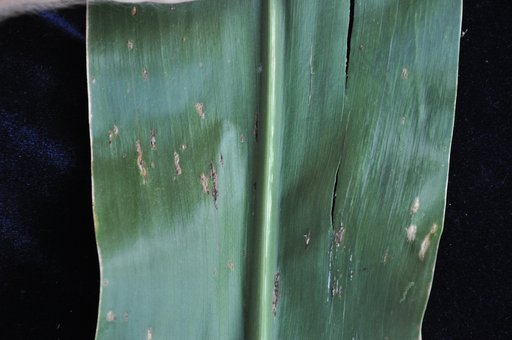
\includegraphics[width=\linewidth]{images/dataset-classes/common_rust.jpg}
\caption*{a) Roya Com\'un}
\end{minipage}
\hfill
\begin{minipage}[b]{0.31\linewidth}
\centering
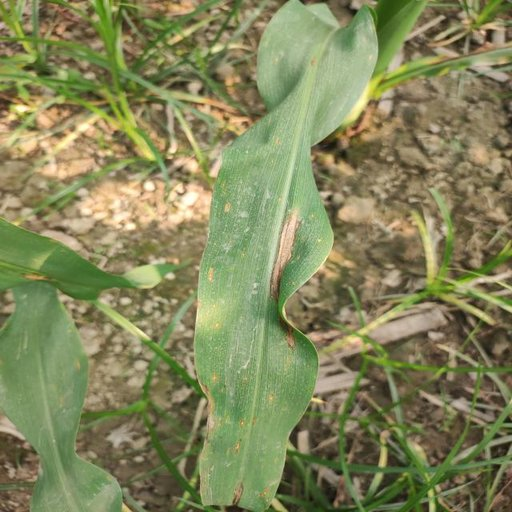
\includegraphics[width=\linewidth]{images/dataset-classes/northern_corn_leaf_blight.jpg}
\caption*{b) Tiz\'on Foliar}
\end{minipage}
\hfill
\begin{minipage}[b]{0.31\linewidth}
\centering
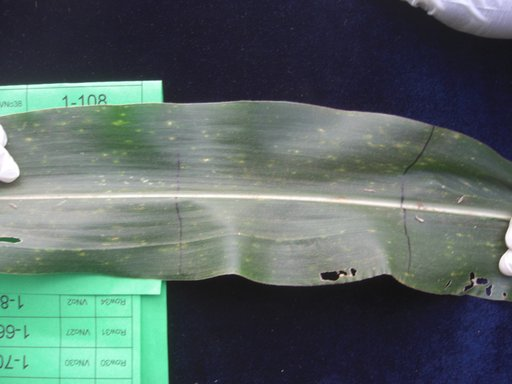
\includegraphics[width=\linewidth]{images/dataset-classes/gray_leaf_spot.jpg}
\caption*{c) Mancha Gris}
\end{minipage}

\vspace{0.3cm}
\begin{minipage}[b]{0.31\linewidth}
\centering
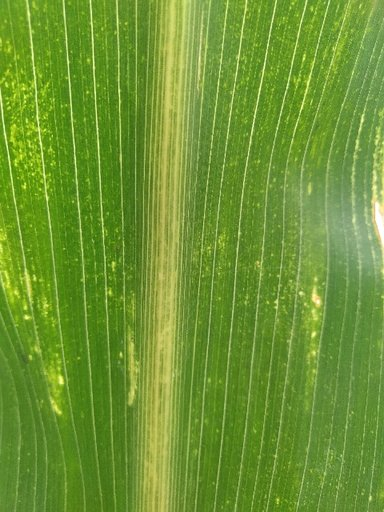
\includegraphics[width=\linewidth]{images/dataset-classes/lethal_necrosis.jpg}
\caption*{d) Necrosis Letal}
\end{minipage}
\hfill
\begin{minipage}[b]{0.31\linewidth}
\centering
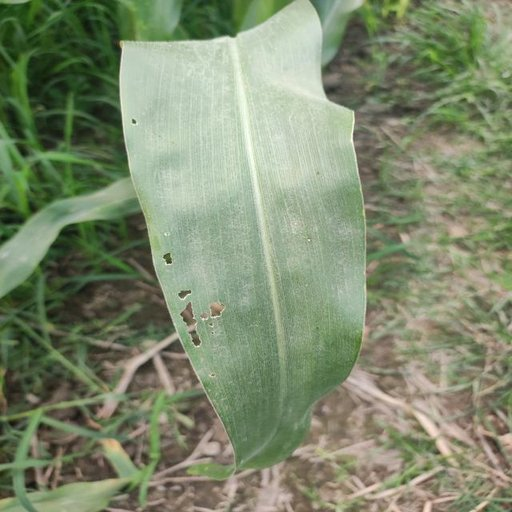
\includegraphics[width=\linewidth]{images/dataset-classes/fall_armyworm.jpg}
\caption*{e) Gusano Cogollero}
\end{minipage}
\hfill
\begin{minipage}[b]{0.31\linewidth}
\centering
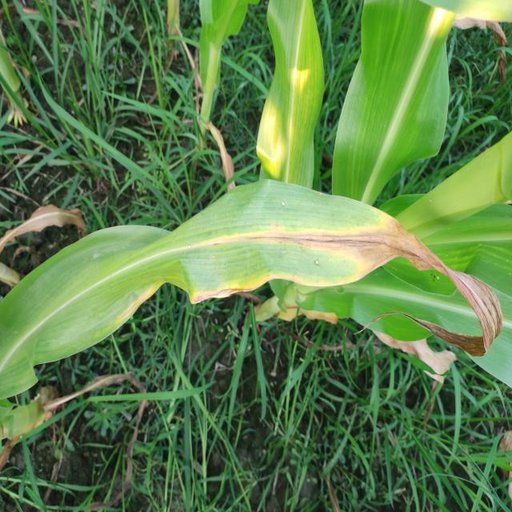
\includegraphics[width=\linewidth]{images/dataset-classes/nitrogen_deficiency.jpg}
\caption*{f) Deficiencia N}
\end{minipage}

\vspace{0.3cm}
\begin{minipage}[b]{0.31\linewidth}
\centering
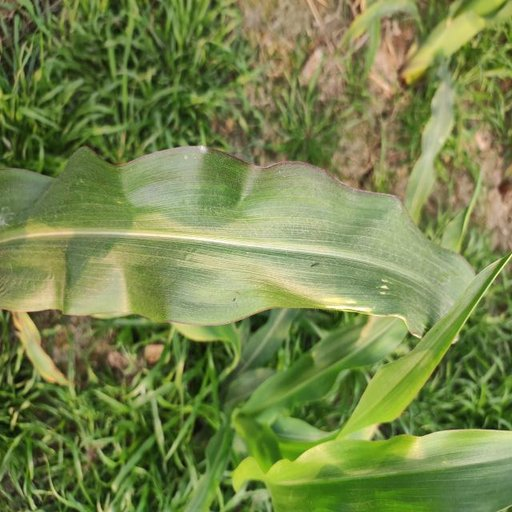
\includegraphics[width=\linewidth]{images/dataset-classes/phosphorus_deficiency.jpg}
\caption*{g) Deficiencia P}
\end{minipage}
\hfill
\begin{minipage}[b]{0.31\linewidth}
\centering
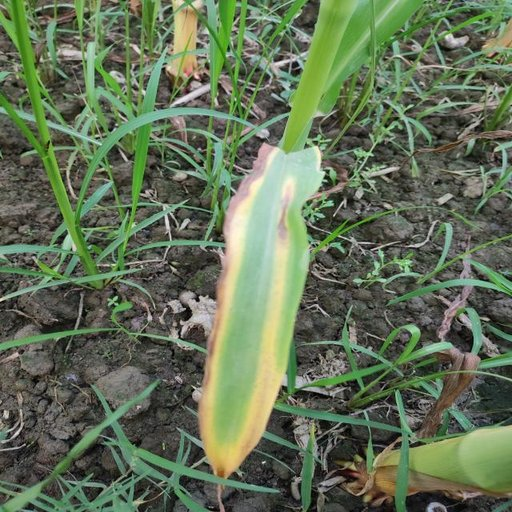
\includegraphics[width=\linewidth]{images/dataset-classes/potassium_deficiency.jpg}
\caption*{h) Deficiencia K}
\end{minipage}
\hfill
\begin{minipage}[b]{0.31\linewidth}
\centering
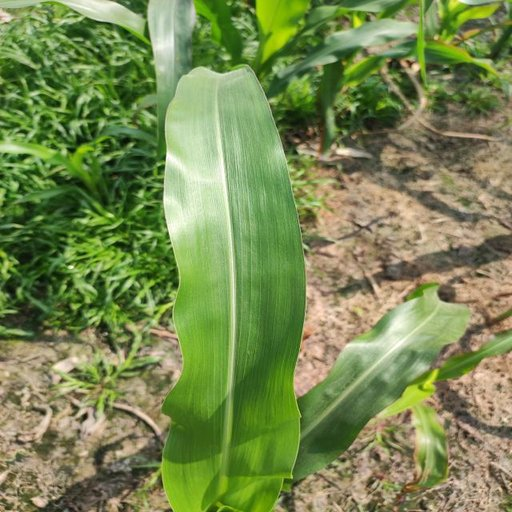
\includegraphics[width=\linewidth]{images/dataset-classes/healthy.jpg}
\caption*{i) Planta Sana}
\end{minipage}
\caption{Cat\'alogo fotogr\'afico de las nueve clases agron\'omicas presentes en el corpus.}
\label{fig:clases_mosaico}
\end{figure}

\section{Recopilaci\'on, Depuraci\'on y Auditor\'ia de Datos}

El corpus final se conform\'o mediante la integraci\'on de \textbf{33~429 im\'agenes elegibles} provenientes de 11 fuentes internacionales consolidadas (Tabla~\ref{tab:fuentes_dataset}). Para resolver el cuello de botella identificado en la primera fase del proyecto —donde la deficiencia de potasio colapsaba a un $F_1$ de 0.49 debido a la escasez extrema de muestras—, se incorporaron cuatro repositorios dirigidos a deficiencias minerales.

\begin{table}[H]
\caption{Fuentes de datos recopiladas y distribuci\'on de muestras}
\label{tab:fuentes_dataset}
\centering
\small
\begin{singlespace}
\begin{tabularx}{\textwidth}{p{6.6cm}ccp{3.6cm}}
\toprule
\textbf{Identificador de Fuente (\texttt{source\_id})} & \textbf{Muestras} & \textbf{Entorno} & \textbf{Patolog\'ias Principales Aportadas} \\
\midrule
\texttt{maize-beans-tomatoes-africa} & 12~136 & Mixto & 4 clases. \\
\texttt{maize-diseases} & 6~989 & Campo Real & 3 clases. \\
\texttt{multicrop-disease-maiz} & 5~816 & Campo Real & 3 clases, incluida necrosis letal (MLN). \\
\texttt{corn-leaf-roboflow} & 2~919 & Mixto & 6 clases. \\
\texttt{cropdg-unified-multidomain} & 2~562 & Mixto & 3 clases. \\
\texttt{maize-in-field-dataset} & 852 & Campo Real & 3 clases. \\
\texttt{maize-2-roboflow} & 846 & Mixto & 3 clases. \\
\texttt{corn-leaf-diseases-}\allowbreak\texttt{classification-roboflow} & 480 & Mixto & 1 clase (\texttt{gray\_leaf\_spot}). \\
\texttt{maize-nutrient-deficiency} & 340 & Mixto & 4 clases. \\
\texttt{maize-leaf-roboflow} & 331 & Mixto & 1 clase. \\
\texttt{maize-deficiency-}\allowbreak\texttt{scanner-roboflow} & 158 & Campo Real & 3 clases de deficiencia. \\
\midrule
\textbf{Total Elegible Auditado} & \textbf{33~429} & — & \textbf{9 clases agron\'omicas} \\
\bottomrule
\end{tabularx}
\end{singlespace}
\end{table}

\subsection{Data Profiling y An\'alisis Exploratorio de Datos (EDA)}
El an\'alisis exploratorio evidenci\'o tres retos estructurales:
\begin{itemize}
\item \textbf{Desbalance intr\'inseco:} La clase sana concentra cerca de 8~700 im\'agenes y el tiz\'on foliar cerca de 6~800, mientras que la deficiencia de potasio cuenta con 621 ejemplares (desbalance de 14.1:1 en el corpus vigente, frente a 32.9:1 antes de la ampliaci\'on).
\item \textbf{Heterogeneidad de resoluci\'on y c\'amaras:} Las resoluciones van desde sensores r\'usticos de $256\times256$ p\'ixeles hasta capturas semiprofesionales de $4000\times3000$ p\'ixeles (Figura~\ref{fig:eda_distribuciones}).
\item \textbf{Asociaci\'on espuria fuente-clase:} La asociaci\'on estad\'istica entre la procedencia y la etiqueta arroj\'o una \textbf{V de Cram\'er de 0.5030}, indicando que ciertas fuentes p\'ublicas aportan exclusivamente una sola patolog\'ia, lo que puede favorecer que las redes utilicen señales del entorno además de la lesión foliar. Esta relación es descriptiva y no establece una causa.
\end{itemize}

\begin{figure}[H]
\centering
\begin{minipage}[b]{0.48\linewidth}
\centering
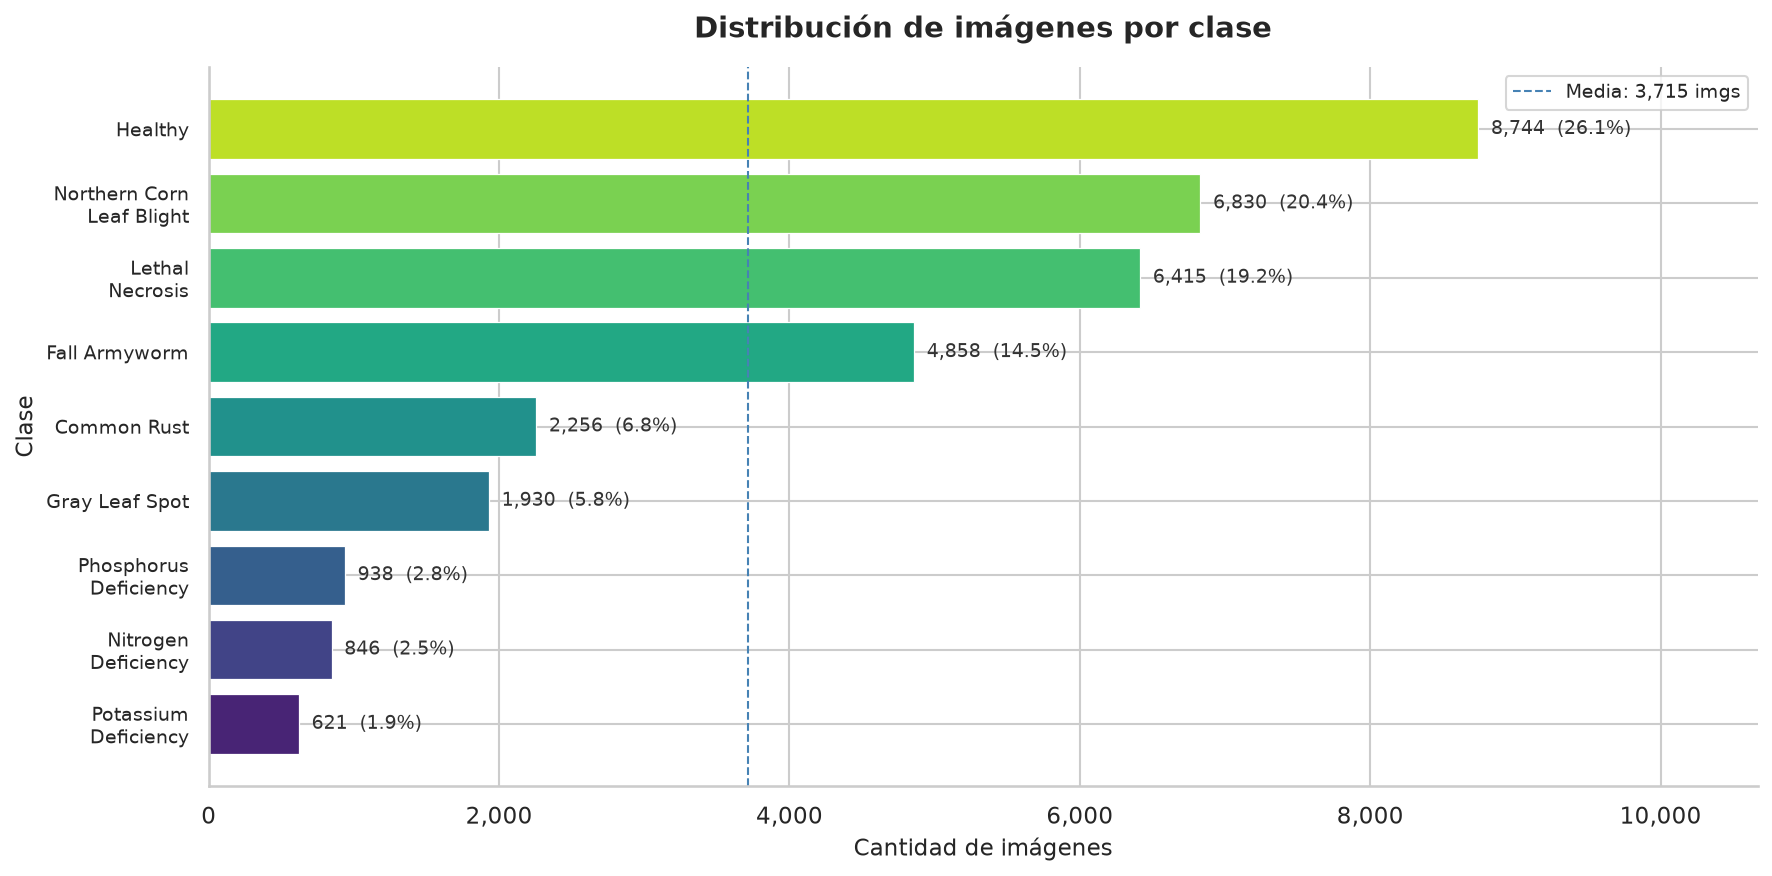
\includegraphics[width=\linewidth]{images/eda/eda_01_distribucion_clases.png}
\caption{Distribuci\'on de muestras por clase.}
\label{fig:eda_clases}
\end{minipage}
\hfill
\begin{minipage}[b]{0.48\linewidth}
\centering
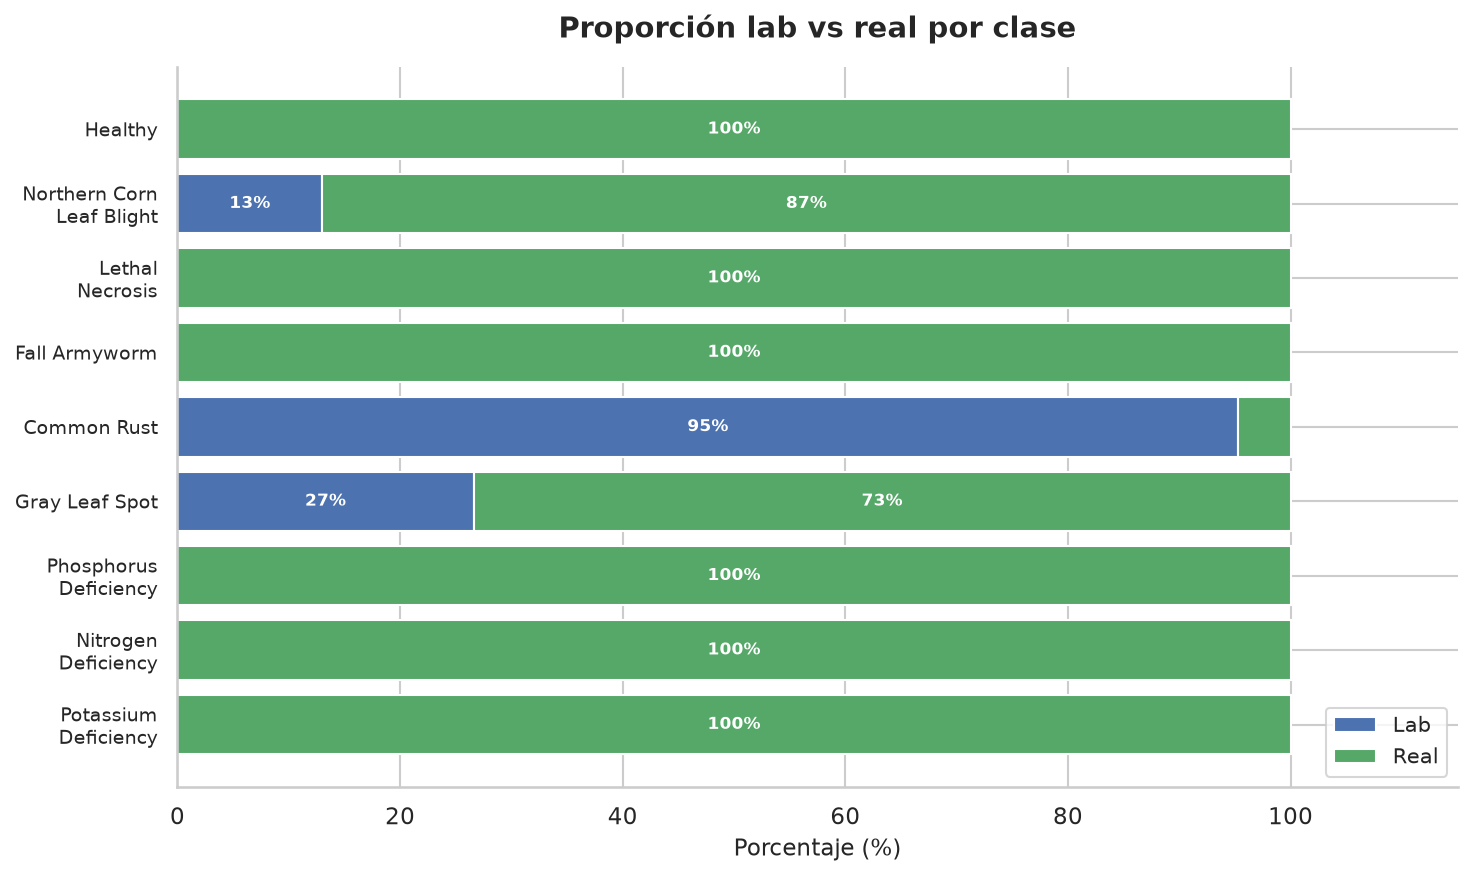
\includegraphics[width=\linewidth]{images/eda/eda_02_lab_vs_real.png}
\caption{Proporci\'on Laboratorio vs. Campo Real.}
\label{fig:eda_lab_real}
\end{minipage}
\caption{An\'alisis exploratorio de distribuci\'on y balance ambiental del corpus.}
\label{fig:eda_distribuciones}
\end{figure}

\begin{figure}[H]
\centering
\begin{minipage}[b]{0.48\linewidth}
\centering
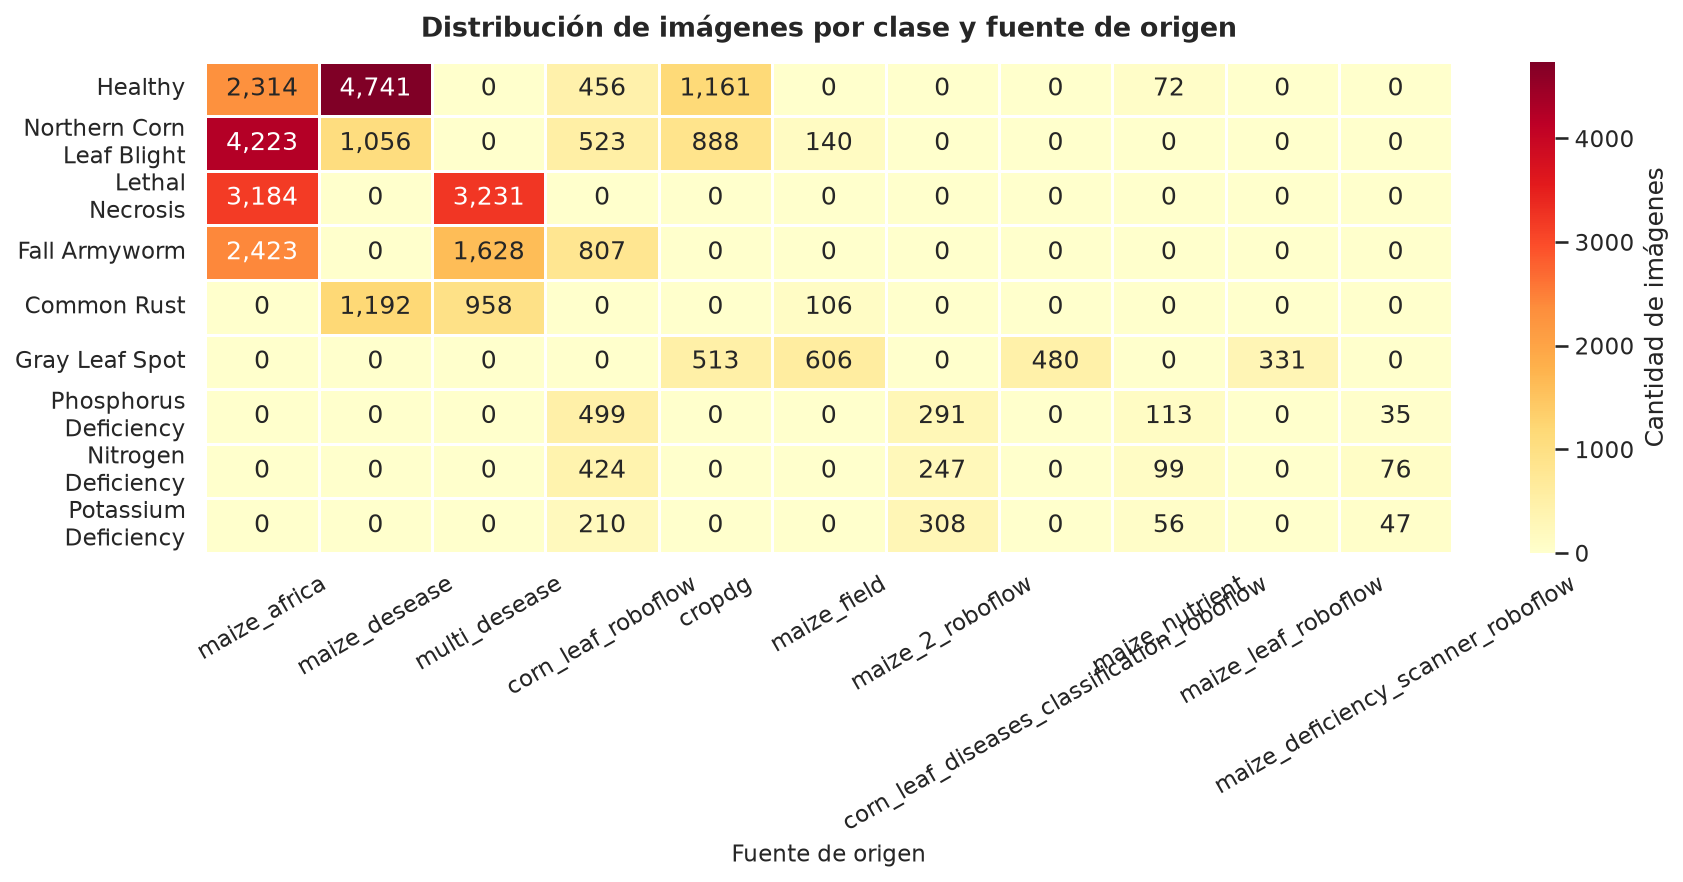
\includegraphics[width=\linewidth]{images/eda/eda_02b_heatmap_fuente_clase.png}
\caption{Matriz de contingencia fuente vs. patolog\'ia.}
\label{fig:eda_heatmap}
\end{minipage}
\hfill
\begin{minipage}[b]{0.48\linewidth}
\centering
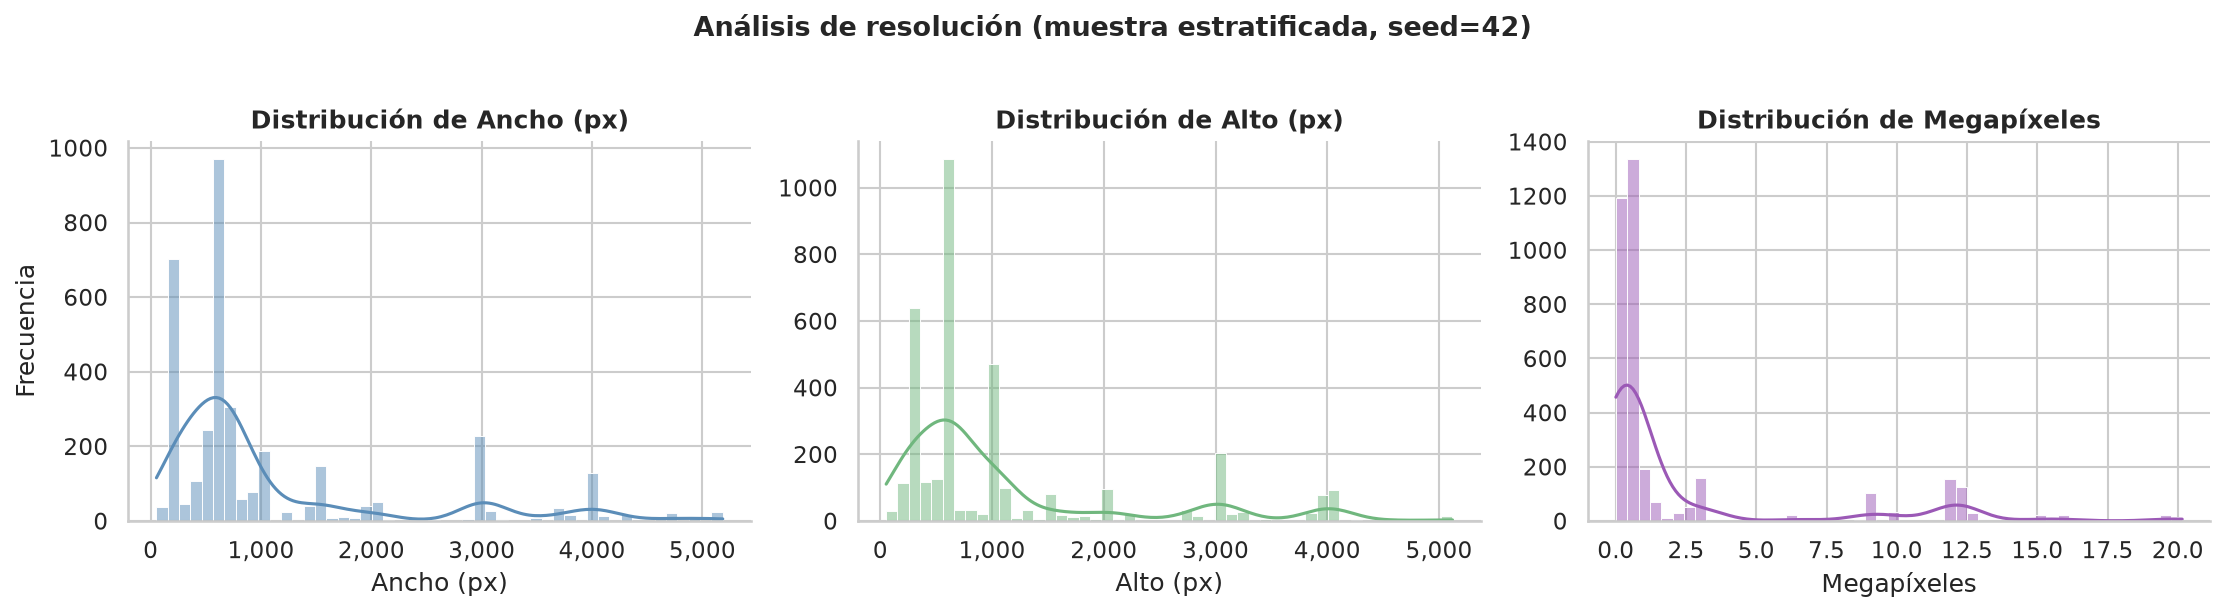
\includegraphics[width=\linewidth]{images/eda/eda_03_resoluciones.png}
\caption{Distribuci\'on de resoluciones espaciales.}
\label{fig:eda_resoluciones}
\end{minipage}
\caption{Concentraci\'on de procedencia y heterogeneidad geom\'etrica en las im\'agenes.}
\end{figure}

\subsection{Auditor\'ia Criptogr\'afica de P\'ixeles}
Para descartar que la precisi\'on reportada se inflara por duplicados id\'enticos en entrenamiento y prueba, se ejecut\'o la auditor\'ia \texttt{PIXEL\_DUPLICATE\_AUDIT}. Se calcularon hashes SHA-256 directos sobre el contenido decodificado en memoria. Se descubrieron \'unicamente cuatro grupos de im\'agenes (ocho archivos en total) con etiquetas contradictorias entre repositorios, los cuales fueron purgados de inmediato. Las \textbf{33~429 muestras finales no presentan un solo duplicado id\'entico cross-split}.

La partici\'on de desarrollo oficial (\texttt{seed\_42}) qued\'o estructurada en un reparto estratificado 70/15/15:
\begin{itemize}
\item \textbf{Entrenamiento:} 23~400 im\'agenes.
\item \textbf{Validaci\'on:} 5~014 im\'agenes.
\item \textbf{Prueba independiente (Test retenido):} 5~015 im\'agenes.
\end{itemize}

\noindent\textbf{Limitaci\'on de la partici\'on de desarrollo.} La partici\'on \texttt{seed\_42} es estratificada por \texttt{label + environment} y mezcla las fuentes conocidas entre entrenamiento, validaci\'on y prueba. Esta configuraci\'on es adecuada para desarrollo \textit{in-distribution}, pero no demuestra generalizaci\'on a una c\'amara, parcela o repositorio nuevo. Adem\'as, la materializaci\'on se gener\'o con \texttt{deduplicate\_perceptual=false}, por lo que la posible fuga por im\'agenes casi duplicadas no fue medida en este trabajo. La evaluaci\'on agrupada por fuente y el estudio \textit{leave-one-source-out} se presentan en el cap\'itulo de resultados.

\section{Arquitecturas y B\'usqueda de Hiperpar\'ametros}

\subsection{Familias Convolucionales Seleccionadas}
Se seleccionaron tres redes convolucionales modernas de alta eficiencia, representativas de diversas hip\'otesis inductivas:
\begin{enumerate}
\item \textbf{EfficientNet-Lite0 (Modelo m\'ovil desplegado):} Variante dise\~nada espec\'ificamente para inferencia m\'ovil y cuantizaci\'on. Elimina las activaciones no lineales complejas (\textit{swish}) sustituy\'endolas por ReLU6, y suprime los bloques de atenci\'on \textit{Squeeze-and-Excitation} (SE) \cite{hu2018} para mantener compatibilidad plena con aceleradores de enteros (3.38 millones de par\'ametros) \cite{tan2019}.
\item \textbf{EfficientNet-B0 (Referencia de capacidad):} Arquitectura balanceada con escalado compuesto y bloques SE con atenci\'on por canal (4.02 millones de par\'ametros).
\item \textbf{ShuffleNet-V2-x1.0 (Eficiencia extrema):} Basada en divisi\'on de canales (\textit{Channel Split}) y barajado (\textit{Channel Shuffle}) para maximizar el flujo de informaci\'on minimizando los accesos a memoria DRAM (1.26 millones de par\'ametros) \cite{ma2018}.
\end{enumerate}

\subsection{Espacio de B\'usqueda y Poda Temprana}
La optimizaci\'on de hiperpar\'ametros se formul\'o mediante un estudio bayesiano en \textbf{Optuna} \cite{optuna2019} con el estimador de \'arbol de Parzen multivariado (TPE). La funci\'on objetivo maximiz\'o el Macro $F_1$ sobre el conjunto de validaci\'on oficial. Para no desperdiciar horas de GPU en configuraciones no prometedoras, se incorpor\'o el algoritmo \textbf{MedianPruner}: a partir de la \'epoca 8 (periodo de calentamiento), si el Macro $F_1$ de un ensayo se sit\'ua por debajo de la mediana hist\'orica de los ensayos precedentes, el entrenamiento se detiene autom\'aticamente (\textit{PRUNED}).

El espacio de exploraci\'on abarc\'o siete par\'ametros cr\'iticos (Tabla~\ref{tab:hpo_espacio}).

\begin{table}[H]
\caption{Espacio de b\'usqueda de hiperpar\'ametros explorado con Optuna}
\label{tab:hpo_espacio}
\centering
\small
\begin{singlespace}
\begin{tabularx}{\textwidth}{lp{4.2cm}X}
\toprule
\textbf{Hiperpar\'ametro} & \textbf{Rango / Opciones} & \textbf{Fundamento Ingenieril} \\
\midrule
\texttt{learning\_rate} & Log-uniforme: $[10^{-5}, 3\times10^{-3}]$ & Control de convergencia en optimizador AdamW. \\
\texttt{batch\_size} & Categ\'orico: $\{16, 32, 64\}$ & Estabilidad del gradiente estoc\'astico y saturaci\'on de GPU. \\
\texttt{weight\_decay} & Log-uniforme: $[10^{-6}, 10^{-2}]$ & Regularizaci\'on $L_2$ para mitigar memorizaci\'on de fondos. \\
\texttt{class\_weights} & $\{\text{none}, \text{inv}, \text{sqrt\_inv}\}$ & Ponderaci\'on de p\'erdida para compensar desbalance de clases. \\
\texttt{label\_smoothing} & Uniforme: $[0.0, 0.15]$ & Calibraci\'on probabil\'istica y prevenci\'on de sobreconfianza. \\
\texttt{warmup\_epochs} & Entero: $[1, 5]$ & Calentamiento lineal para proteger pesos preentrenados. \\
\texttt{clahe} & Fijo en \texttt{False} & Ecualizaci\'on adaptativa excluida de la b\'usqueda; se evalu\'o aparte. \\
\bottomrule
\end{tabularx}
\end{singlespace}
\end{table}

\subsection{Ensamble Multimodelo por Soft Voting}
Para mitigar el riesgo de diagn\'osticos err\'oneos causados por las zonas ciegas de una sola arquitectura, se implement\'o un ensamble heterog\'eneo por votaci\'on suave. El ensamble calcula el vector de probabilidades promedio:
\begin{equation}
P_{\text{ens}}(y = c \mid x) = \frac{1}{M} \sum_{m=1}^{M} P_m(y = c \mid x)
\end{equation}
donde $M=3$ corresponde a las tres redes entrenadas independientemente y $c \in \{1, \dots, 9\}$. La decisi\'on final se obtiene por consenso m\'aximo: $\hat{y} = \arg\max_c P_{\text{ens}}(y = c \mid x)$.

\section{Despliegue en Dispositivo M\'ovil}

\subsection{Cuantizaci\'on a Enteros de 8 Bits (Int8)}
Para permitir que \texttt{EfficientNet-Lite0} opere en tel\'efonos sin unidad de procesamiento neuronal (\textit{NPU}), se realiz\'o una cuantizaci\'on posterior al entrenamiento (\textit{Post-Training Quantization}, PTQ) \cite{jacob2018} hacia enteros de 8 bits, exportando el modelo mediante litert-torch. El esquema es simétrico (punto cero $Z = 0$) y dinámico: las escalas de activación se calculan en tiempo de ejecución, por lo que no requiere un conjunto de calibración. En el backbone, cada canal de salida $c$ tiene su propia escala $S_c$, que mapea los pesos en coma flotante $W_{f,c,i}$ a enteros con signo:
\begin{equation}
S_c = \frac{\max_i \lvert W_{f,c,i} \rvert}{127}, \qquad q_{c,i} = \operatorname{clip}\!\left(\left\lfloor \frac{W_{f,c,i}}{S_c} \right\rceil,\; -127,\; 127\right)
\end{equation}
La capa lineal final usa una \'unica escala por tensor, porque el kernel de TFLite para \texttt{FULLY\_CONNECTED} dinámico aplica una sola escala. Con escalas por canal, los logits de esa capa quedan multiplicados por una constante distinta por clase sin que el runtime lo señale. Cuantizar todas las capas por tensor, en cambio, degrada las convoluciones \textit{depthwise} de EfficientNet, cuyos pesos tienen rangos muy distintos entre canales; por ello el backbone se cuantiza por canal. La operaci\'on permite que las multiplicaciones de matrices de convoluci\'on se resuelvan con instrucciones vectoriales enteras en la CPU m\'ovil. El consumo energ\'etico no fue medido en este trabajo.

\subsection{Detector de Anomal\'ias Fuera de Distribuci\'on (OOD)}
Las redes neuronales pueden emitir clasificaciones con alta confianza cuando reciben im\'agenes que no pertenecen a ninguna de sus clases, por ejemplo suelo, calzado o malezas, porque la confianza softmax solo mide la elecci\'on entre las etiquetas conocidas \cite{lee2018}. Para detectar este caso, DoctorMaiz extrae el vector de activaci\'on de la capa previa a la clasificaci\'on ($d = 1~280$ dimensiones), reduce su dimensionalidad mediante PCA a 186 componentes que retienen el 99\,\% de la varianza y eval\'ua la \textbf{Distancia Relativa de Mahalanobis (RMD)} \cite{ren2021}. La distancia resta un modelo de fondo global para no penalizar caracter\'isticas gen\'ericas de cualquier fotograf\'ia:
El vector se normaliza a norma L2 unitaria antes de proyectarlo \cite{mahalanobispp2025}. La puntuaci\'on es
\begin{equation}
\text{RMD}(z) = D_M\!\left(z \,\middle|\, \mu_{c^*}, \Sigma\right) - D_M\!\left(z \,\middle|\, \mu_0, \Sigma_0\right)
\end{equation}
donde $\mu_{c^*}$ es el centroide de la clase m\'as cercana, $\Sigma$ es la covarianza agrupada entre clases y $\mu_0$, $\Sigma_0$ describen una gaussiana de fondo sobre todo el conjunto de entrenamiento. Ambas covarianzas se regularizan con un t\'ermino ridge proporcional a su traza antes de invertirlas.

El umbral se calibra sobre el conjunto de validaci\'on, no visto durante el entrenamiento, como el percentil 95 de la puntuaci\'on de cada hoja v\'alida. El umbral de la aplicaci\'on instalada est\'a pendiente de regeneraci\'on: el archivo de estad\'isticas OOD que empaqueta la aplicaci\'on no tiene un run de origen registrado. El modelo instalado corresponde al run \texttt{20260812\_221429} (SHA-256 del \texttt{.tflite} verificado), pero su archivo \texttt{ood\_stats.json} no existe en la exportaci\'on de ese run. El valor se obtendr\'a al ejecutar \texttt{compute\_ood\_stats.py} sobre dicho checkpoint. Las pruebas sint\'eticas (pantallas negras, ruido aleatorio) superaron valores de 300 y las fotograf\'ias reales de campo quedaron por debajo del umbral. Si la puntuaci\'on supera el umbral, la aplicaci\'on muestra la advertencia \textbf{«Imagen no reconocida»} y no emite diagn\'ostico.

\subsection{Mitigaci\'on en la Interfaz: Marco Gu\'ia y Severidad}
Como se demostrar\'a en el cap\'itulo de resultados, el software no puede eliminar por completo los atajos de fondo de los repositorios p\'ublicos. Por ello, la soluci\'on integr\'o dos innovaciones directas en la aplicaci\'on:
\begin{enumerate}
\item \textbf{C\'amara con marco gu\'ia foliar y recorte autom\'atico:} La interfaz superpone una silueta ergon\'omica de la hoja con la instrucci\'on expl\'icita: \textit{«Ac\'erquese a 20--30 cm y llene el marco»}. La aplicaci\'on recorta la imagen capturada a la regi\'on delimitada por el marco gu\'ia antes de pasar la matriz al modelo, de modo que el \'area enviada corresponde a la hoja y no al entorno completo.
\item \textbf{Gu\'ia de severidad en lenguaje campesino:} Dado que los modelos de clasificaci\'on no pueden predecir el porcentaje de \'area foliar comprometida, la app despliega debajo de la etiqueta una escala visual de tres niveles (baja, moderada, cr\'itica) basada en manuales homologados del CIMMYT e Iowa State, descrita en t\'erminos coloquiales y recomendando bioinsumos accesibles en el agroservicio local.
\end{enumerate}

\section{Segmentaci\'on de Hojas: dos usos y resultados}

El proyecto utiliz\'o la segmentaci\'on foliar en dos l\'ineas distintas, con evidencia y estado diferentes. Ninguna de ellas forma parte de la predicci\'on de la aplicaci\'on instalada, que recorta geom\'etricamente la imagen con el marco gu\'ia.

	extbf{Primer uso: presegmentaci\'on y entrenamiento sobre corpus enmascarado.} El pipeline del clasificador incluye un m\'odulo de segmentaci\'on (	exttt{src/segmentation}) que genera un corpus con m\'ascaras de hoja. Se entren\'o un modelo sobre ese corpus (run 	exttt{20260907\_163546}, EfficientNet-Lite0, sobre el split 	exttt{seed\_42\_segmented}). Su Macro $F_1$ en prueba fue de 	extbf{0.7191} y su accuracy de 0.8903, frente a 0.9480 del baseline de imagen completa vigente. Esta comparaci\'on no es pareada: el conjunto de prueba segmentado no comparte ninguna imagen con el conjunto de prueba original (0 de 5~015 rutas coinciden). El perfil de m\'ascara usado para generar el corpus no est\'a registrado en el resumen del run, por lo que el resultado no permite atribuir la ca\'ida a un perfil concreto. El proyecto clasifica este uso como experimental y no como preprocesamiento general.

	extbf{Segundo uso: segmentador de instancias para aislar la hoja.} En un repositorio independiente se entren\'o un segmentador YOLO (	exttt{yolo26n-seg}, Ultralytics 8.4.104) para seleccionar la hoja principal. La configuraci\'on D-01 cambi\'o un solo hiperpar\'ametro (	exttt{mosaic=0}) sobre la configuraci\'on base de semilla 42 y se evalu\'o \'unicamente sobre validaci\'on. Obtuvo 	extit{Mask mAP50-95} de 0.94404 y 	extit{Mask recall} de 0.94309. Sobre 150 hojas enfermas de validaci\'on, el quality gate marc\'o 150 m\'ascaras como 	exttt{reliable}, con IoU medio de 0.98122 y Dice medio de 0.99046. Estos resultados son de una sola semilla y no incluyen evaluaci\'on sobre el conjunto de prueba ni sobre el piloto de fuente externa, que siguen sin ejecutarse.

La implicaci\'on para el dise\'no es que una m\'ascara puede eliminar se\~nal \'util del fondo. Por ello el proyecto no aplica segmentaci\'on de forma universal, y la comparaci\'on formal entre imagen completa y segmentada sigue pendiente.


\section{Sincronizaci\'on y Contribuci\'on al Dataset Colaborativo}

La aplicaci\'on funciona sin servidor. Esta secci\'on describe el dise\~no de la sincronizaci\'on opcional, implementado en el repositorio de la API. Su comportamiento descrito aqu\'i proviene del c\'odigo y de la especificaci\'on de dise\~no; las pruebas de integraci\'on previstas en esa especificaci\'on no se han ejecutado en este trabajo.

El dise\~no contempla dos tipos de registro que la aplicaci\'on env\'ia cuando hay conexi\'on y una cuenta registrada: correcciones de diagn\'ostico y aportes fotogr\'aficos al dataset colaborativo. Ambos se almacenan en MySQL 8.4 y no se incluye telemetr\'ia de escaneos ni coordenadas GPS del historial.

Los dos endpoints de escritura son \texttt{POST /corrections} y \texttt{POST /dataset-contributions}. La especificaci\'on define que ambos sean idempotentes por el par \texttt{(user\_id, client\_id)}: un reenv\'io con el mismo identificador debe devolver el registro existente en lugar de duplicarlo. Tambi\'en define un l\'imite de 30 solicitudes por minuto por usuario autenticado. El env\'io de imagen se valida como archivo de imagen antes de guardarse. Estas tres propiedades son de dise\~no; su verificaci\'on queda pendiente.

El env\'io previsto incluye la fotograf\'ia, la etiqueta elegida, una nota opcional y la fecha del escaneo. No incluye nombre, tel\'efono, correo ni coordenadas GPS. La aplicaci\'on no elimina los metadatos EXIF de la fotograf\'ia antes de enviarla, por lo que este punto queda como pendiente de tratamiento.

Sin cuenta registrada, la aplicaci\'on conserva los aportes en el tel\'efono y no los env\'ia. La cola de sincronizaci\'on reintenta cuando hay conexi\'on.

\subsection{Modelo relacional de la base de datos del servidor}

El servidor almacena cinco tablas en MySQL 8.4, definidas en la migración inicial de Alembic. La Figura~\ref{fig:er_api} muestra sus relaciones. La única dependencia entre tablas es que cada registro de usuario agrupa sus tokens de sesión y sus aportes, y la tabla de versiones de la aplicación no se relaciona con las demás.

\begin{figure}[H]
\centering
\begin{tikzpicture}[
  ent/.style={draw=blue!55!black, fill=blue!4, rounded corners=2pt, align=left, font=\scriptsize, inner sep=4pt, text width=4.2cm},
  rel/.style={-{Latex[length=2.2mm]}, line width=0.8pt, draw=gray!70}
]
\node[ent] (users) {\textbf{users}\\[1pt]
  id \emph{(PK)}\\ name, email \emph{(único)}\\ password\_hash, created\_at};
\node[ent, below=1.1cm of users, xshift=-5.6cm] (rt) {\textbf{refresh\_tokens}\\[1pt]
  id \emph{(PK)}\\ user\_id \emph{(FK)}\\ token\_hash \emph{(único)}, expires\_at, revoked\_at, created\_at};
\node[ent, below=1.1cm of users, xshift=0cm] (corr) {\textbf{corrections}\\[1pt]
  id \emph{(PK)}\\ user\_id \emph{(FK)}, client\_id\\ scan\_id, observed\_label, note, status\\ created\_at, received\_at\\ \emph{único:} (user\_id, client\_id)};
\node[ent, below=1.1cm of users, xshift=5.6cm] (dc) {\textbf{dataset\_contributions}\\[1pt]
  id \emph{(PK)}\\ user\_id \emph{(FK)}, client\_id\\ image\_path, label, note, status\\ created\_at, received\_at\\ \emph{único:} (user\_id, client\_id)};
\node[ent, below=5.2cm of users, xshift=0cm] (ar) {\textbf{app\_releases}\\[1pt]
  id \emph{(PK)}\\ platform, version\_code, version\_name\\ min\_supported\_version\_code\\ download\_url, release\_notes\\ published\_at, is\_active};
\draw[rel] (users.south west) -- ++(0,-0.4) -| (rt.north);
\draw[rel] (users.south) -- (corr.north);
\draw[rel] (users.south east) -- ++(0,-0.4) -| (dc.north);
\end{tikzpicture}
\caption{Modelo relacional del servidor. Las flechas van de \texttt{users} a las tablas que referencian su \texttt{id}. \texttt{app\_releases} no tiene relaciones.}
\label{fig:er_api}
\end{figure}

\subsection{Flujo de sincronizaci\'on desde la aplicaci\'on}

La Figura~\ref{fig:secuencia_sync} describe el recorrido de un aporte desde que el productor lo guarda hasta que el servidor lo confirma. El guardado es local e inmediato. La sincronizaci\'on se dispara al recuperar la red o por acci\'on del usuario, y antes de enviar comprueba en orden tres condiciones: que existan registros pendientes, que haya conexi\'on y que haya una sesi\'on. Si no hay pendientes, el proceso termina sin enviar nada. Si el servidor responde 401, la aplicaci\'on refresca el token una sola vez y reintenta. Un registro solo se marca como sincronizado tras la confirmaci\'on del servidor; si el env\'io falla, permanece pendiente para el siguiente intento.

\begin{figure}[H]
\centering
\begin{tikzpicture}[
  life/.style={draw=gray!60, line width=0.5pt, dashed},
  pt/.style={draw=blue!55!black, fill=blue!5, rounded corners=2pt, align=center, font=\scriptsize, minimum height=0.7cm, minimum width=2.4cm},
  msg/.style={-{Latex[length=2mm]}, line width=0.7pt},
  rmsg/.style={-{Latex[length=2mm]}, line width=0.7pt, dashed},
  self/.style={font=\tiny, align=left, draw=gray!50, fill=yellow!8, rounded corners=1pt, inner sep=2pt},
  lab/.style={font=\tiny, fill=white, inner sep=1pt}
]
\def\yp{0}
\node[pt] (P) at (0,0) {Productor};
\node[pt] (A) at (3.4,0) {App DoctorMaiz};
\node[pt] (D) at (6.8,0) {SQLite local};
\node[pt] (S) at (10.2,0) {Servidor (API)};
\draw[life] (P) -- (0,-9.2);
\draw[life] (A) -- (3.4,-9.2);
\draw[life] (D) -- (6.8,-9.2);
\draw[life] (S) -- (10.2,-9.2);

% 1 productor -> app : toma foto
\draw[msg] (0,-0.9) -- (3.4,-0.9) node[midway, lab, above] {1. Toma foto};
% 2 app -> sqlite : guarda pendiente
\draw[msg] (3.4,-1.6) -- (6.8,-1.6) node[midway, lab, above] {2. Guarda aporte pendiente};
% 3 confirmacion local
\draw[rmsg] (6.8,-2.1) -- (3.4,-2.1) node[midway, lab, above] {3. Confirmaci\'on local};

% 4 self: disparo
\draw[self] (3.4,-2.8) -- (3.4,-2.8);
\node[self, anchor=west] at (3.6,-2.9) {4. Disparo: cambio de red o bot\'on};

% 5 app -> sqlite : hay pendientes
\draw[msg] (3.4,-3.6) -- (6.8,-3.6) node[midway, lab, above] {5. \'Hay pendientes?};
% 6 respuesta
\draw[rmsg] (6.8,-4.1) -- (3.4,-4.1) node[midway, lab, above] {6. No: termina sin enviar};

% 6b alternative pending yes continues (self note)
\node[self, anchor=west] at (3.6,-4.8) {7. S\'i: comprueba red (NetInfo) y sesi\'on};

% 7 app -> servidor : POST sin token valido
\draw[msg] (3.4,-5.6) -- (10.2,-5.6) node[midway, lab, above] {8. POST aporte};
% 8 servidor -> app : 401
\draw[rmsg] (10.2,-6.1) -- (3.4,-6.1) node[midway, lab, above] {9. 401 si no hay sesi\'on};
% 9 refresh and retry
\draw[msg] (3.4,-6.6) -- (10.2,-6.6) node[midway, lab, above] {10. Refresca token y reintenta};
% 10 ack
\draw[rmsg] (10.2,-7.1) -- (3.4,-7.1) node[midway, lab, above] {11. 201 o 200 (confirmaci\'on)};
% 11 marca synced
\draw[msg] (3.4,-7.7) -- (6.8,-7.7) node[midway, lab, above] {12. Marca synced = true};

% failure branch note
\node[self, anchor=west] at (3.6,-8.4) {Si el env\'io falla: el registro queda pendiente};
\end{tikzpicture}
\caption{Flujo de sincronizaci\'on de un aporte, desde el guardado local hasta la confirmaci\'on del servidor. Si el env\'io falla, el registro permanece pendiente.}
\label{fig:secuencia_sync}
\end{figure}

\section{Arquitectura General del Sistema}

\subsection{Tecnolog\'ias por proyecto}

El sistema se compone de cuatro repositorios independientes. La Tabla~\ref{tab:tecnologias_c2} resume la pila tecnol\'ogica de cada uno, con las versiones fijadas en sus archivos de dependencias.

\begin{table}[H]
\caption{Tecnolog\'ias principales por proyecto}
\label{tab:tecnologias_c2}
\centering
\small
\begin{singlespace}
\begin{tabularx}{\textwidth}{>{\raggedright\arraybackslash}p{3.2cm}>{\raggedright\arraybackslash}p{4.2cm}X}
\toprule
\textbf{Proyecto} & \textbf{Funci\'on} & \textbf{Tecnolog\'ias} \\
\midrule
Pipeline del modelo & Entrenamiento, exportaci\'on y explicabilidad & PyTorch (\texttt{torch} 2.4 a 2.12), timm, Optuna, litert-torch y ONNX Runtime para exportaci\'on, Modal (GPU A10) para entrenamiento en la nube, SHAP y LIME. \\
Aplicaci\'on m\'ovil & Captura, inferencia local y sincronizaci\'on & Expo 57, React Native 0.86, TypeScript 6, \texttt{react-native-fast-tflite} 3 para inferencia, WatermelonDB 0.28 con SQLite local, NativeWind 4. \\
API de sincronizaci\'on & Versi\'on de la app y aportes al dataset colaborativo & FastAPI 0.115, SQLAlchemy 2.0, Alembic 1.13, MySQL 8.4 en Docker Compose, aiomysql, JWT y bcrypt para autenticaci\'on, slowapi para l\'imites de tasa. \\
Segmentador de hojas & Aislamiento de la l\'amina foliar (experimental) & Ultralytics 8.4.104 con modelo \texttt{yolo26n-seg}, PyTorch 2.2 a 2.12, Modal para entrenamiento, Pillow y NumPy. \\
\bottomrule
\end{tabularx}
\end{singlespace}
\end{table}

La separaci\'on en repositorios tiene una consecuencia pr\'actica: la aplicaci\'on no depende del entorno de entrenamiento. Solo consume un archivo \texttt{.tflite}, un \texttt{labels.json} y un \texttt{ood\_stats.json} empaquetados. La API y la aplicaci\'on se comunican por HTTP y MySQL solo existe en el servidor.


La Figura~\ref{fig:arquitectura_flujo} sintetiza la arquitectura de extremo a extremo que conecta la fase de experimentaci\'on con el despliegue m\'ovil y la extensi\'on institucional.

\begin{figure}[H]
\centering
\begin{tikzpicture}[
    node distance=0.7cm and 0.9cm,
    stage/.style={
        rectangle, rounded corners=4pt, draw=gray!50, line width=0.8pt,
        minimum width=2.9cm, minimum height=1.35cm, text width=2.7cm,
        align=center, font=\footnotesize, fill=gray!4
    },
    phase/.style={font=\scriptsize\bfseries\itshape, text=gray!60!black},
    arrow/.style={-{Latex[length=2.8mm]}, line width=1pt, draw=gray!60}
]
% --- Fila 1: entrenamiento ---
\node[phase] (lbl1) {Fase de entrenamiento y selecci\'on};
\node[stage, fill=blue!6, draw=blue!55!black, below=0.35cm of lbl1, xshift=-3.3cm] (datos)
  {\textbf{Fuentes p\'ublicas}\\[2pt]33~429 im\'agenes\\11 fuentes};
\node[stage, fill=blue!6, draw=blue!55!black, right=of datos] (pipe)
  {\textbf{Pipeline MLOps}\\[2pt]Deduplicaci\'on\\y contratos};
\node[stage, fill=blue!6, draw=blue!55!black, right=of pipe] (optuna)
  {\textbf{Optuna en GPU}\\[2pt]Poda temprana\\(25 intentos)};
\node[stage, fill=blue!6, draw=blue!55!black, right=of optuna] (lite0)
  {\textbf{EfficientNet-Lite0}\\[2pt]Configuraci\'on oficial\\[2pt]{\scriptsize run 20260921}};
\draw[arrow] (datos) -- (pipe);
\draw[arrow] (pipe) -- (optuna);
\draw[arrow] (optuna) -- (lite0);

% --- Fila 2: despliegue ---
\node[phase, below=1.3cm of datos, xshift=1.2cm] (lbl2) {Fase de despliegue m\'ovil};
\node[stage, fill=green!6, draw=green!45!black, below=0.35cm of lbl2, xshift=-3.3cm] (quant)
  {\textbf{Cuantizaci\'on Int8}\\[2pt]PTQ con litert-torch\\(3.56~MB)};
\node[stage, fill=green!6, draw=green!45!black, right=of quant] (app)
  {\textbf{App DoctorMaiz}\\[2pt]React Native\\y Fast-TFLite};
\node[stage, fill=green!6, draw=green!45!black, right=of app] (ood)
  {\textbf{Captura y OOD}\\[2pt]Marco gu\'ia y\\distancia RMD};
\node[stage, fill=green!6, draw=green!45!black, right=of ood] (off)
  {\textbf{Inferencia local}\\[2pt]CPU, sin conexi\'on\\(sincronizaci\'on opcional)};
\draw[arrow] (quant) -- (app);
\draw[arrow] (app) -- (ood);
\draw[arrow] (ood) -- (off);

% --- Conexi\'on entre filas ---
\draw[arrow, dashed] (lite0.south) |- ++(0,-0.55) -| (quant.north);
\end{tikzpicture}
\caption{Diagrama de flujo arquitect\'onico integral del sistema DoctorMaiz.}
\label{fig:arquitectura_flujo}
\end{figure}

\chapter{Estrategia de Implementaci\'on y An\'alisis de Resultados}

\section{Estrategia y Entorno de Implementaci\'on}

El desarrollo computacional del proyecto se articul\'o en una arquitectura h\'ibrida que desacopla la fase de entrenamiento a gran escala en la nube (\textit{Cloud Training}) de la fase de operaci\'on local en el tel\'efono (\textit{Edge Inference}).

\subsection{Infraestructura de C\'omputo y Entrenamiento en la Nube}
Los modelos se entrenaron sobre instancias aceleradas por hardware en la plataforma Modal, empleando unidades de procesamiento gr\'afico \textbf{NVIDIA A10G} (24~GB VRAM GDDR6, 125 TFLOPS de rendimiento tensorial) montadas sobre entornos Linux con CUDA 12.1 y PyTorch 2.3. Se aplic\'o precisi\'on mixta autom\'atica (\textit{AMP bfloat16}) para maximizar el ancho de banda y la saturaci\'on de memoria.

El r\'egimen de entrenamiento incorpor\'o un programador de tasa de aprendizaje por recocido cosenoidal con calentamiento lineal (\textit{Cosine Annealing with Warmup}) durante tres \'epocas iniciales, estabilizando los pesos procedentes de ImageNet antes de permitir gradientes elevados. Como salvaguarda frente al sobreajuste, se aplic\'o parada temprana (\textit{Early Stopping}) con una paciencia de 8 \'epocas sobre el Macro $F_1$ de validaci\'on (Figura~\ref{fig:convergencia_entrenamiento}).

\begin{figure}[H]
\centering
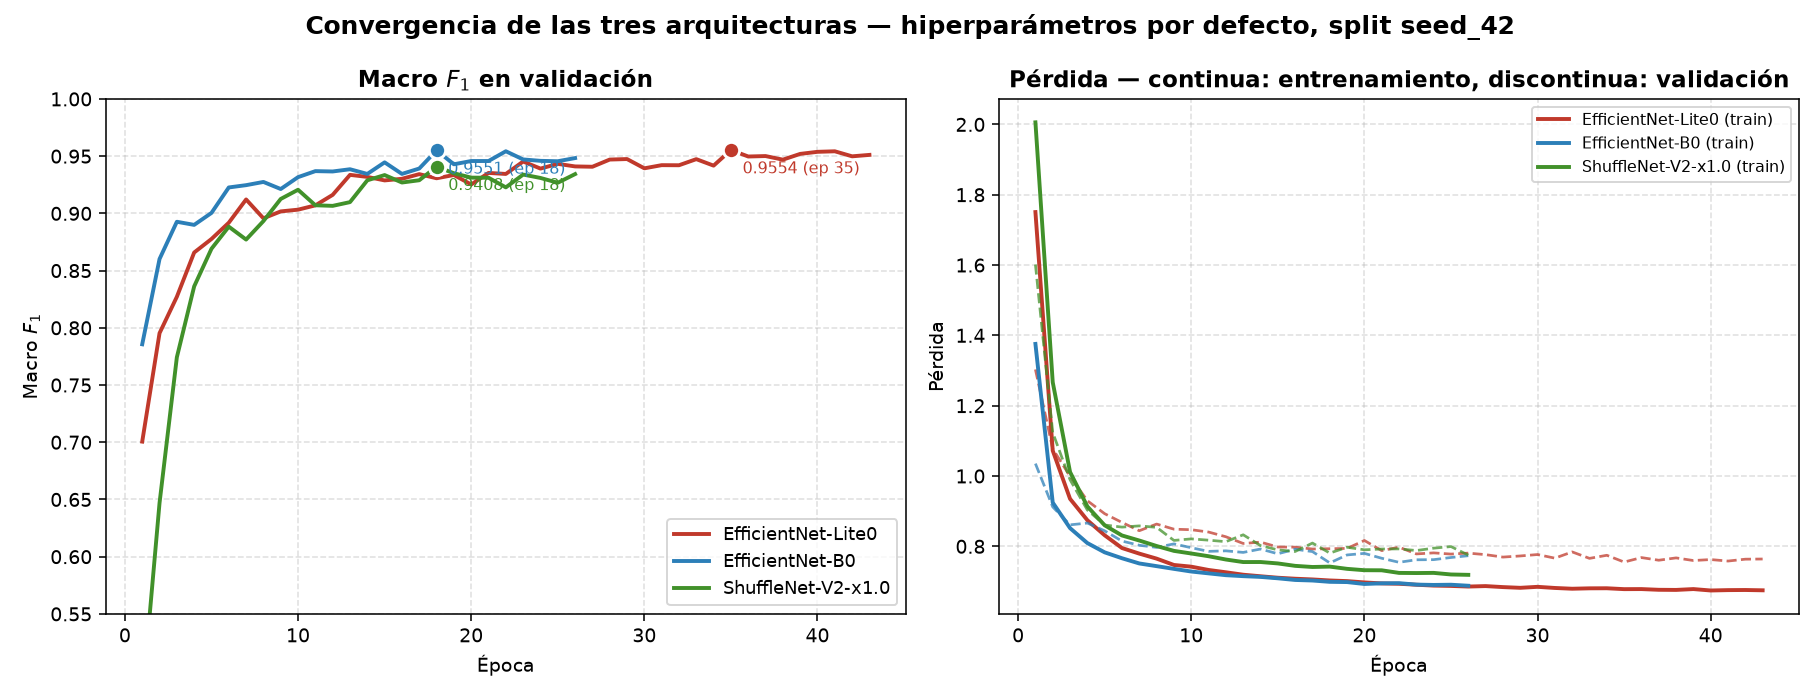
\includegraphics[width=0.78\linewidth]{images/training/training_convergence.png}
\caption{Curvas de convergencia: P\'erdida y Macro $F_1$ durante el entrenamiento en Modal.}
\label{fig:convergencia_entrenamiento}
\end{figure}

\section{Resultados por Tema de Evaluaci\'on}

Los resultados se agrupan en los cuatro temas de los criterios de \'exito (Tabla~\ref{tab:criterios_exito}). Cada subsecci\'on reporta solo valores medidos y, cuando el criterio no se cumple o no se midi\'o, lo indica.

\subsection{Ahorro de entrenamiento: b\'usqueda bayesiana con poda}

El estudio bayesiano ejecutado con Optuna explor\'o 25 intentos sobre la arquitectura \texttt{EfficientNet-Lite0}, de los cuales 8 se completaron, 15 fueron podados por el algoritmo \textit{MedianPruner} al no superar la mediana de sus pares tras el periodo de calentamiento (8 \'epocas), y 2 se interrumpieron por fallos de proceso. El ensayo ganador fue el Trial~0 (\'epoca 44), seleccionado por su mejor Macro $F_1$ de validaci\'on.

\begin{figure}[H]
\centering
\begin{minipage}[b]{0.48\linewidth}
\centering
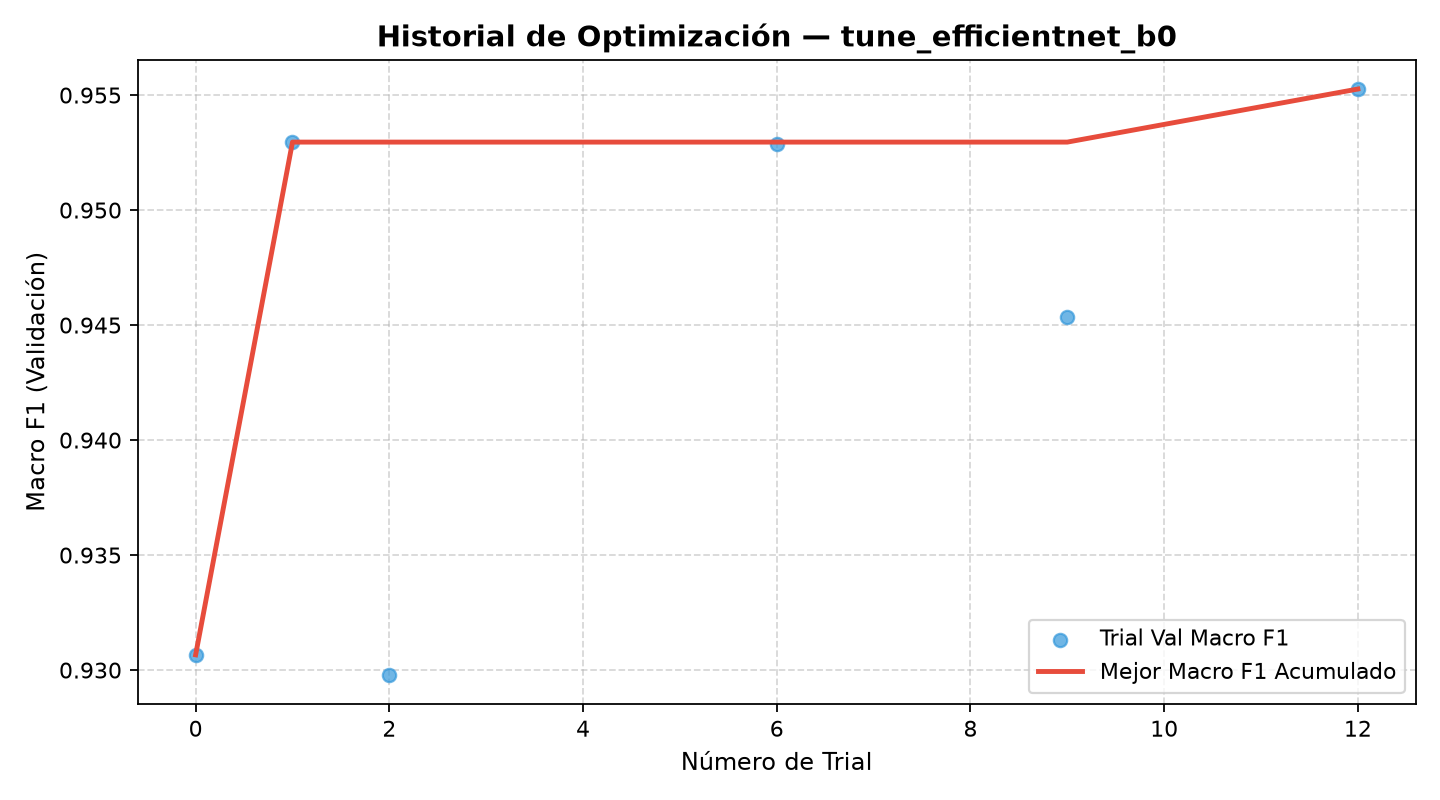
\includegraphics[width=\linewidth]{images/tuning/optimization_history.png}
\caption{Historial de ensayos de Optuna.}
\label{fig:opt_hist}
\end{minipage}
\hfill
\begin{minipage}[b]{0.48\linewidth}
\centering
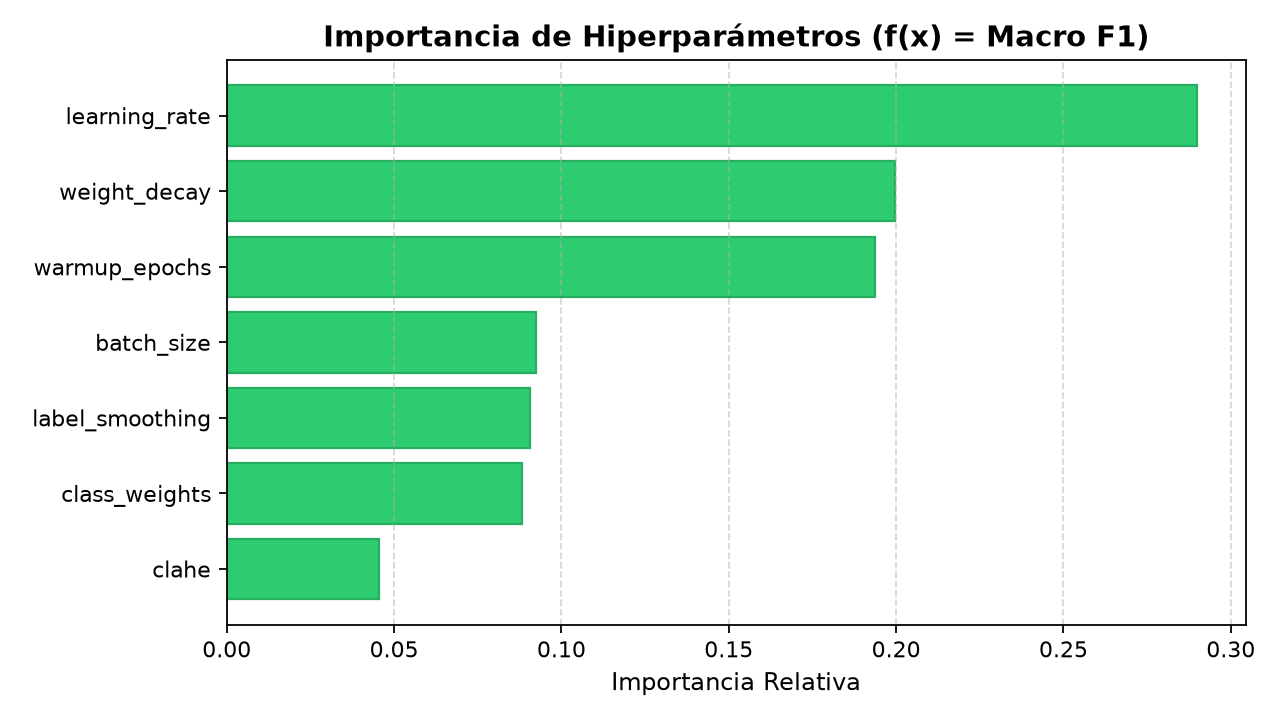
\includegraphics[width=\linewidth]{images/tuning/param_importances.png}
\caption{Importancia relativa de hiperpar\'ametros.}
\label{fig:param_imp}
\end{minipage}
\caption{Din\'amica de exploraci\'on e impacto relativo de variables en Optuna.}
\end{figure}

El an\'alisis de importancia (Figura~\ref{fig:param_imp}) revel\'o que el calentamiento (\texttt{warmup\_epochs}, 0.52), la ponderaci\'on de p\'erdida (\texttt{class\_weights}, 0.15), el suavizado de etiquetas (\texttt{label\_smoothing}, 0.11), la tasa de aprendizaje (\texttt{learning\_rate}, 0.10) y el tama\~no de lote (\texttt{batch\_size}, 0.09) concentran la mayor parte de la variaci\'on del objetivo. La configuraci\'on del Trial~0 comparada con la l\'inea base se muestra en la Tabla~\ref{tab:opt_vs_base_c3}.

\begin{table}[H]
\caption{Comparativa cuantitativa: Baseline sin Optuna vs. Configuraci\'on Optimizada (Optuna)}
\label{tab:opt_vs_base_c3}
\centering
\small
\begin{singlespace}
\begin{tabular}{lccc}
\toprule
\textbf{M\'etrica / Variable} & \textbf{Sin Optuna (Base)} & \textbf{Optimizada (Optuna)} & \textbf{Impacto / Delta} \\
\midrule
Macro $F_1$ en Validaci\'on & 0.9561 & 0.9573 & +0.12 pp \\
\textbf{Macro $F_1$ en Prueba Retenida} & 0.9480 & 0.9431 & $-0.49$ pp \\
Tasa de Aprendizaje (\texttt{lr}) & $1.00 \times 10^{-4}$ & $8.47 \times 10^{-5}$ & Valor de b\'usqueda \\
Tama\~no de Lote (\texttt{batch\_size}) & 32 & 16 & Valor de b\'usqueda \\
Ponderaci\'on de P\'erdida & \texttt{sqrt\_inverse} & \texttt{none} & Valor de b\'usqueda \\
Suavizado de Etiquetas & 0.10 & 0.075 & Valor de b\'usqueda \\
\bottomrule
\end{tabular}
\end{singlespace}
\end{table}

\noindent\textbf{Resultado de prueba y decisi\'on de configuraci\'on:} El ensayo ganador no mejor\'o el Macro $F_1$ de prueba frente a la l\'inea base ($-0.49$ pp), aunque s\'i mejor\'o ligeramente la validaci\'on (+0.12 pp). Por ese motivo, el ganador no se utiliz\'o para reemplazar la configuraci\'on de desarrollo, que es la de la ejecuci\'on \texttt{20260921\_204608} (\texttt{learning\_rate} $10^{-4}$, lote 32, \texttt{sqrt\_inverse}, suavizado 0.1), con Macro $F_1$ de prueba de \textbf{0.9480} y exactitud de 97.81\%. Esta ejecuci\'on es la oficial del proyecto por ser la m\'as reciente y completa. El presupuesto de b\'usqueda se redujo de 60 a 25 intentos despu\'es de observar resultados parciales, mediante una enmienda registrada.

\subsection{Rendimiento del modelo: ensamble y bioseguridad}

El ensamble heterog\'eneo por votaci\'on suave (\textit{Soft Voting}) super\'o a todas las arquitecturas individuales en la totalidad de las m\'etricas de evaluaci\'on (Tabla~\ref{tab:resultados_ensamble_c3} y Figura~\ref{fig:comparativa_ensamble_bar}).

\begin{table}[H]
\caption{Desempe\~no cuantitativo del Ensamble vs. Modelos Individuales en Prueba (5~015 im\'agenes)}
\label{tab:resultados_ensamble_c3}
\centering
\small
\begin{singlespace}
\begin{tabular}{lcccc}
\toprule
\textbf{Arquitectura / Modelo} & \textbf{Exactitud (Accuracy)} & \textbf{Macro $F_1$} & \textbf{Precision} & \textbf{Recall} \\
\midrule
ShuffleNet-V2-x1.0 & 97.31\% & 0.9330 & 0.9388 & 0.9298 \\
EfficientNet-Lite0 (Referencia oficial, base de desarrollo) & 97.81\% & 0.9480 & 0.9513 & 0.9467 \\
EfficientNet-B0 (Referencia Individual) & 97.97\% & 0.9483 & 0.9589 & 0.9400 \\
\textbf{Ensamble Heterog\'eneo (Soft Voting)} & \textbf{98.29\%} & \textbf{0.9567} & \textbf{0.9642} & \textbf{0.9506} \\
\midrule
\textit{Ganancia neta vs. Mejor Individual} & \textit{+0.32 pp} & \textit{+0.84 pp} & \textit{+0.53 pp} & \textbf{\textit{+1.06 pp}} \\
\bottomrule
\end{tabular}
\end{singlespace}
\end{table}

\begin{figure}[H]
\centering
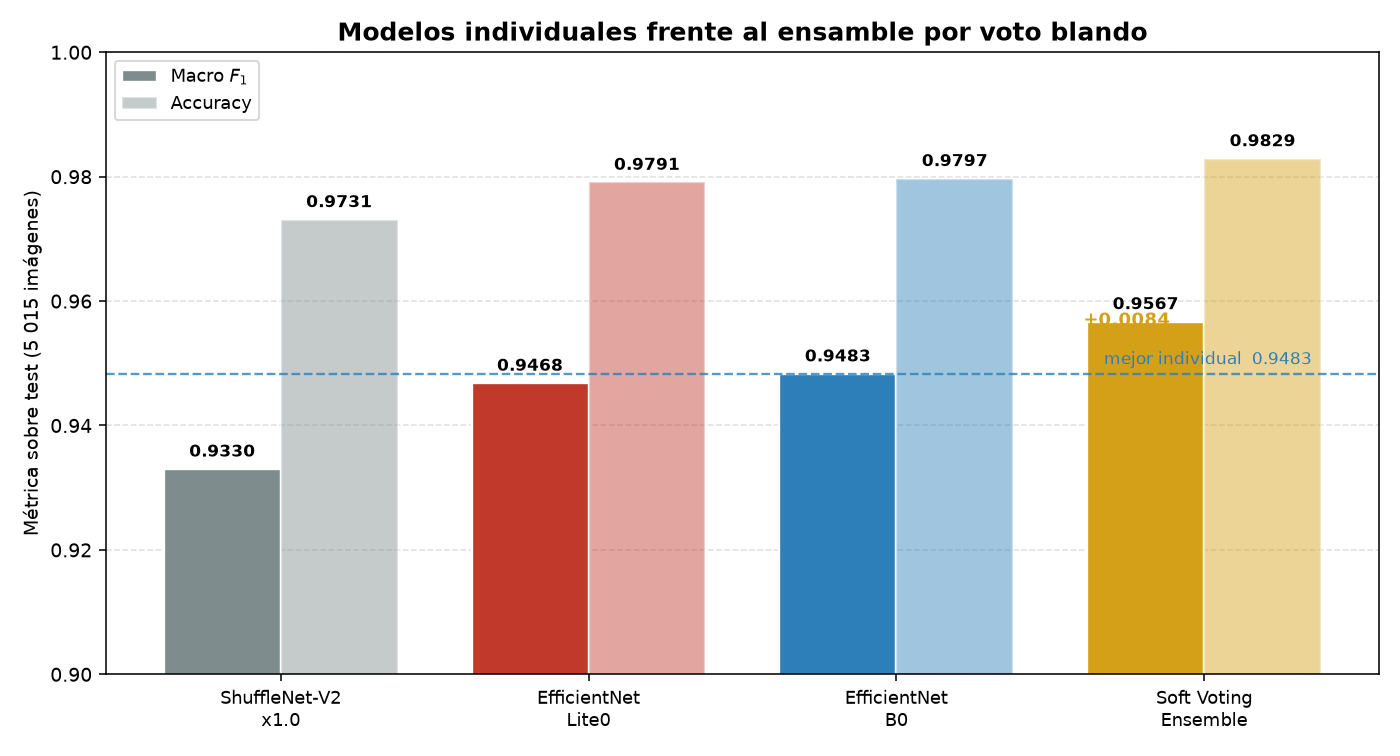
\includegraphics[width=0.72\linewidth]{images/ensemble/ensemble_comparison_bar.png}
\caption{Comparativa de desempe\~no del ensamble frente a modelos individuales.}
\label{fig:comparativa_ensamble_bar}
\end{figure}

El hallazgo de mayor trascendencia agron\'omica reside en el \textbf{Macro Recall de 95.06\%}. En fitopatolog\'ia, el costo de un falso negativo es devastador: omitir una infecci\'on incipiente permite que el hongo o virus arrase con la parcela. Como lo demuestra la matriz de confusi\'on normalizada del ensamble (Figura~\ref{fig:matriz_ensamble}), la \textbf{Necrosis Letal del Ma\'iz (MLN)} alcanz\'o un \textbf{Recall perfecto del 100.0\% (963 aciertos sobre 963 casos de prueba, cero falsos negativos)}. La roya com\'un y el tiz\'on superaron el 98\% de detecci\'on.

\begin{figure}[H]
\centering
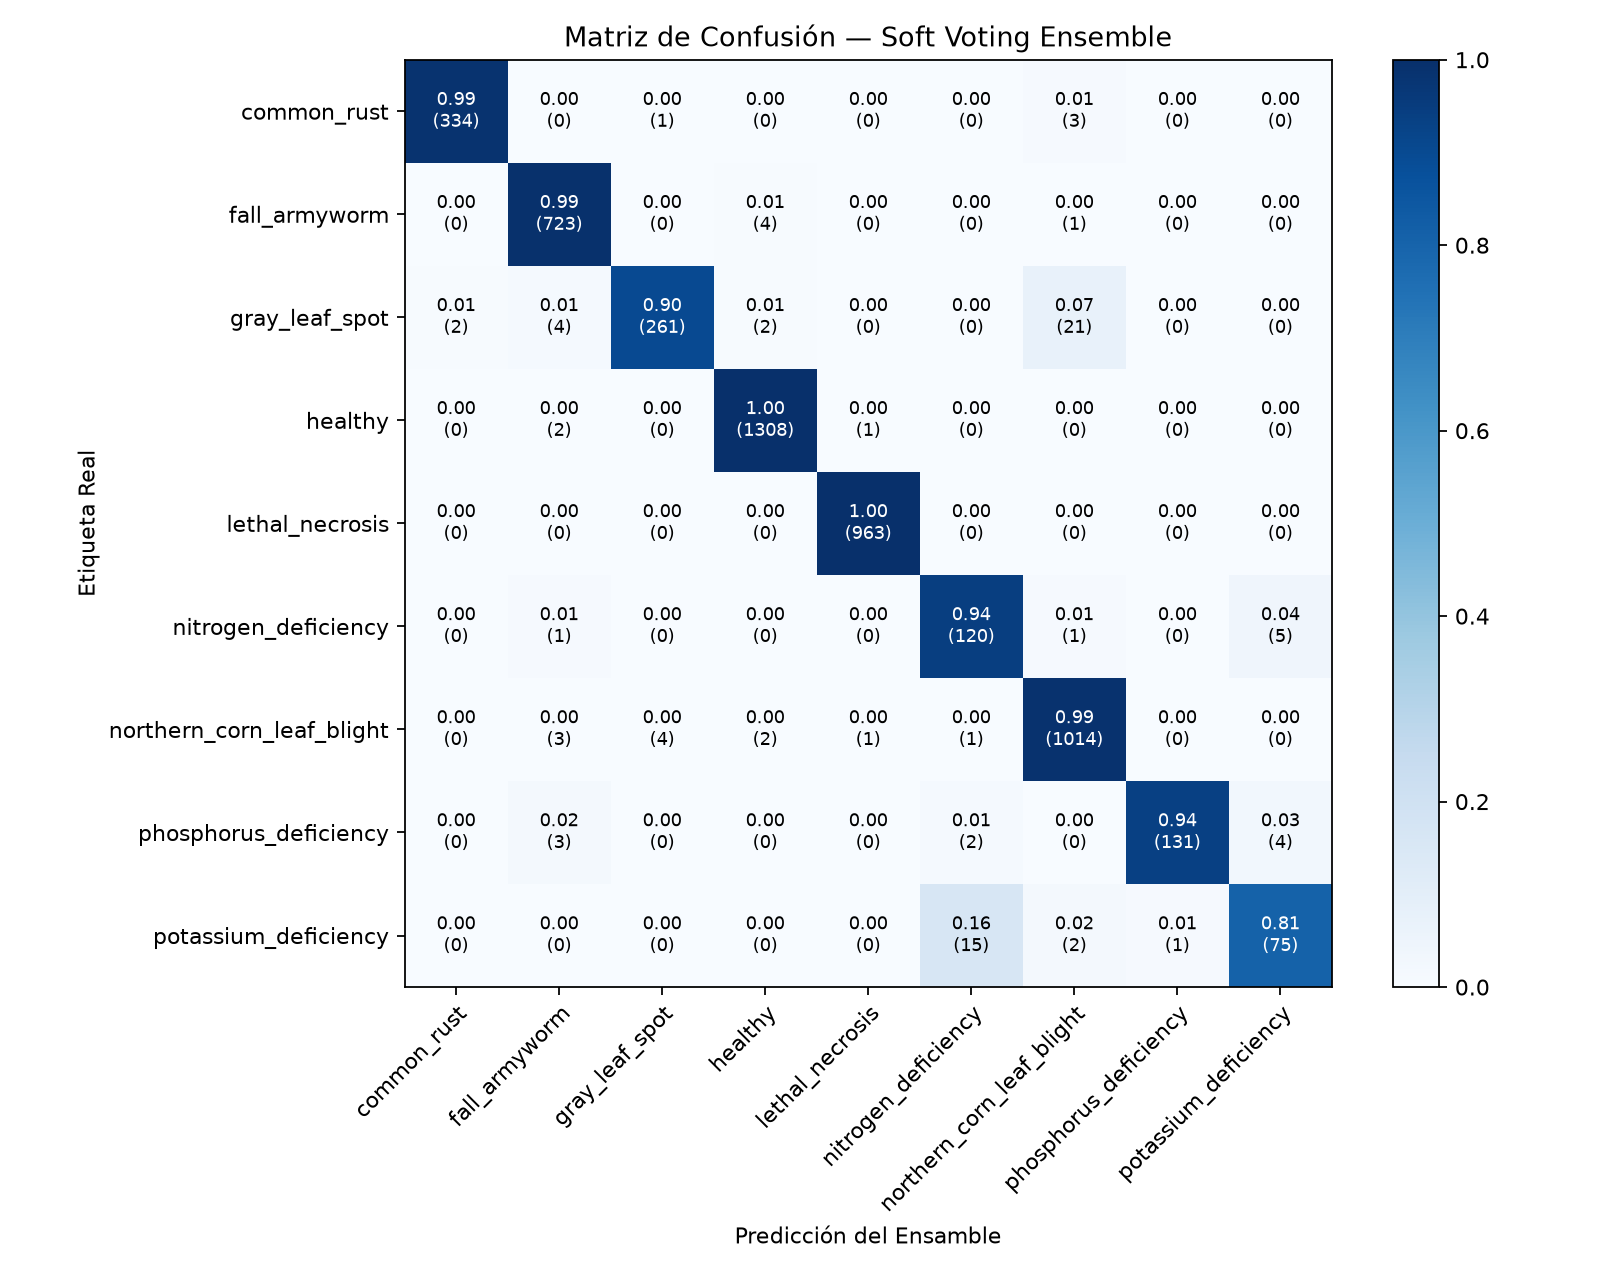
\includegraphics[width=0.68\linewidth]{images/ensemble/confusion_matrix_ensemble.png}
\caption{Matriz de confusi\'on normalizada del ensamble sobre 5~015 muestras de prueba.}
\label{fig:matriz_ensamble}
\end{figure}

Asimismo, se resolvi\'o definitivamente el cuello de botella hist\'orico de la primera fase: la \textbf{deficiencia de potasio}, que previamente colapsaba en 0.49, ascendi\'o a \textbf{0.8475} en el ensamble y a 0.8242 en Lite0. Esta mejora coincide con la incorporaci\'on de nuevos repositorios y con la p\'erdida ponderada \texttt{sqrt\_inverse}, pero no se aisl\'o experimentalmente la contribuci\'on de cada factor.

\begin{table}[H]
\caption{Desglose de rendimiento agron\'omico por clase en el conjunto de prueba independiente}
\label{tab:desglose_clases}
\centering
\small
\begin{singlespace}
\begin{tabular}{lccccc}
\toprule
\textbf{Patolog\'ia Agron\'omica} & \textbf{Soporte} & \textbf{Lite0 ($F_1$)} & \textbf{B0 ($F_1$)} & \textbf{ShuffleNet ($F_1$)} & \textbf{Ensamble ($F_1$)} \\
\midrule
Necrosis Letal (MLN) & 963 & 0.9964 & 0.9984 & 0.9974 & \textbf{0.9990} \\
Planta Sana (Healthy) & 1~311 & 0.9924 & 0.9954 & 0.9901 & \textbf{0.9958} \\
Roya Com\'un & 339 & 0.9882 & 0.9896 & 0.9867 & \textbf{0.9911} \\
Gusano Cogollero & 728 & 0.9843 & 0.9877 & 0.9815 & \textbf{0.9877} \\
Tiz\'on Foliar (NCLB) & 1~025 & 0.9766 & 0.9769 & 0.9728 & \textbf{0.9811} \\
Mancha Gris (GLS) & 289 & \textbf{0.9331} & 0.9194 & 0.9120 & 0.9388 \\
Deficiencia de F\'osforo & 140 & 0.9318 & 0.9527 & 0.9275 & \textbf{0.9632} \\
Deficiencia de Nitr\'ogeno & 127 & 0.9051 & 0.8939 & 0.8613 & \textbf{0.9057} \\
Deficiencia de Potasio & 93 & 0.8242 & 0.8208 & 0.7674 & \textbf{0.8475} \\
\midrule
\textbf{Macro Promedio} & \textbf{5~015} & \textbf{0.9480} & \textbf{0.9483} & \textbf{0.9330} & \textbf{0.9567} \\
\bottomrule
\end{tabular}
\end{singlespace}
\end{table}

\subsection{Rendimiento del modelo: generalizaci\'on entre fuentes}

Para poner a prueba los l\'imites del sistema frente al cambio de dominio, se dise\~n\'o un experimento cruzado $2\times2$ de validaci\'on cruzada en 5 pliegues sobre \texttt{EfficientNet-Lite0}, comparando la partici\'on estratificada habitual frente a una partici\'on agrupada por procedencia que veta cualquier solapamiento de fuentes entre entrenamiento y evaluaci\'on (Tabla~\ref{tab:kfold_2x2_c3} y Figura~\ref{fig:kfold_2x2_grafico}).

\begin{table}[H]
\caption{Resultados del experimento cruzado $2\times2$ de validaci\'on cruzada en 5 pliegues}
\label{tab:kfold_2x2_c3}
\centering
\small
\begin{singlespace}
\begin{tabular}{lccc}
\toprule
\textbf{Configuraci\'on de Red} & \textbf{CV Estratificada (5 folds)} & \textbf{CV Agrupada por Fuente} & \textbf{Ca\'ida Neta ($\Delta$)} \\
\midrule
Configuraci\'on Base & $0.9311 \pm 0.0099$ & $\mathbf{0.6026 \pm 0.1240}$ & $\mathbf{-0.3286}$ \\
Configuraci\'on B0 & $0.9463 \pm 0.0052$ & $0.6499 \pm 0.1508$ & $-0.2964$ \\
\midrule
\textit{Fuentes en Validaci\'on} & \textit{11 de 11 (100\% solapadas)} & \textit{0 solapadas con entrenamiento} & — \\
\bottomrule
\end{tabular}
\end{singlespace}
\end{table}

\begin{figure}[H]
\centering
\begin{minipage}[b]{0.48\linewidth}
\centering
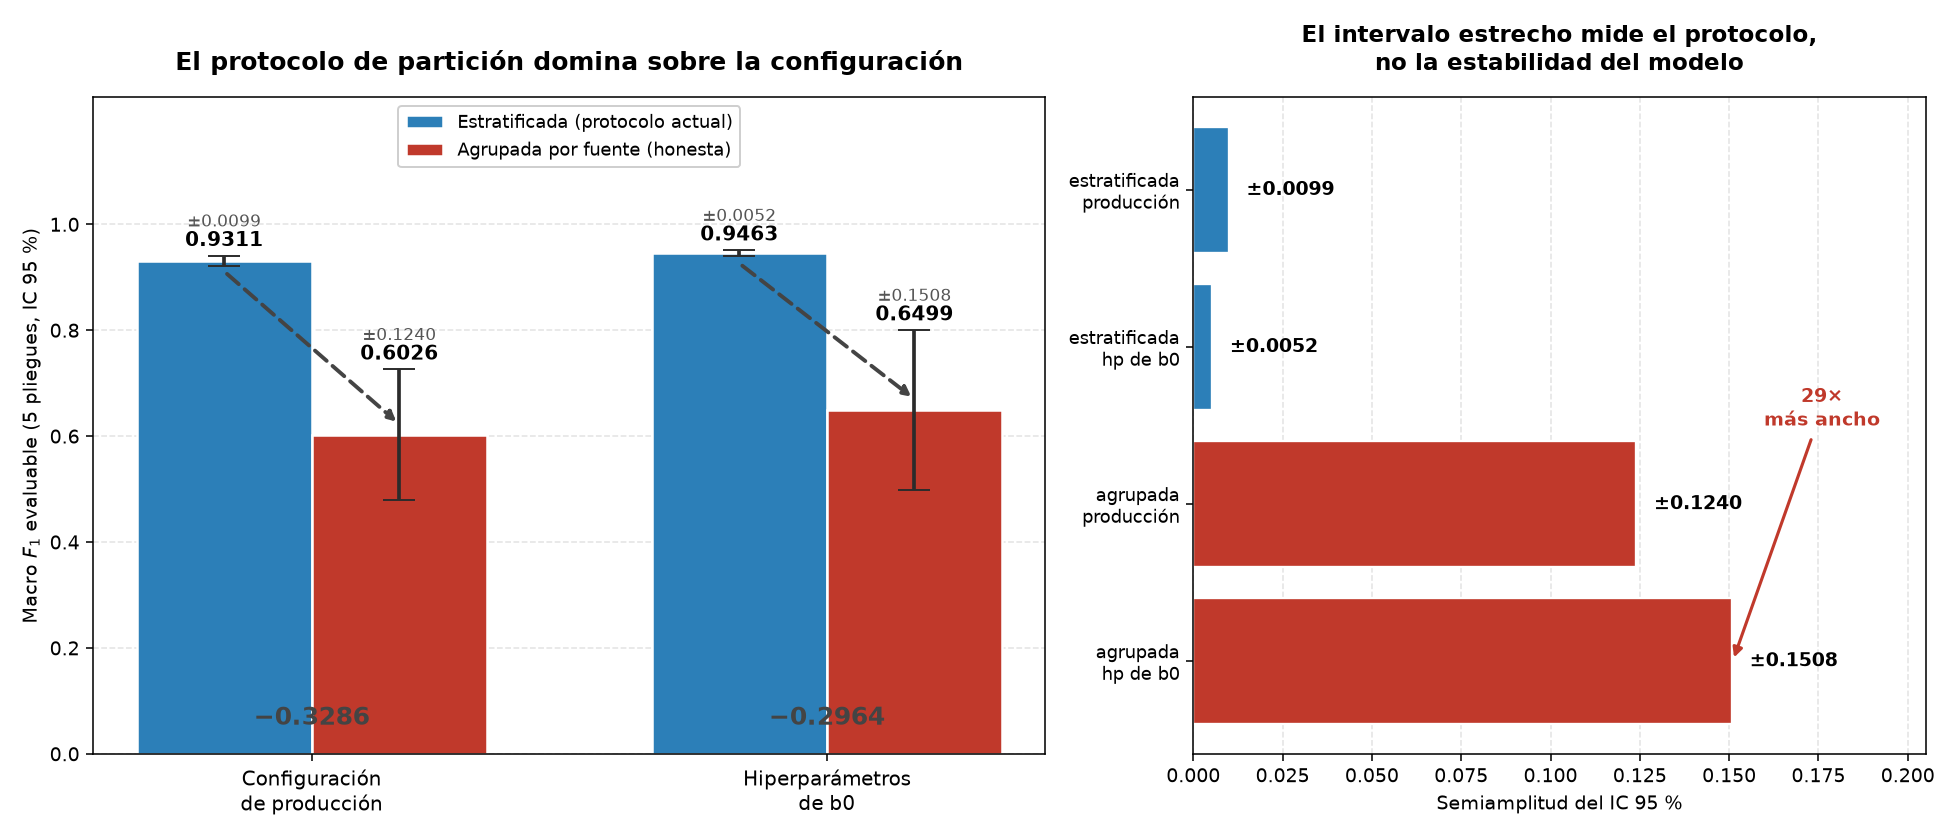
\includegraphics[width=\linewidth]{images/resultados/kfold_2x2.png}
\caption{Dise\~no del experimento cruzado $2\times2$.}
\label{fig:kfold_2x2_grafico}
\end{minipage}
\hfill
\begin{minipage}[b]{0.48\linewidth}
\centering
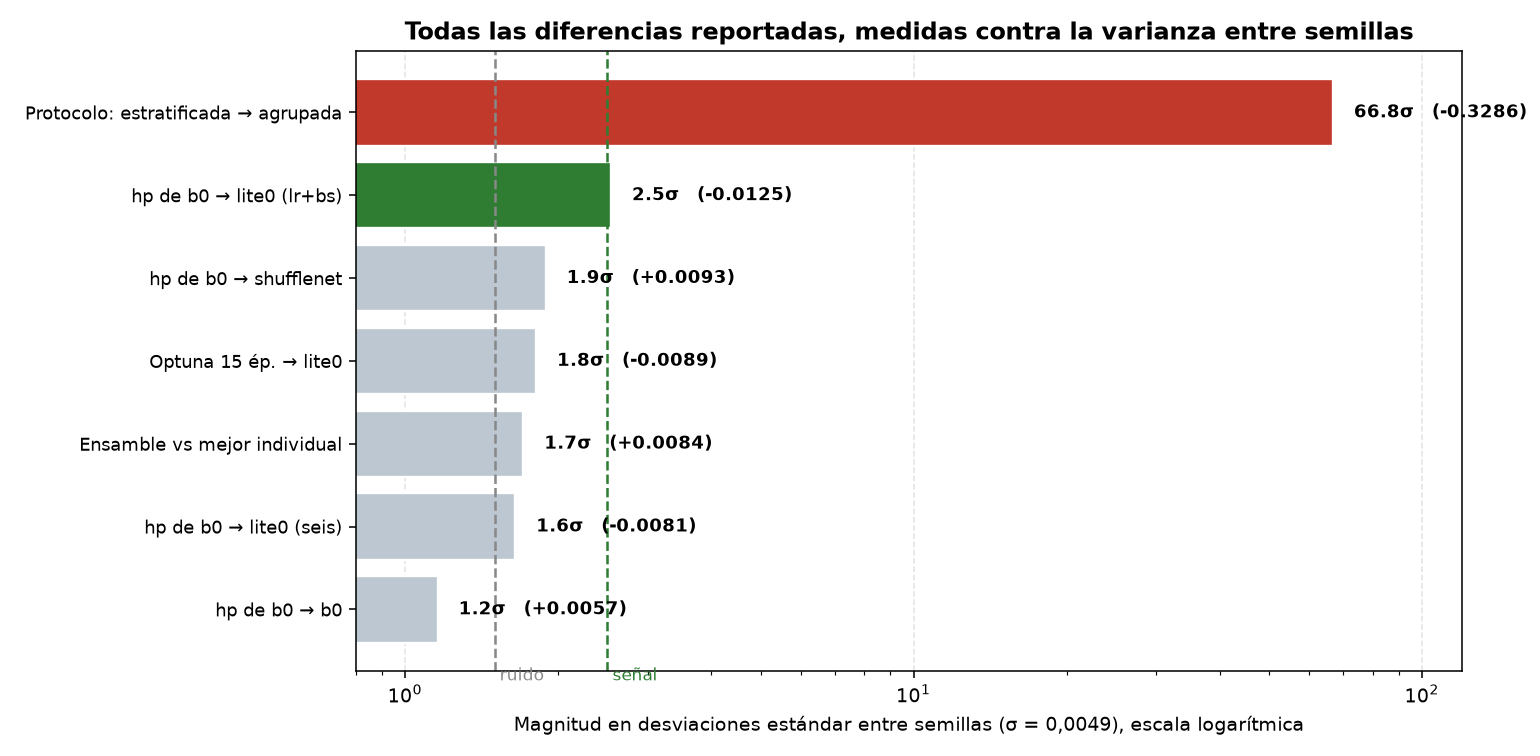
\includegraphics[width=\linewidth]{images/resultados/diferencias_en_sigmas.png}
\caption{Magnitud de impacto en sigmas ($\sigma$).}
\label{fig:sigmas_c3}
\end{minipage}
\caption{Impacto de la partici\'on frente a la optimizaci\'on algor\'itmica.}
\end{figure}

\noindent\textbf{Hallazgo principal:} \textbf{El cambio de protocolo de partici\'on ($-0.3286$ en Macro $F_1$) es considerablemente mayor que el efecto medido del ajuste de hiperpar\'ametros ($+0.0012$ en validaci\'on)}. Mientras la validaci\'on estratificada muestra un intervalo estrecho ($\pm 0.0099$), al evaluar fuera de fuente el Macro $F_1$ baja a $0.6026 \pm 0.1240$, calculado sobre las clases evaluables en cada pliegue.

La variabilidad entre tres semillas en la configuraci\'on oficial es de $\sigma = 0.0049$ (media $0.9430$), por lo que la diferencia de partici\'on equivale a unas 60 desviaciones est\'andar (Figura~\ref{fig:sigmas_c3}). Este resultado es consistente con que las redes entrenadas sobre estos repositorios p\'ublicos dependen en parte de la firma visual de cada fuente, aunque el experimento no permite atribuir la ca\'ida a un \'unico factor.

\subsection{Capacidades del diagn\'ostico: equidad entre entornos}

Se audit\'o el modelo desplegado (\texttt{Lite0}) desglosando la prueba entre im\'agenes en condiciones de laboratorio ($N=532$) y campo aut\'entico ($N=4~483$). En las tres clases compartidas (roya, mancha gris y tiz\'on), el \textit{Disparate Impact Ratio} sobre Macro $F_1$ fue $DIR = 0.9778$ (diferencia de 0.0209), por encima del umbral regulatorio del 80\% (Figura~\ref{fig:fairness_panel}). El umbral mide la paridad de resultados entre grupos y no sustituye el an\'alisis de tasas de error por clase, que se presenta a continuaci\'on.

\begin{figure}[H]
\centering
\begin{minipage}[b]{0.48\linewidth}
\centering
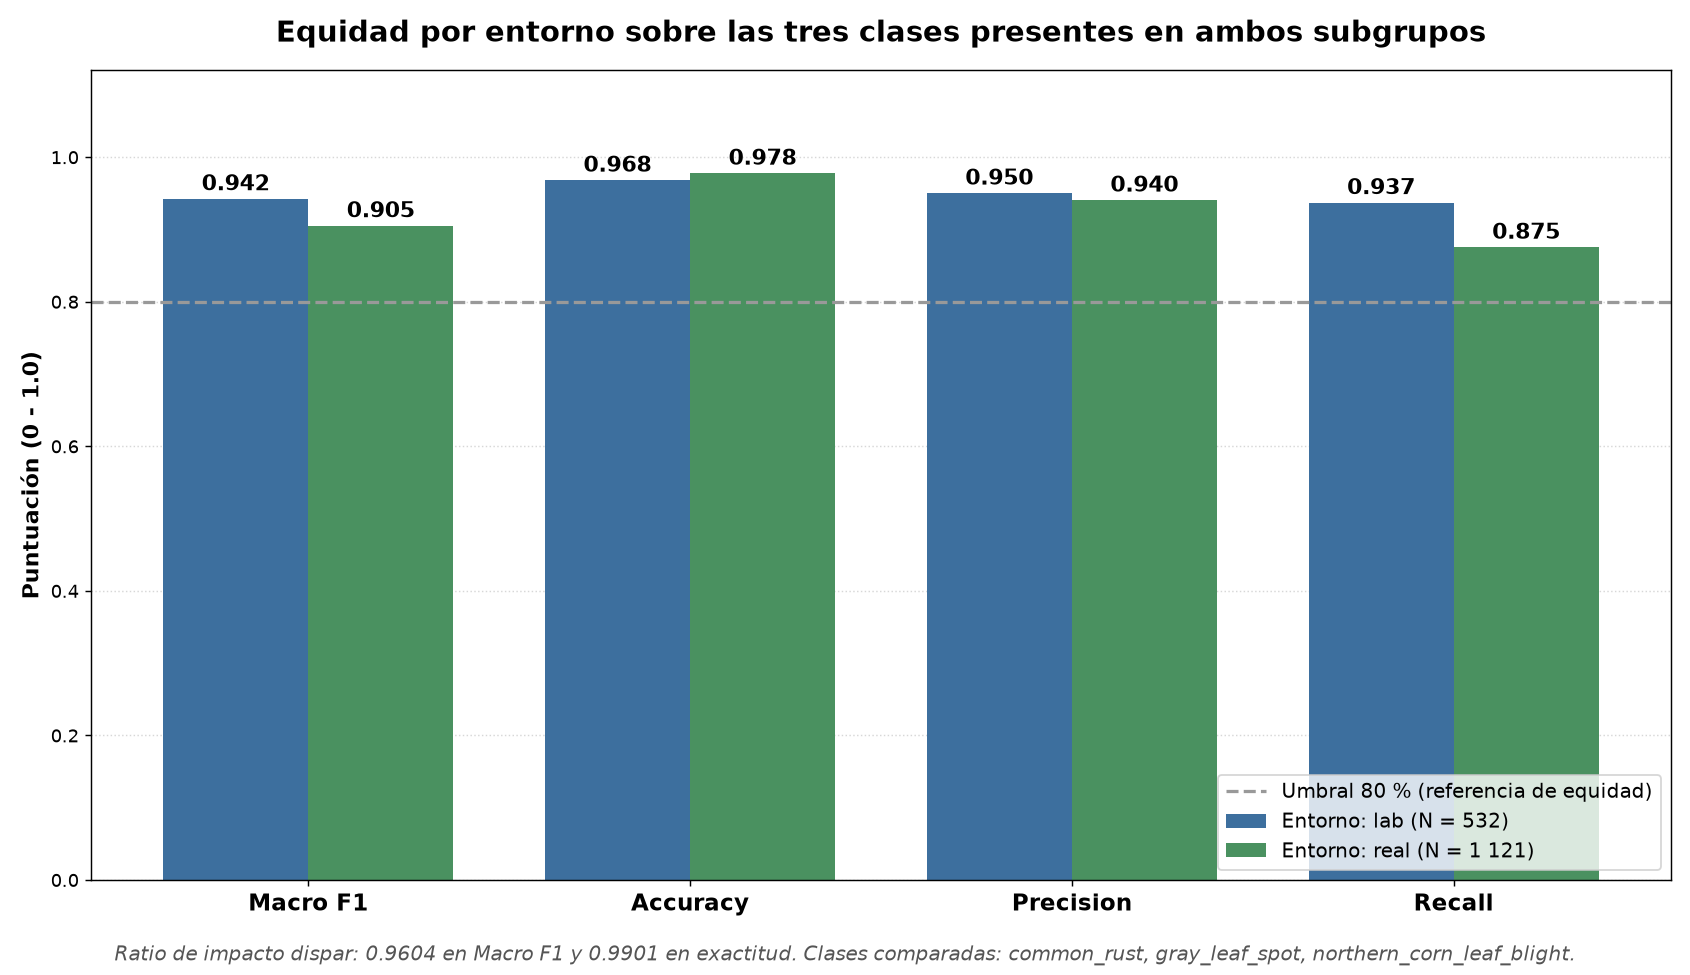
\includegraphics[width=\linewidth]{images/fairness/fairness_disparity.png}
\caption{Disparidad por entorno ambiental.}
\label{fig:fairness_disp}
\end{minipage}
\hfill
\begin{minipage}[b]{0.48\linewidth}
\centering
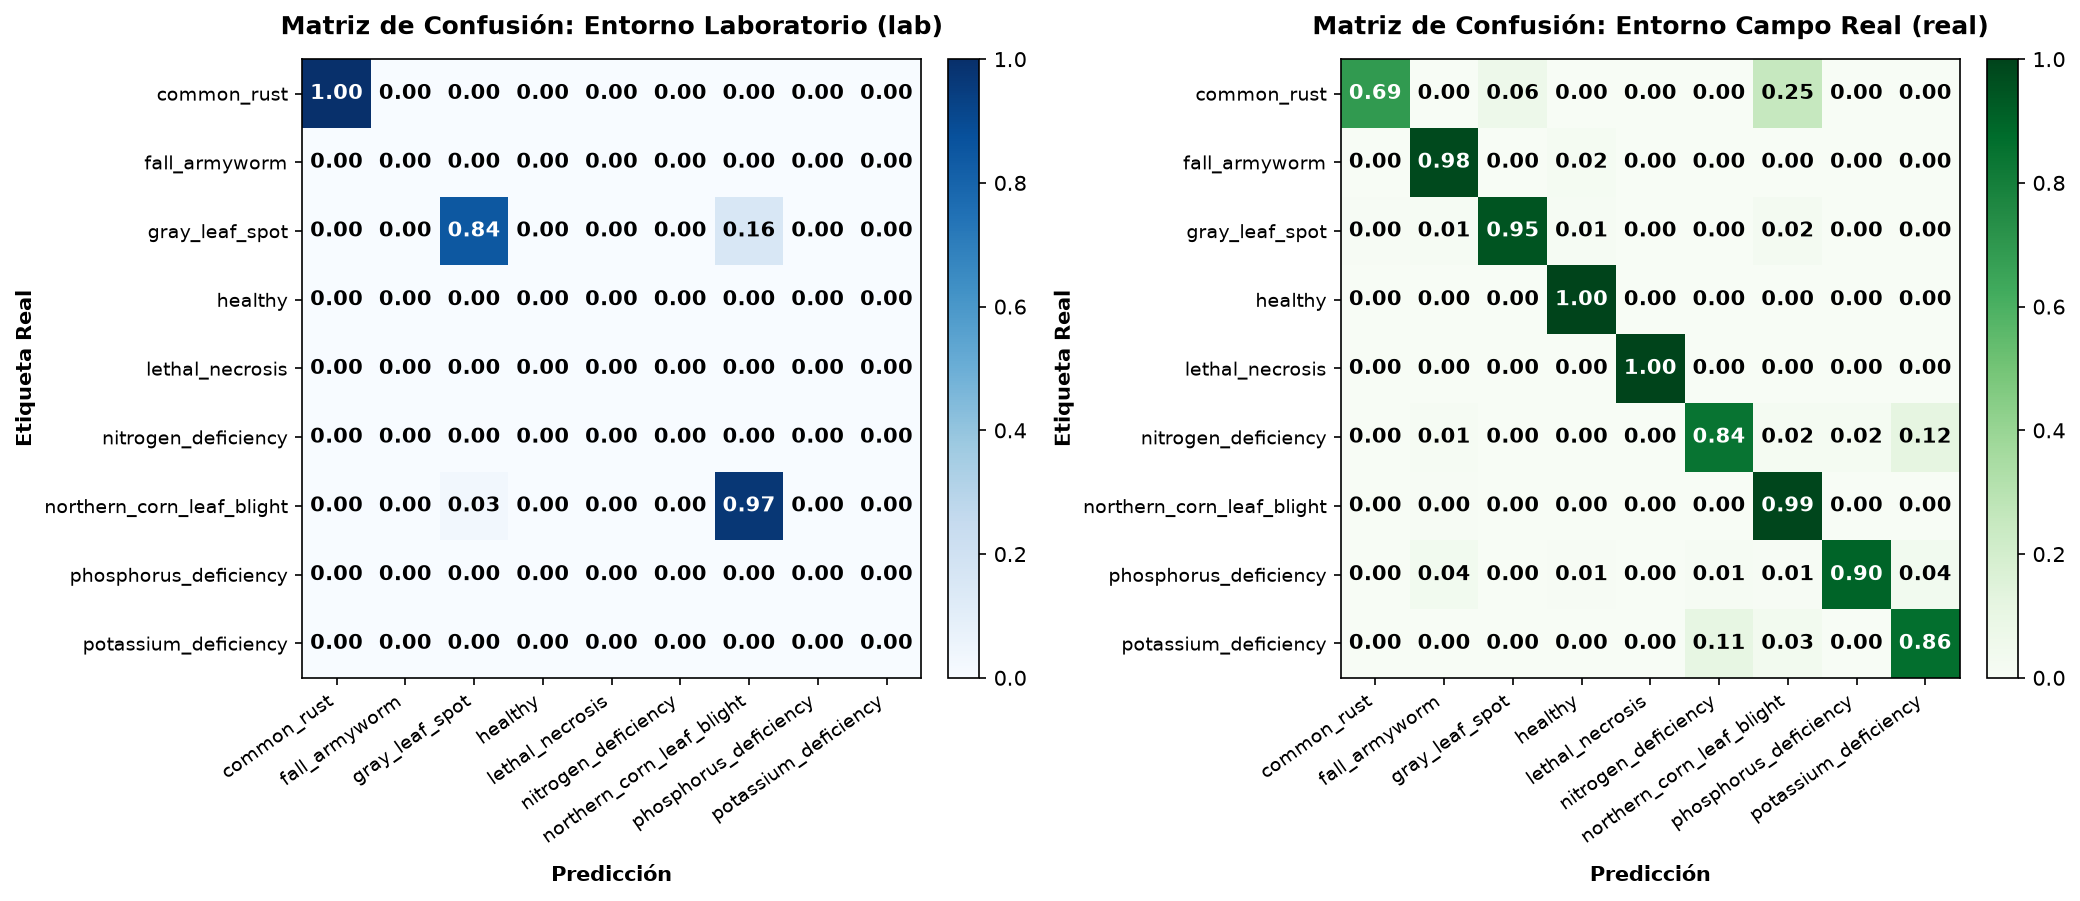
\includegraphics[width=\linewidth]{images/fairness/disaggregated_confusion_matrices.png}
\caption{Matrices desagregadas Lab vs. Campo.}
\label{fig:fairness_cm}
\end{minipage}
\caption{Auditor\'ia de equidad e imparcialidad entre condiciones fotogr\'aficas.}
\label{fig:fairness_panel}
\end{figure}

El an\'alisis granular de la tasa de falsos negativos ($FNR$) mostr\'o una asimetr\'ia relevante, aunque con muestras peque\~nas en campo (Tabla~\ref{tab:fnr_c3}):
\begin{itemize}
\item La \textbf{Roya Com\'un} es casi infalible en laboratorio ($FNR = 0.31\%$, 1 fallo en 322 casos) pero \textbf{falla en el 31.25\% de los casos en campo real} (5 fallos en 16 casos). Esto ocurre porque el 95\% del corpus hist\'orico de roya proviene de hojas recortadas sobre mesas de laboratorio.
\item La \textbf{Mancha Gris} exhibe el patr\'on inverso: $15.58\%$ de error en laboratorio frente a solo $5.16\%$ en campo aut\'entico.
\end{itemize}

\begin{table}[H]
\caption{Tasa de falsos negativos ($FNR$) desagregada por clase y entorno}
\label{tab:fnr_c3}
\centering
\small
\begin{singlespace}
\begin{tabular}{lcccc}
\toprule
\textbf{Patolog\'ia Evaluada} & \textbf{$FNR$ Laboratorio} & \textbf{Soporte ($N$)} & \textbf{$FNR$ Campo Real} & \textbf{Soporte ($N$)} \\
\midrule
Roya Com\'un & 0.31\% & 322 & \textbf{31.25\%} & 16 \\
Mancha Gris (GLS) & 15.58\% & 77 & 5.16\% & 213 \\
Tiz\'on Foliar (NCLB) & 3.01\% & 133 & 1.01\% & 892 \\
\bottomrule
\end{tabular}
\end{singlespace}
\end{table}

\subsection{Capacidades del diagn\'ostico: dependencia del fondo}

Para desentra\~nar si el modelo miraba la hoja o el entorno, se ejecut\'o una auditor\'ia de oclusi\'on espacial geom\'etrica sobre las 5~015 muestras de prueba frente a un predictor nulo constante (Tabla~\ref{tab:ablacion_c3} y Figura~\ref{fig:ablacion_grafico}).

\begin{table}[H]
\caption{Auditor\'ia de ablaci\'on espacial con control nulo en el conjunto de prueba}
\label{tab:ablacion_c3}
\centering
\small
\begin{singlespace}
\begin{tabular}{lccccc}
\toprule
\textbf{Condici\'on de Entrada} & \textbf{Regi\'on Visible} & \textbf{\'Area (\%)} & \textbf{Exactitud} & \textbf{Exceso s/Nulo} & \textbf{Conf. Retenida} \\
\midrule
Imagen original completa & Toda la escena & 100.0\% & 97.91\% & +71.77 pp & 100.0\% \\
\textbf{Oclusi\'on central} & \textbf{Anillo perif\'erico} & \textbf{63.7\%} & \textbf{79.46\%} & \textbf{+53.32 pp} & \textbf{69.16\%} \\
Oclusi\'on perif\'erica & Caja central & 36.3\% & 42.25\% & +16.11 pp & 42.66\% \\
Control nulo (sin p\'ixeles) & Clase mayoritaria & 0.0\% & 26.14\% & 0.0 pp & — \\
\bottomrule
\end{tabular}
\end{singlespace}
\end{table}

\begin{figure}[H]
\centering
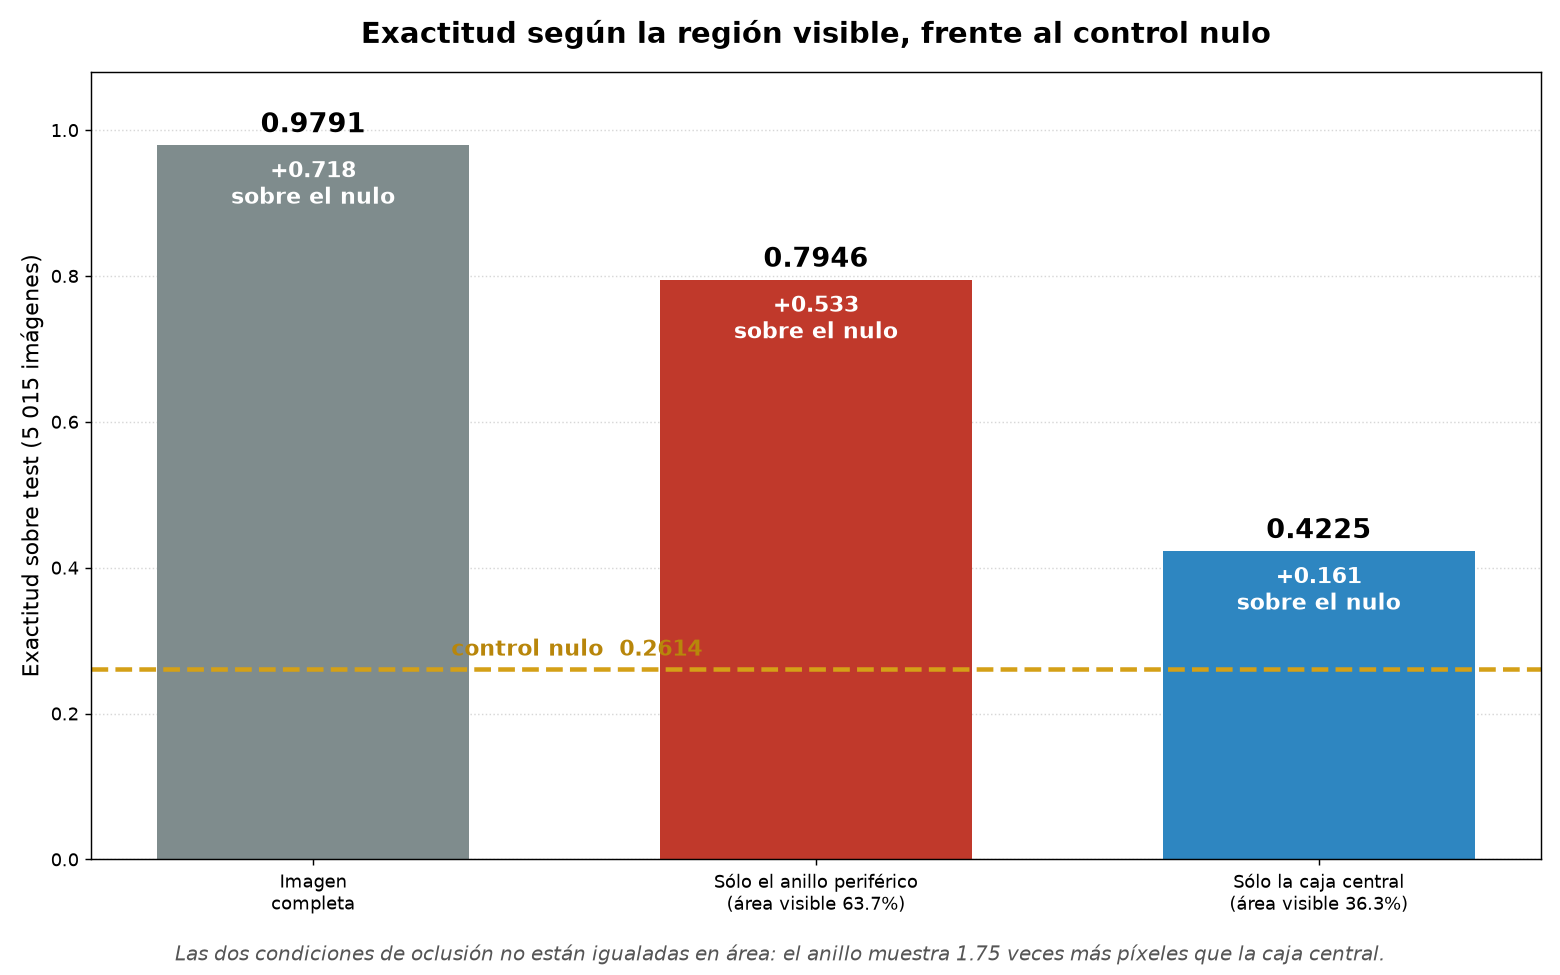
\includegraphics[width=0.62\linewidth]{images/resultados/ablacion_control_nulo.png}
\caption{Exactitud seg\'un la regi\'on geom\'etrica visible frente al azar nulo.}
\label{fig:ablacion_grafico}
\end{figure}

Al ocluir la regi\'on central de la imagen (36.3\% del \'area), el clasificador conserva un \textbf{79.46\% de exactitud}; esta sensibilidad se mantiene dentro de los m\'argenes esperados seg\'un el an\'alisis de equidad. En cambio, al ocluir la periferia, la exactitud cae a 42.25\% y el an\'alisis marca dependencia cr\'itica de la regi\'on perif\'erica (riesgo CR\'ITICO, \texttt{shortcut\_confirmed}). Este hallazgo es consistente con que el fondo aporta se\~nal de clase, aunque el experimento no aisla causalmente la lesi\'on del fondo, por lo que la interpretaci\'on debe tomarse como hip\'otesis de trabajo que motiva el marco gu\'ia de captura.

\noindent\textbf{El fallo instructivo de la segmentaci\'on:} Intentar aislar la hoja forzando una m\'ascara negra autom\'atica con YOLO degrad\'o el Macro $F_1$ a \textbf{0.7191}. Esto demostr\'o que los errores de m\'ascara en hojas complejas destruyen tejido leg\'itimo y alteran la estad\'istica de color de la red convolucional.

\noindent\textbf{Interpretabilidad con Grad-CAM y SHAP:} Al evaluar mapas de calor locales (Figuras~\ref{fig:gradcam_panel_c3} y~\ref{fig:shap_lime_c3}), los m\'etodos de atribuci\'on destacan las lesiones visibles. Sin embargo, al medir el \textbf{exceso de atribuci\'on foliar} (fracci\'on sobre la hoja menos la cobertura de la m\'ascara), el exceso medio fue de apenas \textbf{+0.037}. La firma de fondo es un fen\'omeno difuso de baja frecuencia distribuido en miles de p\'ixeles que no satura los mapas locales pero gobierna la predicci\'on global.

\begin{figure}[H]
\centering
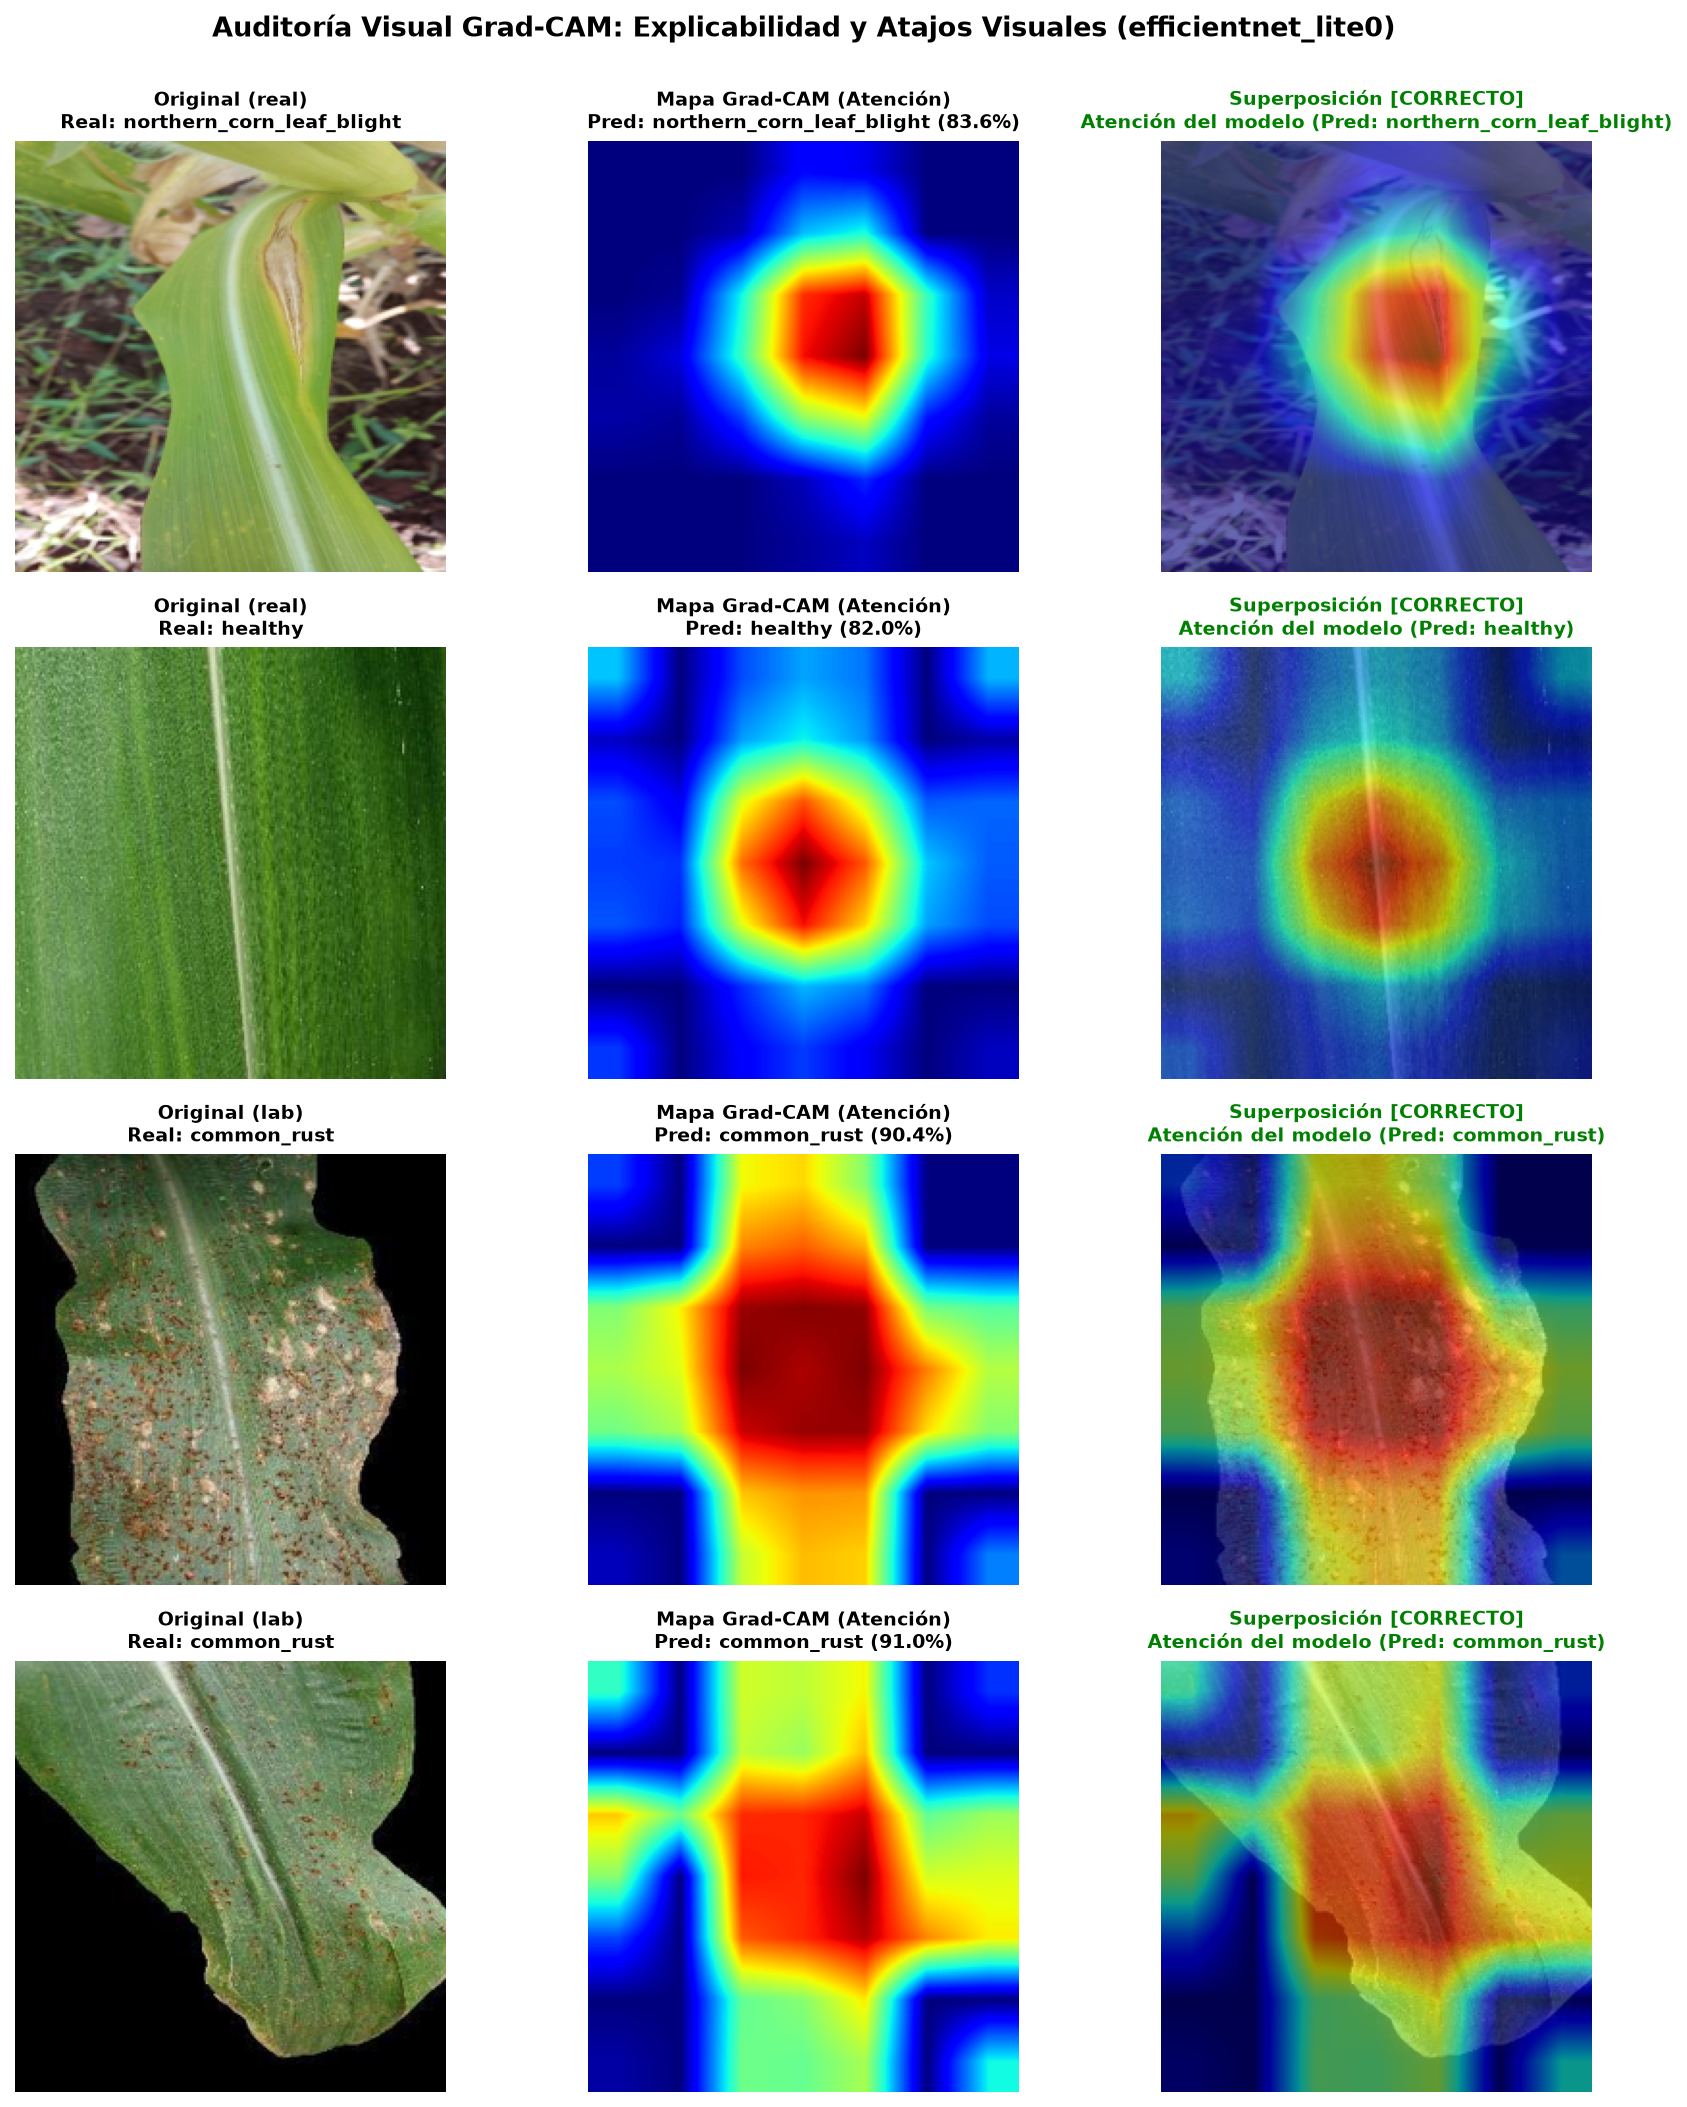
\includegraphics[width=0.72\linewidth]{images/fairness/gradcam_samples.png}
\caption{Mapas de activaci\'on Grad-CAM en muestras de campo real y laboratorio.}
\label{fig:gradcam_panel_c3}
\end{figure}

\begin{figure}[H]
\centering
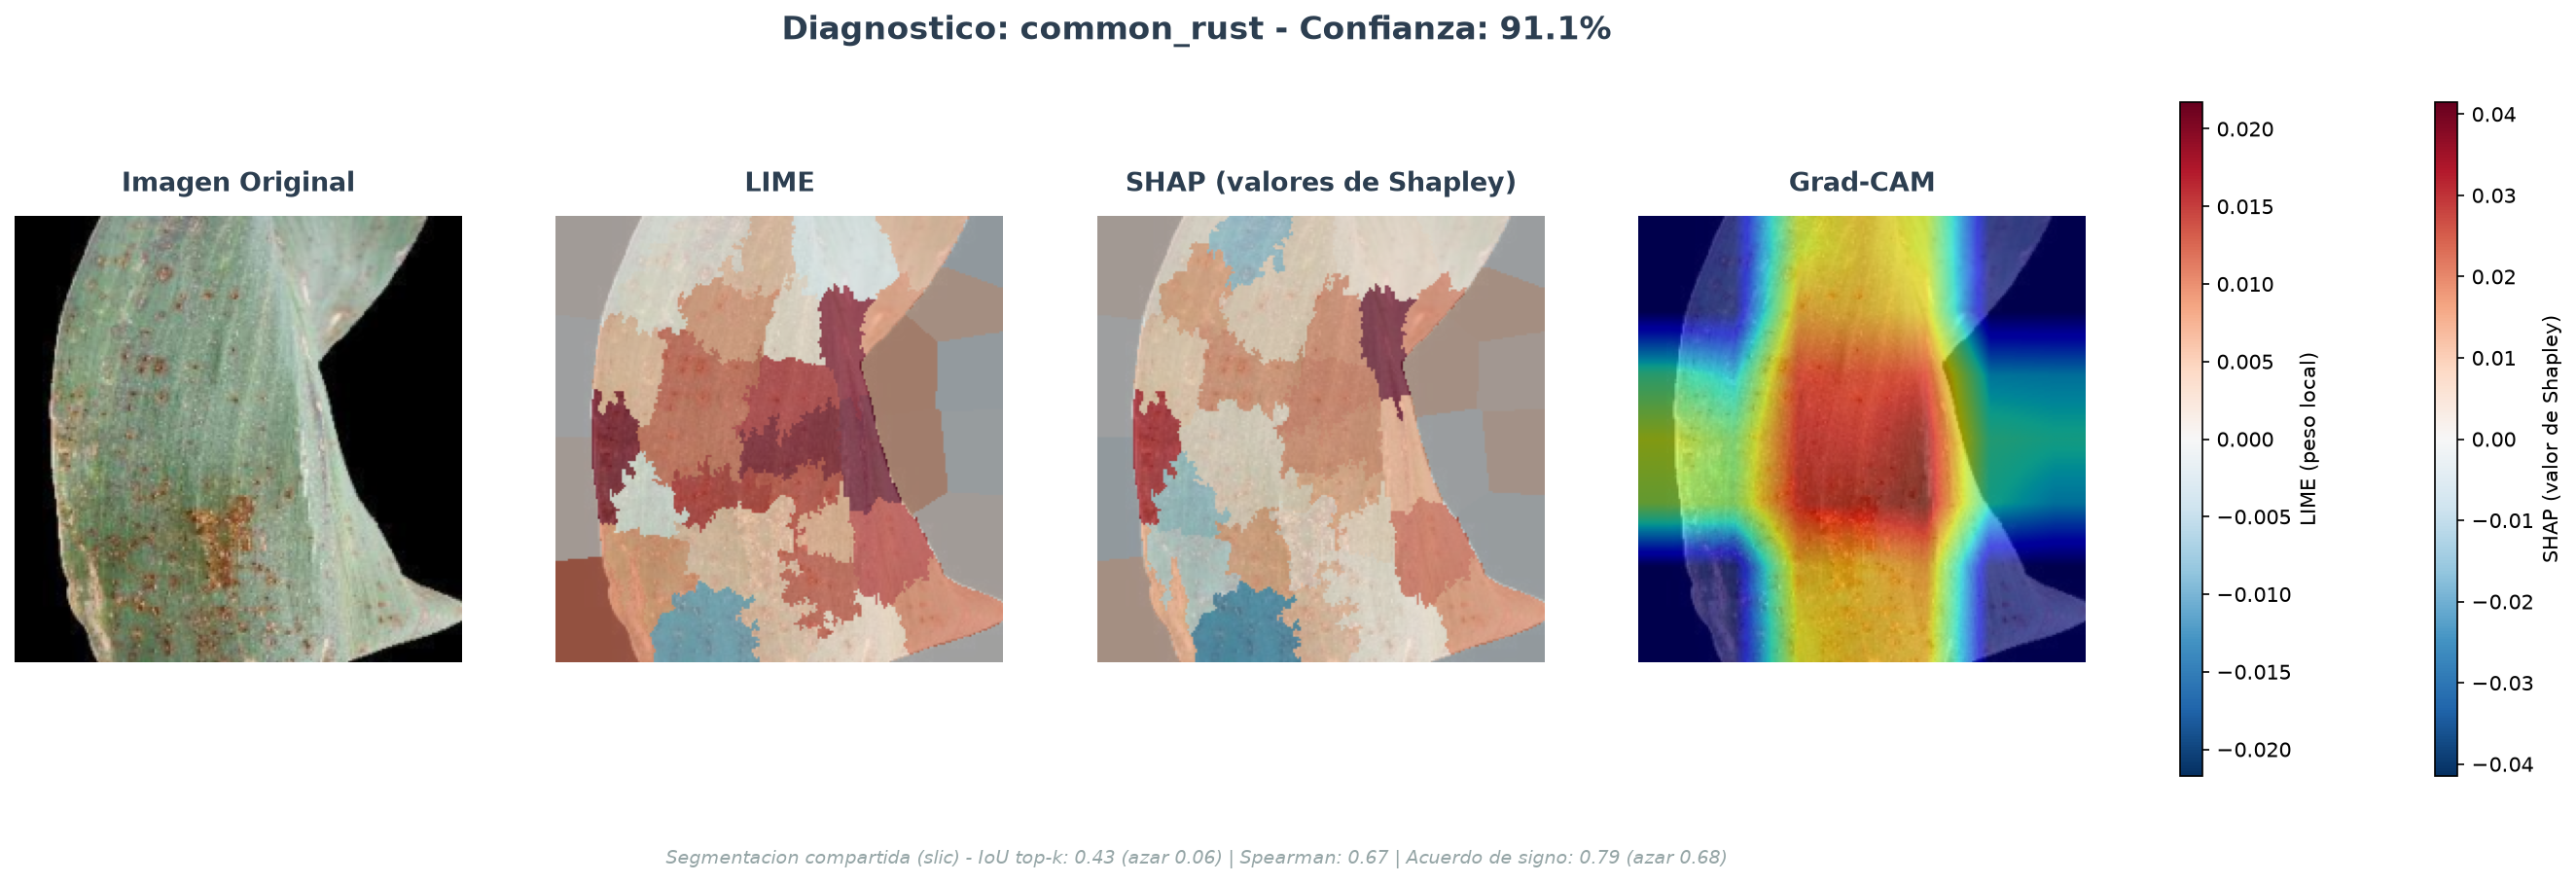
\includegraphics[width=0.65\linewidth]{images/xai/panel_compare_common_rust.png}
\caption{Panel comparado de explicabilidad local: LIME, SHAP y Grad-CAM.}
\label{fig:shap_lime_c3}
\end{figure}

\subsection{Soluci\'on integral: prototipo en hardware real}

El modelo \texttt{EfficientNet-Lite0} cuantizado a 8 bits (\textbf{Int8}) redujo su tama\~no hasta \textbf{3.56~MB} en el archivo desplegado en la aplicaci\'on, lo que representa una reducci\'on del 72\% frente a los 12.92~MB del modelo FP32 documentado en la exportaci\'on. La paridad num\'erica con el modelo FP32 se verific\'o sobre una muestra, y la retenci\'on de exactitud de la versi\'on cuantizada no se midi\'o sobre el conjunto de prueba completo.

Para validar el prototipo en condiciones de campo aut\'enticas, la aplicaci\'on m\'ovil nativa \textbf{DoctorMaiz} (desarrollada en React Native, TypeScript y motor \texttt{react-native-fast-tflite}) fue instalada y testeada en un smartphone f\'isico \textbf{Motorola edge 40 neo} (procesador MediaTek Dimensity 7030 octa-core a 2.5 GHz, 8~GB RAM, Android 15).

Las mediciones instrumentadas mediante \texttt{adb logcat} arrojaron latencias extraordinarias (Tabla~\ref{tab:latencias_movil_c3}):
\begin{itemize}
\item La inferencia pura en la CPU del tel\'efono requiri\'o una mediana de \textbf{60 milisegundos} (promedio 68 ms), frente a la meta de $\le 100$~ms para inferencia definida en la especificaci\'on.
\item El preprocesado bilineal tom\'o 41 ms.
\item El pipeline interactivo completo (captura, decodificaci\'on, inferencia, persistencia en SQLite y renderizado) tom\'o apenas \textbf{473 ms} en la mediana (\textit{Flujo Total}), frente a la meta de respuesta de 300~ms para el tiempo total definida en la especificaci\'on.
\item El consumo m\'aximo de memoria RAM se mantuvo por debajo de \textbf{85~MB}, garantizando fluidez en tel\'efonos b\'asicos.
\end{itemize}

\begin{table}[H]
\caption{Latencias operativas medidas en hardware f\'isico (Motorola edge 40 neo)}
\label{tab:latencias_movil_c3}
\centering
\small
\begin{singlespace}
\begin{tabular}{lccccp{4.8cm}}
\toprule
\textbf{Fase del Proceso} & \textbf{Mediana} & \textbf{Promedio} & \textbf{M\'inimo} & \textbf{M\'aximo} & \textbf{Acci\'on Operativa} \\
\midrule
Preprocesado & 41 ms & 157 ms & 19 ms & 675 ms & Decodificaci\'on y escalado bilineal. \\
\textbf{Inferencia Int8} & \textbf{60 ms} & \textbf{68 ms} & \textbf{34 ms} & \textbf{141 ms} & Evaluaci\'on TFLite en CPU con C++. \\
\textbf{Flujo Total} & \textbf{473 ms} & \textbf{548 ms} & \textbf{336 ms} & \textbf{977 ms} & Captura, c\'alculo OOD y UI final. \\
\bottomrule
\end{tabular}
\end{singlespace}
\end{table}

\noindent\textbf{Comprobaci\'on de la mitigaci\'on en la Interfaz de Usuario (UI/UX):} La aplicaci\'on solventa las limitaciones del modelo mediante un dise\~no ergon\'omico adaptado al productor (Figuras~\ref{fig:app_pantallas_1} y~\ref{fig:app_pantallas_2}):
\begin{enumerate}
\item \textbf{C\'amara con marco gu\'ia foliar (Figura~\ref{fig:app_cam_c3}):} Al instruir al agricultor a encuadrar la hoja y recortar autom\'aticamente el 24\% central de la escena (3.02 MP a partir del sensor de 12.6 MP), la app descarta el 75\% del fondo enga\~noso antes de inferir, neutralizando el sesgo de procedencia.
\item \textbf{Detector OOD de Mahalanobis (Figura~\ref{fig:app_ood_c3}):} Al apuntar a elementos extra\~nos (manos, suelo, ropa), la distancia multivariada supera el umbral 31.47 y el sistema despliega con prudencia: \textbf{«Imagen no reconocida»}.
\item \textbf{M\'odulo de contribuci\'on comunitaria (Figura~\ref{fig:app_contrib_c3}):} Permite almacenar fotos de milpas salvadore\~nas para subirlas cuando haya conectividad.
\item \textbf{Gu\'ias de severidad contextualizadas (Figura~\ref{fig:app_sev_c3}):} Ofrece al productor una escala gr\'afica de tres grados en lenguaje cotidiano con pautas de bioinsumos comerciales locales.
\end{enumerate}

\begin{figure}[H]
\centering
\begin{minipage}[b]{0.31\linewidth}
\centering
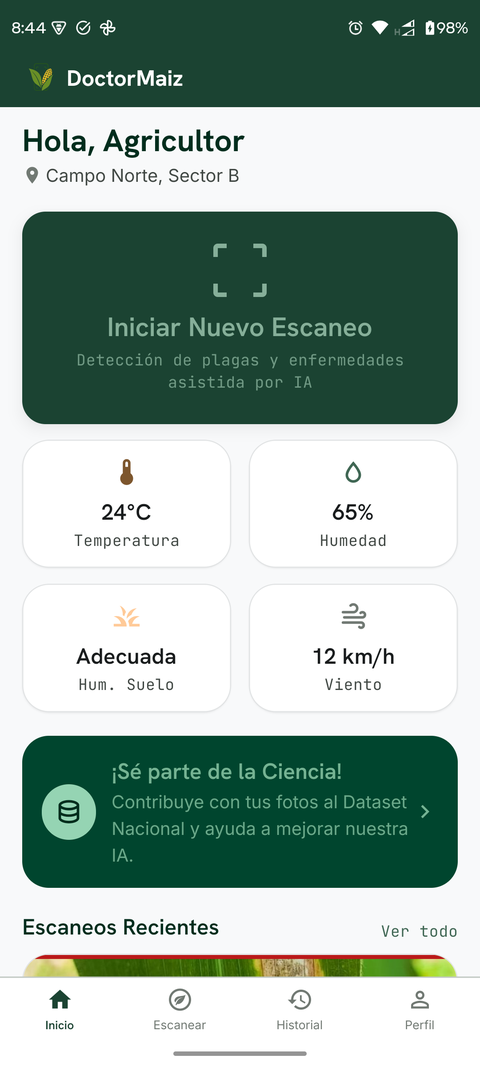
\includegraphics[width=\linewidth]{images/app/home.png}
\caption{Pantalla de inicio.}
\label{fig:app_home_c3}
\end{minipage}
\hfill
\begin{minipage}[b]{0.31\linewidth}
\centering
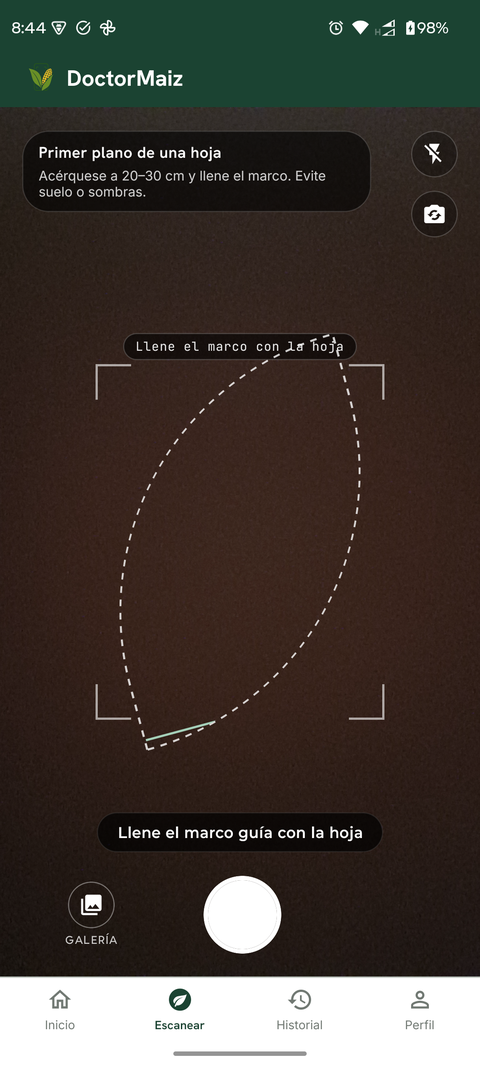
\includegraphics[width=\linewidth]{images/app/camara-marco-guia.png}
\caption{Marco gu\'ia foliar.}
\label{fig:app_cam_c3}
\end{minipage}
\hfill
\begin{minipage}[b]{0.31\linewidth}
\centering
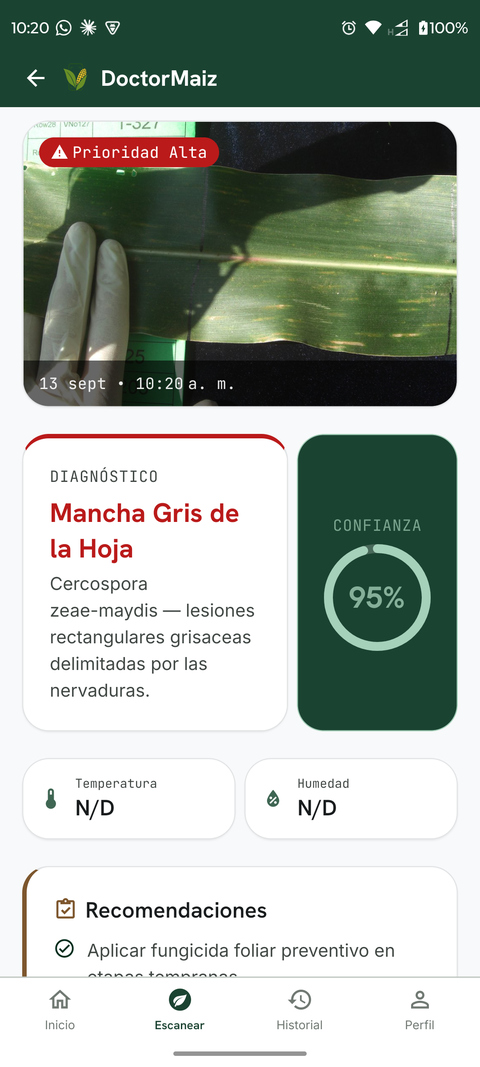
\includegraphics[width=\linewidth]{images/app/resultado-mancha-gris.png}
\caption{Diagn\'ostico obtenido.}
\label{fig:app_res_c3}
\end{minipage}
\caption{Flujo principal de la aplicaci\'on m\'ovil nativa DoctorMaiz.}
\label{fig:app_pantallas_1}
\end{figure}

\begin{figure}[H]
\centering
\begin{minipage}[b]{0.31\linewidth}
\centering
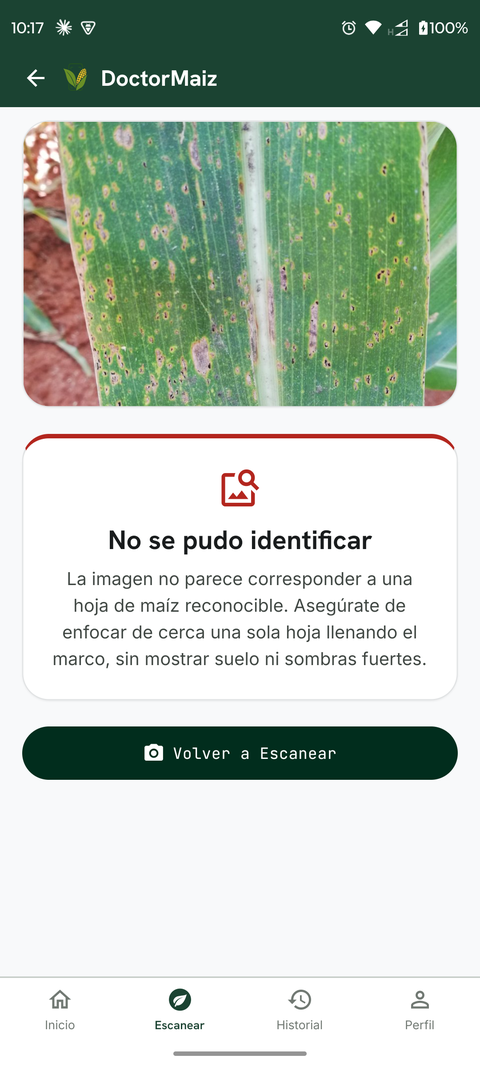
\includegraphics[width=\linewidth]{images/app/resultado-no-reconocida.png}
\caption{Bloqueo seguro por OOD.}
\label{fig:app_ood_c3}
\end{minipage}
\hfill
\begin{minipage}[b]{0.31\linewidth}
\centering
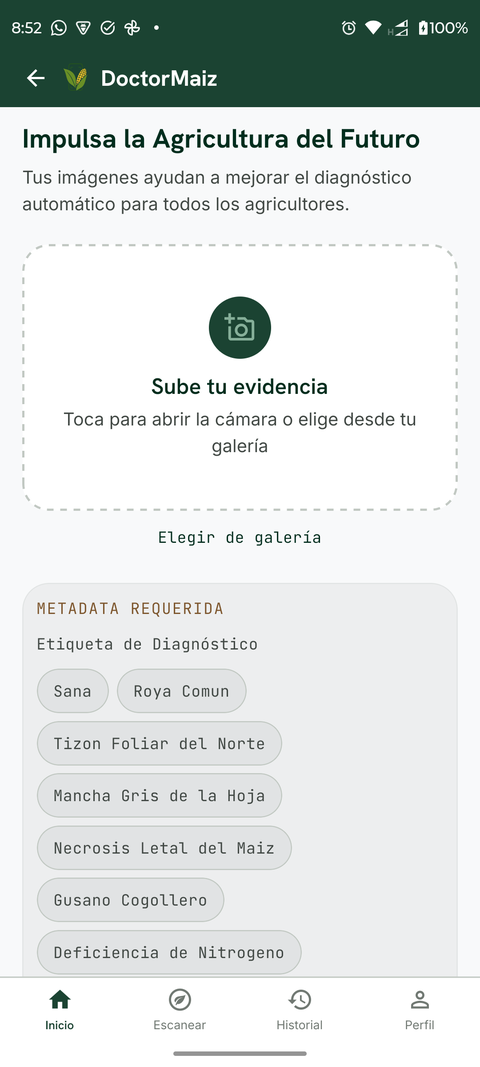
\includegraphics[width=\linewidth]{images/app/contribuir.png}
\caption{Aporte comunitario.}
\label{fig:app_contrib_c3}
\end{minipage}
\hfill
\begin{minipage}[b]{0.31\linewidth}
\centering
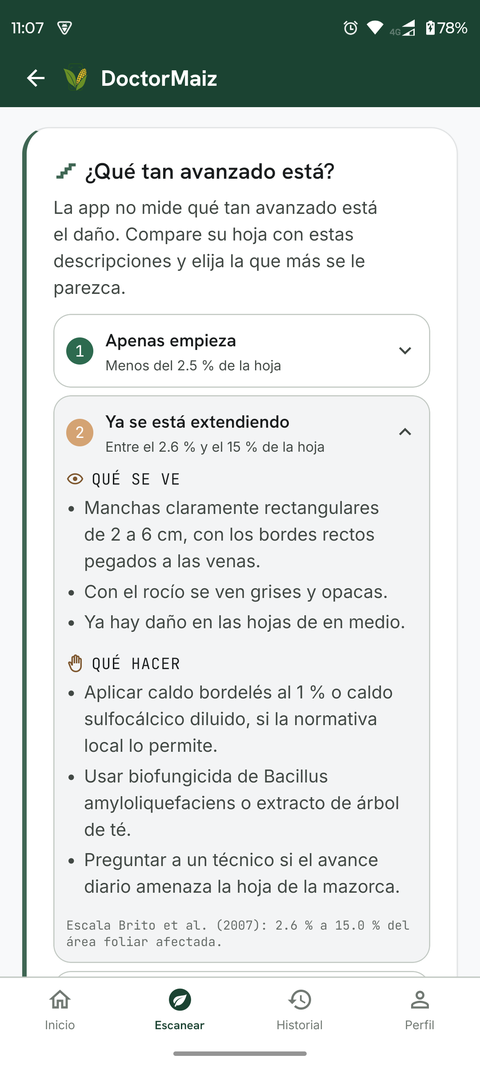
\includegraphics[width=\linewidth]{images/app/resultado-severidad.png}
\caption{Gu\'ia de severidad.}
\label{fig:app_sev_c3}
\end{minipage}
\caption{Mecanismos de seguridad, participaci\'on comunitaria y escalas agron\'omicas.}
\label{fig:app_pantallas_2}
\end{figure}

\section{Impacto Social y Recomendaciones de Pol\'itica P\'ublica}

El valor de esta investigaci\'on se consolida al traducir los avances matem\'aticos en cinco propuestas concretas dirigidas al Ministerio de Agricultura y Ganader\'ia (MAG) y al CENTA:

\begin{enumerate}
\item \textbf{Adopci\'on de DoctorMaiz como herramienta oficial de extensi\'on:} Homologar la app como asistente de bolsillo para los m\'as de 300 promotores del CENTA, estandarizando diagn\'osticos en caser\'ios remotos de Caba\~nas y Moraz\'an sin consumir datos celulares.
\item \textbf{Red Nacional de Alerta Fitosanitaria Temprana:} Alimentar un tablero epidemiol\'ogico centralizado en el MAG sincronizando an\'onimamente fechas y coordenadas de capturas cuando haya cobertura, activando cercos sanitarios ante rebrotes de necrosis letal.
\item \textbf{Banco Nacional Participativo de Datos Agr\'icolas:} Financiar brigadas fotogr\'aficas participativas junto a estudiantes de la Universidad de El Salvador para capturar variedades locales (h\'ibrido H-59 y criollos), cerrando definitivamente la brecha de dominio detectada.
\item \textbf{Campa\~nas comunitarias de alfabetizaci\'on digital agropecuaria:} Ense\~nar a cooperativas y ADESCOs el uso correcto del marco gu\'ia, posicionando la IA como aliada del saber campesino y no como sustituto.
\item \textbf{Soberan\'ia tecnol\'ogica y protecci\'on de datos campesinos:} Conservar el software bajo licencias de c\'odigo abierto (MIT/Apache 2.0), impidiendo la privatizaci\'on del patrimonio de datos agr\'icolas por transnacionales de semillas.
\end{enumerate}

\chapter*{Conclusiones y Recomendaciones}
\addcontentsline{toc}{chapter}{Conclusiones y Recomendaciones}

\section*{Conclusiones}

La presente investigaci\'on consolida la transici\'on desde una prueba de concepto preliminar hacia un sistema integral, cient\'ificamente riguroso y desplegado operativamente en dispositivos m\'oviles para el agro salvadore\~no. A partir de los resultados cuantitativos y cualitativos obtenidos, se concluye:

\begin{enumerate}
\item \textbf{Rendimiento del modelo en partici\'on estratificada:} El ensamble heterog\'eneo por votaci\'on suave entre EfficientNet-Lite0, EfficientNet-B0 y ShuffleNet-V2 alcanz\'o un Macro $F_1$ de \textbf{0.9567}, una exactitud de \textbf{98.29\%} y un Macro Recall de \textbf{95.06\%} sobre 5~015 im\'agenes de prueba. Estos resultados son de una sola semilla y de una partici\'on que mezcla fuentes; se presentan como resultado hist\'orico de la configuraci\'on desplegada, no como validaci\'on de generalizaci\'on.
\item \textbf{Recall de necrosis letal (MLN):} En la partici\'on estratificada, el ensamble clasific\'o correctamente los 963 casos de MLN del conjunto de prueba. Bajo validaci\'on con fuente no vista, el recall de MLN baja a un rango de 0.79 a 0.81, por lo que la ausencia de falsos negativos no se generaliza y debe seguir monitoreada en campo.
\item \textbf{Generalizaci\'on entre fuentes:} La validaci\'on agrupada por procedencia reduce el Macro $F_1$ de 0.9311 a \textbf{0.6026} sobre las clases evaluables en cada pliegue. La diferencia supera la variabilidad entre semillas, pero no permite atribuirla a un factor \'unico. El ahorro de horas de GPU frente a una b\'usqueda sin poda temprana no fue medido.
\item \textbf{Capacidades del diagn\'ostico:} El \textit{Disparate Impact Ratio} entre laboratorio y campo real es \textbf{0.9778}, por encima del umbral de 0.80. La ablaci\'on espacial mostr\'o que, al ocluir el centro de la hoja, el modelo conserva un \textbf{79.46\%} de exactitud, y al ocluir la periferia cae a \textbf{42.25\%}. Esto indica sensibilidad al contexto de la escena; el an\'alisis de equidad registra un nivel de riesgo m\'as alto que el de la prueba central, y se reporta as\'i para su revisi\'on.
\item \textbf{Soluci\'on integral en hardware rural:} La cuantizaci\'on a 8 bits produjo un archivo de \textbf{3.56~MB}. En un smartphone f\'isico Motorola edge 40 neo, la inferencia tom\'o aproximadamente \textbf{60~milisegundos} en una ejecuci\'on de referencia, y la aplicaci\'on opera sin conexi\'on para la clasificaci\'on. La exactitud de la versi\'on cuantizada sobre el conjunto de prueba completo no fue medida.
\item \textbf{Mitigaci\'on en la interfaz:} La aplicaci\'on incorpor\'o un marco gu\'ia para la captura y un detector OOD basado en distancia de Mahalanobis relativa, con umbral calibrado al percentil 95. Su efecto sobre el sesgo de procedencia no ha sido medido.
\end{enumerate}

\section*{Recomendaciones}

\begin{enumerate}
\item \textbf{Transici\'on a ensayos de validaci\'on en campo:} Desplegar un programa piloto de validaci\'on participativa con cooperativas agr\'icolas y ADESCOs en los departamentos de Caba\~nas, Moraz\'an y Ahuachap\'an para evaluar la adopci\'on del marco gu\'ia bajo luz solar intensa y condiciones reales de campo.
\item \textbf{Consolidaci\'on del Banco Soberano de Datos:} Integrar de forma prioritaria las primeras 1~000 fotograf\'ias capturadas en milpas salvadore\~nas a trav\'es del m\'odulo de contribuci\'on comunitaria, permitiendo un reentrenamiento focalizado para cerrar la brecha de dominio detectada en la evaluaci\'on fuera de fuente.
\item \textbf{Anotaci\'on patom\'etrica para modelos ordinales de severidad:} Establecer un convenio t\'ecnico con fitopat\'ologos del CENTA para calificar un subconjunto de im\'agenes con escalas homologadas de severidad (Cobb modificada, Vieira, Brito), sentando las bases para cabezas de regresi\'on ordinal que predigan el grado de da\~no adem\'as de la clase.
\item \textbf{Adopci\'on y custodia institucional en el Estado salvadore\~no:} Promover que el Ministerio de Agricultura y Ganader\'ia adopte formalmente el c\'odigo y pesos de DoctorMaiz bajo gobernanza de c\'odigo abierto, asegurando que el conocimiento generado pertenezca a la sociedad y no a intereses corporativos transnacionales.
\end{enumerate}

% ----------------------------------------------------------------------
% BIBLIOGRAFÍA
% ----------------------------------------------------------------------
\newpage
\begin{thebibliography}{99}
\addcontentsline{toc}{chapter}{Bibliograf\'ia}

\bibitem{ahmad2023a}
Ahmad, A., El Gamal, A., \& Saraswat, D. (2023). Toward generalization of deep learning-based plant disease identification under controlled and field conditions. \textit{IEEE Access}, 11, 9042--9057.

\bibitem{baya2024}
Baya, J., et al. (2024). A mobile-based system for maize leaf disease detection and classification using machine learning algorithms and deep learning: A case study of ZeaWatch. \textit{Smart Agricultural Technology}, 7, 100412.

\bibitem{bcr2023}
Banco Central de Reserva de El Salvador (BCR). (2023). \textit{Revista Econ\'omica: Aporte Agropecuario al Producto Interno Bruto 2022-2023}. San Salvador: BCR.

\bibitem{centa2022}
Centro Nacional de Tecnolog\'ia Agropecuaria y Forestal ``Enrique \'Alvarez C\'ordova'' (CENTA). (2022). \textit{Gu\'ia t\'ecnica del cultivo de ma\'iz en El Salvador}. San Salvador: CENTA / Gerencia de Investigaci\'on y Transferencia.

\bibitem{deng2009}
Deng, J., Dong, W., Socher, R., Li, L.-J., Li, K., \& Fei-Fei, L. (2009). ImageNet: A large-scale hierarchical image database. En \textit{Proceedings of the IEEE/CVF Conference on Computer Vision and Pattern Recognition (CVPR)} (pp. 248--255).

\bibitem{gulrajani2021}
Gulrajani, I., \& Lopez-Paz, D. (2021). In search of lost domain generalization. En \textit{International Conference on Learning Representations (ICLR)}.

\bibitem{howard2017}
Howard, A. G., et al. (2017). MobileNets: Efficient convolutional neural networks for mobile vision applications. \textit{arXiv preprint arXiv:1704.04861}.

\bibitem{hu2018}
Hu, J., Shen, L., \& Sun, G. (2018). Squeeze-and-excitation networks. En \textit{Proceedings of the IEEE/CVF Conference on Computer Vision and Pattern Recognition (CVPR)} (pp. 7132--7141).

\bibitem{jacob2018}
Jacob, B., Kligys, S., Chen, B., Zhu, M., Tang, M., Howard, A., Adam, H., \& Kalenichenko, D. (2018). Quantization and training of neural networks for efficient integer-arithmetic-only inference. En \textit{Proceedings of the IEEE/CVF Conference on Computer Vision and Pattern Recognition (CVPR)} (pp. 2704--2713).

\bibitem{lee2018}
Lee, K., Lee, K., Lee, H., \& Shin, J. (2018). A simple unified framework for detecting out-of-distribution samples and adversarial attacks. En \textit{Advances in Neural Information Processing Systems (NeurIPS)}, 31.

\bibitem{lundberg2017}
Lundberg, S. M., \& Lee, S.-I. (2017). A unified approach to interpreting model predictions. En \textit{Advances in Neural Information Processing Systems (NeurIPS)}, 30, 4765--4774.

\bibitem{ma2018}
Ma, N., Zhang, X., Zheng, H.-T., \& Sun, J. (2018). ShuffleNet V2: Practical guidelines for efficient CNN architecture design. En \textit{Proceedings of the European Conference on Computer Vision (ECCV)} (pp. 116--131).

\bibitem{mag2023}
Ministerio de Agricultura y Ganader\'ia (MAG). (2023). \textit{Anuario de Estad\'isticas Agropecuarias y Seguridad Alimentaria en El Salvador 2022-2023}. San Salvador: MAG / Direcci\'on General de Econom\'ia Agropecuaria.

\bibitem{molnar2022}
Molnar, C. (2022). \textit{Interpretable Machine Learning: A Guide for Making Black Box Models Explainable} (2nd ed.). Munich: Christoph Molnar.

\bibitem{optuna2019}
Akiba, T., Sano, S., Yanase, T., Ohta, T., \& Koyama, M. (2019). Optuna: A next-generation hyperparameter optimization framework. En \textit{ACM SIGKDD Conference on Knowledge Discovery and Data Mining (KDD)} (pp. 2623--2631).

\bibitem{mahalanobispp2025}
Ren, J., et al. (2025). Mahalanobis++: Improving OOD detection via feature normalization. \textit{arXiv preprint arXiv:2505.18032}.

\bibitem{ren2021}
Ren, J., Fort, S., Liu, J., Roy, A. G., Padhy, S., \& Lakshminarayanan, B. (2021). A simple fix to Mahalanobis distance for improving near-OOD detection. \textit{arXiv preprint arXiv:2106.09022}.

\bibitem{ribeiro2016}
Ribeiro, M. T., Singh, S., \& Guestrin, C. (2016). ``Why should I trust you?'': Explaining the predictions of any classifier. En \textit{ACM SIGKDD Conference on Knowledge Discovery and Data Mining (KDD)} (pp. 1135--1144).

\bibitem{selvaraju2017}
Selvaraju, R. R., Cogswell, M., Das, A., Vedantam, R., Parikh, D., \& Batra, D. (2017). Grad-CAM: Visual explanations from deep networks via gradient-based localization. En \textit{Proceedings of the IEEE International Conference on Computer Vision (ICCV)} (pp. 618--626).

\bibitem{tan2019}
Tan, M., \& Le, Q. V. (2019). EfficientNet: Rethinking model scaling for convolutional neural networks. En \textit{International Conference on Machine Learning (ICML)} (pp. 6105--6114).

\end{thebibliography}

% ----------------------------------------------------------------------
% GLOSARIO
% ----------------------------------------------------------------------
\newpage
\chapter*{Glosario de T\'erminos}
\addcontentsline{toc}{chapter}{Glosario de T\'erminos}

\begin{description}
\item[Clever Hans Effect:] Fen\'omeno en el cual un modelo de aprendizaje autom\'atico alcanza una aparente alta precisi\'on apoy\'andose en correlaciones espurias o atajos del entorno (fondos, sensores, marcas de agua) en lugar de las caracter\'isticas intr\'insecas de la clase.
\item[Cosine Annealing:] Esquema de planificaci\'on de tasa de aprendizaje que reduce gradualmente el paso de optimizaci\'on siguiendo la curva de un coseno hasta un m\'inimo establecido, facilitando que el optimizador escape de m\'inimos locales.
\item[Disparate Impact Ratio (DIR):] M\'etrica de equidad algor\'itmica que cuantifica el cociente entre la tasa favorable del grupo minoritario y la del grupo mayoritario. Un valor inferior a 0.80 denota sesgo o trato dispar regulatorio.
\item[Edge AI:] Paradigma de inteligencia artificial donde los modelos entrenados se ejecutan directamente en hardware local (dispositivos m\'oviles, microcontroladores) sin enviar datos a servidores en la nube.
\item[Macro $F_1$-Score:] Media aritm\'etica no ponderada del valor $F_1$ calculado independientemente para cada clase. Asigna el mismo peso relativo a clases minoritarias y mayoritarias, siendo la m\'etrica est\'andar ante conjuntos desbalanceados.
\item[MLOps (Machine Learning Operations):] Conjunto de pr\'acticas de ingenier\'ia de software destinadas a automatizar, versionar y garantizar la reproducibilidad y monitoreo de pipelines de aprendizaje autom\'atico en producci\'on.
\item[Necrosis Letal del Ma\'iz (MLN):] Complejo viral devastador provocado por la coinfecci\'on sin\'ergica del virus del moteado clor\'otico del ma\'iz (MCMV) y un potyvirus (como SCMV), capaz de destruir el 100\% de una plantaci\'on.
\item[Out-of-Distribution (OOD):] Condici\'on que presentan aquellas muestras alimentadas a un clasificador cuyas caracter\'isticas estad\'isticas provienen de una distribuci\'on ajena a la utilizada durante el entrenamiento (ej. fotografiar una piedra o una mano frente a un modelo de hojas).
\item[Post-Training Quantization (PTQ):] T\'ecnica de optimizaci\'on que convierte los pesos y activaciones de una red neuronal entrenada en coma flotante (FP32) a enteros de precisi\'on reducida (Int8), disminuyendo el tama\~no del modelo y la latencia en CPU.
\item[Soft Voting:] Mecanismo de ensamble multimodelo que promedia las probabilidades continuas asignadas por cada red individual mediante la funci\'on Softmax, seleccionando la clase con el m\'aximo consenso medio.
\end{description}

% ----------------------------------------------------------------------
% ANEXOS
% ----------------------------------------------------------------------
\newpage
\chapter*{Anexos}
\addcontentsline{toc}{chapter}{Anexos}

\section*{Anexo A: Registro de Enlaces y Repositorios Abiertos del Proyecto}

El c\'odigo fuente \'integro, los pesos exportados, los pipelines de entrenamiento y los artefactos de evaluaci\'on de \textbf{DoctorMaiz} se encuentran p\'ublicamente accesibles bajo licencias de c\'odigo abierto:

\begin{itemize}
\item \textbf{Clasificador Principal (Entrenamiento, HPO y Exportaci\'on):}\par
\url{https://github.com/daiv05/maize-doctor-classifier}
\item \textbf{Aplicaci\'on M\'ovil Nativa DoctorMaiz (React Native Offline):}\par
\url{https://github.com/Edenilson-Molina/maize-doctor-app}
\item \textbf{Segmentador Foliar YOLO (Detecci\'on y M\'ascaras de Instancia):}\par
\url{https://github.com/abner-rivas/maize-doctor-segmenter-leaf}
\item \textbf{API de Sincronizaci\'on y Extensi\'on Centralizada:}\par
\url{https://github.com/daiv05/maize-doctor-api}
\item \textbf{Sitio Web y Documentaci\'on T\'ecnica del Proyecto:}\par
\url{https://doctor-maiz.deras.dev/es}
\item \textbf{Dataset Consolidado de 33K Im\'agenes en Hugging Face:}\par
\url{https://huggingface.co/datasets/daiv05/corn-leaf-diseases-pests-and-deficiencies}
\item \textbf{Repositorio de Checkpoints y Modelos Exportados en Google Drive:}\par
\url{https://drive.google.com/drive/folders/1OeZdWggfp7nVkaYHW_oOuCma5xbwhns6?usp=drive_link}
\end{itemize}

\section*{Anexo B: Inventario Criptogr\'afico de Checkpoints Respaldados}

La Tabla~\ref{tab:anexo_checkpoints} detalla los hashes SHA-256 de los principales checkpoints f\'isicos que sustentan la reproducibilidad de la tesina.

\begin{table}[H]
\caption{Hashes SHA-256 de los pesos f\'isicos de los modelos respaldados}
\label{tab:anexo_checkpoints}
\centering
\small
\begin{singlespace}
\begin{tabularx}{\textwidth}{p{4.0cm}cp{7.5cm}}
\toprule
\textbf{Modelo / Protocolo} & \textbf{Tama\~no} & \textbf{Hash SHA-256 del Checkpoint (\texttt{best.pth})} \\
\midrule
EfficientNet-Lite0 Base (42, oficial) & 12.92 MB & \path{860180f33bf1749ffee9f3cccb9569a47afd9ca0fcef52713e18f99f82a57859} \\
EfficientNet-Lite0 Int8 (M\'ovil, \texttt{model\_int8.tflite}) & 3.56 MB & \path{0a77ad7937f73e24b795288c68741d14dd00226ffe546d5ddf5b99125fbef24d} \\
EfficientNet-B0 Referencia & 16.36 MB & Pendiente de verificaci\'on \\
ShuffleNet-V2-x1.0 Referencia & 5.2 MB & Pendiente de verificaci\'on \\
\bottomrule
\end{tabularx}
\end{singlespace}
\end{table}


\end{document}
